\documentclass[12pt]{report}
\usepackage{amsmath}
\usepackage{amsfonts}
\usepackage{amssymb}
\usepackage{textcomp}
\usepackage{graphicx}
\usepackage{float}
\usepackage{hyperref}
\usepackage[a4paper, margin = 1in]{geometry}

\usepackage[draft]{todonotes}


%Commands used in text, edit here and the document will populate with correct value.
\newcommand{\projectName}{CEPAD }
\newcommand{\payLoadMass}{3.352Kgs }

\makeatletter
\newcommand*\bigcdot{\mathpalette\bigcdot@{.5}}
\newcommand*\bigcdot@[2]{\mathbin{\vcenter{\hbox{\scalebox{#2}{$\m@th#1\bullet$}}}}}
\makeatother

%*******************************TITLE PAGE*******************************%

\title{Development of a Close Quarter Collision Protected Aerial Drone}
\author{Angus Steele} 

%*******************************START OF DOCUMENT*******************************%

\begin{document}

\maketitle

%*******************************BEGIN THE ABSTRACT*******************************%

\chapter*{Abstract}
\todo[inline]{Incomplete}
The need for robots is evident. High costs of maintenance. High costs of shut-downs for personnel Inspections

%*******************************DOCUMENT LISTS*******************************%

\tableofcontents
%\listoffigures giving issues
\listoftables

%*******************************SELF GENERATED GLOSSARY*******************************%

\chapter*{Glossary}
\begin{enumerate}
%\item Close-Quarter Explosion Protected Aerial Drone (CEPAD)
\item Micro Aerial Vehicles (MAV)
\item Unmanned Aerial System (UAS)
\item Unmanned Aerial Vehicle (UAV)
%\item IECEx (International Electrotechnical Commission for Explosive Atmospheres)
%\item ATEX (Atmosph\`{e}res Explosives)
\item Disk Loading (DL)
\item Power Loading (PL)
%\item South African Bureau of Standards (SABS)
%\item South African National Standards (SANS)
%\item International Organisation of Standards (ISO)
\item Degree of Freedom (DOF)

\item On Board Computer (OBC)
\item Ground Control Station (GCS)
\end{enumerate}

%*******************************CONSISTENCY RULES*******************************%
\newpage

\todo[inline]{RULES FOR CONSISTENCY:}
\todo[inline]{}
\todo[inline]{Figure always with a capital F}
\todo[inline]{Equation, use eqref (or put in brackets) and don't say equation unless it's the beginning of a sentence}
\todo[inline]{Image citation done inline as well as "Taken from (X) in caption"}
\todo[inline]{Equation citation done inline only}
\todo[inline]{Section always with a capital S}

\todo[inline]{}
%*******************************INCLUDE DIFFERENT CHAPTERS*******************************%

\chapter{Introduction}
This chapter sets to lay out as an introduction to the research. By discussing the end use case of the design, a few critical research questions can be raised. A problem statement will be drawn out by these questions. The chapter will then be concluded with a list of extracted requirements that the system needs to address and ultimately accomplish. \todo{Needs editing}

	\section{Project Background}
	Tracked and wheeled robots are beginning to reach their limitations, and society is in need of more complex and versatile vehicles. For a land robot to successfully navigate an extremely complex or cluttered environment, the designer must look at creating a legged robot. Legged designs introduce complexity into any system due to the intensive control theory required. There has been some great progress in legged designs, such as Big Dog created by Boston Dynamics \cite{BigDog}. Nevertheless, deploying currently available legged platforms could cost valuable time with lengthy navigation routines. An alternative approach would be to use an aerial platform that could do overhead surveillance. A drone could complete the required task by flying over the complexities in the operating environment. However, with conventional flight techniques and platforms, almost any sort of collision would cause a failure and the system would not be able to complete its mission. This limits this approach to only work in a situation where the drone would be able to fly over the obstacles. 
	
	Unfortunately, many of the desired use cases are not open aired and the platform will be required to fly below and even through obstacles to complete its task. A good example of this is in search and rescue missions. An aerial vehicle will be required to navigate through damaged or even collapsed buildings. The same platform could be used in a mining environment. Used to assist miners in assessing unexplored and potentially dangerous areas. 
	From the late 1800s South Africa has had a massive mining community, with coal, gold and diamond mining being used as a major source of income and job creation for the country. In response to this, two South African research institutes have agreed to a joint collaboration in solving some of these aspects for an underground mine environment. This project involves both The University of Stellenbosch (US) and the Council of Scientific and Industrial research (CSIR). A mining environment has many applications for a collision resistant drone. Such as the mapping of unknown and potentially hazardous environments. The drone would be able to fly in, conduct a survey of the environment and feed that information back to the miners, ensuring a safer work environment while minimising costly delays. However, an underground mine introduces more variables than just potential collisions.
	
	\section{Problem Statement}
	There are many potential applications for a drone capable of close quarter flight. After discussions with the CSIR, \projectName was seen as a potential safety platform for use in mines. Unsafe underground territories create a need for unmanned vehicles to do inspections. These areas are currently been mapped by trained professionals who risk their lives going into these unsecured regions. Using land vehicles proves difficult and slow in the complex terrains, creating a need for an alternative solution.
	
	Designing any aerial drone introduces many complexities by itself, including obtaining the required aerodynamics to achieve stable flight. There are modules that one can buy to stabilise the craft, but in a confined indoor space, this specification gets enhanced with the need to stabilise itself after a collision or due to flight near surfaces as shown in \cite{}. 
	Several strategies will need to be investigated to assist the device in navigating these confined environments. The platform should attempt to maintain a set distance from the walls, floors and other obstructions.
	Instead of implementing complex and unreliable collision avoidance systems this platform will be designed for impact resistance. This project will also make the assumption that the robot will fly into obstacles during operations. This requirement affects the mechanical construction of the vehicle, but as stated above, intensifies the control laws required.
	For an indoor application it is important that the device can fly in a GPS constrained environment. Although this factor will not be solved in the scope of this project, the design of \projectName should consider some of the factors involved to ensure expansion into that research can be done with relatively small changes to the work accomplished here.
	
	To ensure the platform can be extended to industrial applications, certain external factors and peripherals need to be included. The device will need to be able to complete some of this missions autonomously, especially when line of sight and potentially communications are lost.
	The platform must be able to handle and interface to an array of sensors for each specific mission. The drone will need to be small to increase its accessibility in confined spaces, this will limit payload and flight time. To complete a useful mission the platform must be able to run for at least 20 minutes \todo{Check this time and if stating it is appropriate} or more.
	
	\section{Application Requirements}
	The problem statement above briefly introduces certain needs \projectName must solve, the section that follows attempts to address each of these points and define them more specifically as key requirements for the system as a whole. To begin, this statement of requirements can be started by creating two high level objectives, achieving flight in a confined indoor space and providing the ability to complete industrial applications. 
	
		\subsection{Controlled Indoor Flight}
		The identified requirements of the system begin by providing an aerial platform with the ability to fly in an enclosed, confined space. To do this, the platform must be able to position itself from any obstructions above, below or beside itself. This will require that the platform can measure its proximity to the surroundings in all directions. The flight controller must therefore be able to include additional sensor inputs into it's control laws and other real time processes. When a new obstruction is detected it must have the ability to steadily move away and reposition itself, while not straying too far off the mission plan.
		
		In order for the platform to complete missions in this environment, the drone needs to withstand the disturbances introduced by flight close to obstructions as well as collisions with these obstructions. This creates a requirement to mechanically protect the platform from irreversible damage caused by a collision. The flight controllers on board must be able to stabilise the platform post collision. Additional requirements are introduced due to disturbances by being in close proximity and not necessarily colliding with, walls, floors and other obstructions. The flight control must be equipped to handle the near wall/ground effect.
		
		\subsection{Method of Expansion for Industrial Applications}
		If the above requirements are met, the platform could be expanded into an array of industrial and research applications. Most of these use cases will require additional modes, sensors and other peripherals. Although not all these factors will be proven for in this project, they must be considered so that expansion into these realms can be done with minimal rework being needed on the platform.
		
		Since most of these missions will require some level of autonomy, the chosen flight controls must include an autopilot flight mode that allows the user to switch between manual and automatic mode. There must be a method to send flight data back to a ground control station for real time analysis of the mission. The ground control station should be able to update or halt the mission plan during deployment. Since additional sensors will be required, the platform must include some interface to handle the sensor data and relay the live sensor data back to a ground control station. The platform must provide a mechanism of mounting an array of different sensing equipment on board. This includes accounting for the extra thrust and electrical power requirements added by the sensors. Finally the drone must be able to stay in the air long enough to complete a mission. With indeterminable mission lengths at this point, the device must be able to expand it's battery capacity to account for longer missions.
	
	\section{Assumption and Limitations}
		\subsection{Location Sensing}
		\subsection{Route Planning Strategy}
		\subsection{Modelling Errors}
		In order to limit the effect of modelling errors, this project has followed a stringent system identification process. However no model is error free  

\chapter{Literature Review}
This chapter seeks to evaluate existing research in the field of rotorcraft design and obstacle avoidance strategies. To critically review some of the high level concepts in rotorcraft design, a brief evaluation is given of flight theory and how they effect design decisions for rotorcraft. After an understanding of flight theory is obtained, it is necessary to evaluate how this theory is utilised in creating rotorcraft. Armed with a better understanding of flight generation for rotorcraft, an analysis of traditional rotorcraft configurations is completed. Due to the hazardous nature of the mission environments, existing collision protection techniques are then discussed. At this point, the reader should feel confidence that the platform design is grounded with a solid understanding of existing techniques and requirements.
Now that a platform has been developed, the next step is to review some of the methods used to control multi-rotor platforms. Once stable flight methods have been evaluated and discussed, the researcher reviewed existing methods for obstacle avoidance as well as the requirements of implementing an on-board obstacle avoidance system.

\section{Flight Theory}

Although there are many different forms of flight, each form will have a very similar force diagram as seen in Figure \ref{IM_FlightForces}. 

\begin{figure}
\centering
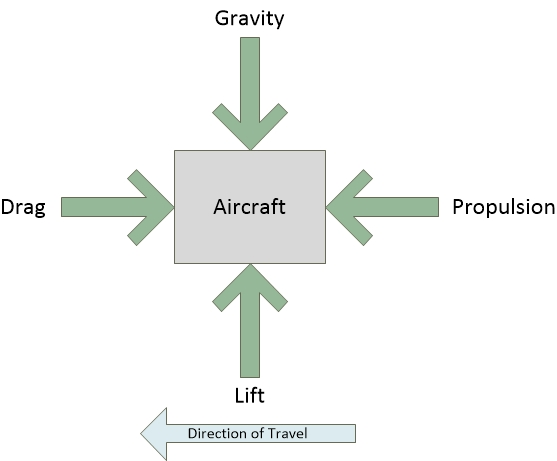
\includegraphics[height = 6cm]{Images/Literature/Flight}
\caption{Force diagram of basic components of flight}
\label{IM_FlightForces}
\end{figure}

From the force diagram it can be intuitively seen that to increase the velocity of a body in air, the lift must exceed the weight.
Weight is directly determined by the object's mass and the relevant gravity coefficient, $W = mg$. Lift counteracts this weight in an attempt to boost the body into the air. Upward acceleration is only achieved once lift exceeds weight, if they are equal the body will be in a state of hover. From the lift equation seen in \eqref{EQ_Lift} only a body with velocity can obtain lift. In a rotorcraft, the rotating blades move through the air and generate lift, thereby negating the requirement for the body to have any linear velocity. Unlike in a fixed wing aircraft if the vehicle is stationery, zero lift is generated, thus a vertical take-off is not possible. 

\begin{equation}
\label{EQ_Lift}
Lift = C_L(\frac{1}{2} \rho V^2) S
\end{equation}

To propel the body forward the propulsion must exceed the value of the drag force, which acts directly against its velocity vector. When no propulsion force is present, the craft will continue to lose speed due to drag. Similar to lift, drag varies with velocity as shown in equation (\ref{EQ_Drag}).

\begin{equation}
\label{EQ_Drag}
Drag = C_D (\frac{1}{2} \rho V^2) A
\end{equation}

The coefficient of drag ($C_D$) is determined by the objects shape and ultimately the way it interacts with the air flow. 

Figure \ref{IM_FlightForces} better describes a fixed wing aircraft, the lift and propulsion forces in a rotorcraft can be seen as the components of thrust which generate either a vertical or horizontal force. To better understand the design behind rotorcraft, the principles behind this thrust generation are discussed.

	\subsection{Fundamental Principles of Flow}
	Rotors generate thrust by pulling quiescent air through the rotor plane. The principles that best govern these flow dynamics and force generation are discussed below.
	
		\subsubsection{Continuity Equation and Bernoulli's Principle}
		Bernoulli observed that the mass flow in a closed system remains constant, as shown in \eqref{EQ_BernoulliP}. This principle states that in a closed system, the product of density ($\rho$), area (A) and velocity (v) for a flowing system will remain constant \cite{Dayle}. Based on this finding it was discovered that the mass flow of a flowing medium will follow the laws of continuity in the form of equation \eqref{EQ_Bernoulli}.
		
		\begin{equation}
		\label{EQ_BernoulliP}
		\Delta \rho Av = 0
		\end{equation} 
		
		The Bernoulli equation is a statement of the conservation of energies present in a flowing system \cite{Dayle}. Equation \ref{EQ_Bernoulli} considers a pipe with a flowing liquid and states that the energy will remain unchanged in a closed system. The sum of these energies will contain the kinetic energy of the liquid as well as the energy present through pressure. Bernoulli's equation can be rewritten in the form \eqref{EQ_Bernoulli2} to represent that any changes in pressure, can result in a change of the velocities.
		
		\begin{eqnarray}
		P_0 + \frac{1}{2} \rho v_0^2 &=& P_1 + \frac{1}{2} \rho v_i^2\label{EQ_Bernoulli}\\
		P_2 - P_1 &=& \frac{1}{2} \rho (v_\infty^2 - v_0^2)\label{EQ_Bernoulli2}
		\end{eqnarray}

		\subsubsection{Reynold's Number}
		Moving different objects in the same environment will create different results of flow, in the same breath moving the same object through different environments will also create various results of flow. Osborne Reynold attempted to mathematically determine these effects and quantify what caused a system to have turbulent flow opposed to laminar flow and vice versa. During his research he created a dimensionless constant known as the Reynold's number, as shown in equation \ref{EQ_Reynold} \cite{Reynold}. 
		
		\begin{equation}
		\label{EQ_Reynold}
		Re = \frac{\rho v L}{\mu}
		\end{equation} 
		
		In its simplest form, the Reynold's number of an object is the ratio between inertial forces ($\rho v L$) and viscous forces ($\mu$) of the gas. In a system where the viscous forces dominate ($Re ~< 10^3$), there will be laminar flow and when there are higher inertial forces ($Re >~ 10^4$) the flow will be turbulent. 
		Since turbulent flow will decrease stability and increase drag forces, Reynold's numbers have become a very important part in correctly modelling and designing aircraft \cite{Reynold}.

	\subsection{Basic Rotor Theory}
	The rotor is responsible for all the aspects of flight and generates the lift, forward propulsion and the means to control the orientation of the craft \cite{Leishman}. It is for this reason that an in depth understanding of rotor characteristics and performance was done. The original research into rotor analysis was done with helicopters, but the rotor theory basics are relevant to any rotating winged craft.
	
	Due to Newton's third law, any rotating blade will cause a a rotation in the opposite direction to that motion. This applied force will drive the vehicle to rotate around that spinning axis and creates the need for a counter torque mechanism. This is common with most rotorcraft and can be visualised in figure \ref{IM_Antitorque}, in the form of the tail rotor as seen in conventional helicopters. The quadrotor handles this by having an equal number of oppositely rotating rotors.
	
	\begin{figure}[H]
	\centering
	\includegraphics[height = 6cm]{Images/Literature/AntiTorque}
	\caption{Image Illustrating generation of Counter Torque (Taken from \cite{Heli})}
	\label{IM_Antitorque}
	\end{figure}
	
	The capability of any part of a rotor to produce lift is influenced by the local blade position and pressure at that point \cite{Leishman}.

	Angular velocity equations state that the speed of any part of the rotor varies along the length of the rotor. With the maximum velocity sitting at the rotor tip. As the rotor spins, the blade's angle of attack shifts. This angle is defined as an azimuth angle ($\psi$) and is measured relative to air flow. The azimuth angle is 0\textdegree down stream and sits at 180\textdegree when it faces directly upstream. As the rotorcraft adds a horizontal component to its hover or vertical flight, the relative speed of the individual rotor segments now adheres to equation \eqref{EQ_TipSpeed}.  As visualised in figure \ref{IM_TipSpeed}, the relative velocity at the any part of the rotor is affected by the azimuth angle of the blade ($\psi$), translational speed of the craft ($V_{\infty}$), angular speed of the rotor ($\Omega$) and the considered distance along the rotor blade (r) \cite{Leishman} \cite{RotorCraftHand}. 

	\begin{figure}[H]
		\centering
		\includegraphics[height = 6cm]{Images/Literature/TipSpeed}
		\caption{Velocity components of a rotor \cite{Leishman}}
		\label{IM_TipSpeed}
	\end{figure}
		
	\begin{equation}
	\label{EQ_TipSpeed}
	V_{r} = \Omega r + V_{\infty}\sin(\psi)
	\end{equation}
	
	What this relationship shows is that during forward flight the tip velocity, relative to the ground, changes even if the rotor rotates at a constant speed. This complicates the rotor dynamics at higher speeds and limits the top speed of the craft. On the retreating edge ($\psi = 270$\textdegree $\therefore sin(\psi) = -1$) if $\Omega r <= V_{\infty}$ the rotor would effectively be going backwards and the helicopter is at risk of stalling out, this is known as a stall condition \cite{Leishman} \cite{RotorCraftHand}, while the advancing edge is reaching its maximum speed by approaching Mach conditions and sever instability.

	\subsection{Momentum Theory and Thrust Basics}
	
	As mentioned above the rotors of a rotorcraft are responsible for generating all the forces that manoeuvre the vehicle. These forces are induced by pushing air through the rotor disk. With a fixed wing aircraft the analysis of the blades is simplified because the only air flow produced is from the translational velocity of the entire craft. Analysis of blade performance in a rotorcraft can be more challenging as the rotation of the blades must be considered along side the overall speed of the vehicle. As the craft manoeuvres in space, the air flow through the rotor has significant complexities which complicates the analysis. Since the rotorcraft is expected to perform in a variety of flight styles it is important to understand these models, and their flaws. 
	
	To simplify, initially consider a helicopter in a hovering state (Weight(W) = Thrust(T)). Figure \ref{IM_MomentumTheoryAirFlow}, taken from \cite{Leishman}, helps visualise the induced air flow by showing how the rotor smooths out the air by forcing it through the disk area. This more uniform air creates an edge known as the slipstream or wake boundary, with the surrounding air remaining dormant \cite{Leishman}. Inside the wake boundary, the average velocity of the air is tangible and effective, where outside the slipstream edge, the average air velocity is negligible and obsolete. The force required to push that mass of air through the disk space is, by Newton's third law, returned by the air unto the rotor. Thus giving the rotor blades a thrust component.
	  
	\begin{figure}[h]
	\centering
	\includegraphics[height = 8cm]{Images/Literature/MomentumTheoryAirFlow}	
	\caption{Visualisation of Induced Air Flow Through A Rotor \cite{Leishman}}
	\label{IM_MomentumTheoryAirFlow}
	\end{figure}
	
	Rankine-Froude's Momentum Theory looks at this induced velocity as well as the displacement of air through the propeller, and attempts to quantify the induced thrust. While figure \ref{IM_MomentumTheoryAirFlow} helps visualise the principle, the variable naming convention for the equations is shown in figure \ref{IM_MomentumTheoryHover} below. 
	Labels 0, 1, 2 and $\infty$ refer to the locations of quiescent flow, inflow directly before the rotor, airflow immediately after the disk and the slipstream\footnote{Generally far wake is considered as 1 full rotor diameter distance away \cite{Leishman}.} or far wake condition respectively.
	The velocities are shown as the induced velocity in and out the rotor ($v_{i}$), the far wake velocity ($v_{\infty}$) and finally $v_{0}$ represents the zone with zero flow rate. There is no velocity jump across the rotor, the energy being fed into the system by the rotor is represented by a pressure change.
	
	\begin{figure}[h]
	\centering
	\includegraphics[height = 8cm, angle=360]{Images/Literature/MomentumTheoryHover}			%Must show both air flow as well as far stream and such
	\caption{Momentum Theory in Hover (Adapted From \cite{Leishman})}
	\label{IM_MomentumTheoryHover}
	\end{figure}
	
	As described above, it is by forcing the air through the disk that lift is generated. The mass flow rate of this air can then be described by (\ref{EQ_MassFlow}), where ($\rho$) is the density of air and A is the area of one full blade rotation. The rate at which this mass of air is displaced becomes a crucial variable in rotor dynamics and is directly proportional to thrust (T). This relationship can be quantified as shown in (\ref{EQ_ThrustBasic}). Thrust can also be calculated by finding the difference in pressures over the rotor disk as in (\ref{EQ_ThrustPressure}). Since acceleration is the difference in $v_\infty$ and $v_0$, \eqref{EQ_ThrustMass} can also be obtained.
	
	\begin{eqnarray}
	\dot{m} &=& \rho A v_{i}\label{EQ_MassFlow}\\
	T &=& \dot{m}a\label{EQ_ThrustBasic}\\
	T &=& A(P_2 - P_1)\label{EQ_ThrustPressure}\\
	T &=& \rho A v_{i} (v_\infty - v_0)\label{EQ_ThrustMass}
	\end{eqnarray}
	
	Equation \eqref{EQ_ThrustMass} demonstrates the negative effect of having active ambient air. This could be caused by surrounding turbulent airflow, wind or even translational movements and will need to be considered in the controller design.

	\subsection{Disk and Power Loading}
		\subsubsection{Disk Loading}
		Disk loading (DL) is a term seen often in the world of rotorcraft, it is a simple but important ratio between thrust and the area a rotating disk makes. It is represented in \eqref{EQ_DL}. Since the pressure drop across each rotor is considered uniform, the disk loading for each rotor will equate to the pressure drop across that disk.
		 
		\begin{equation}
		\label{EQ_DL}
		DL (\frac{N}{m^{2}})= \frac{T}{A} = \frac{1}{2} \rho v_\infty^2
		\end{equation}
		
		For multi-rotor craft, the disk loading is assumed uniform across all rotors \cite{Leishman}. The overall disk loading of a single rotorcraft such as a traditional helicopter will be lower than that of a multi-rotor craft of a similar size \cite{RotorCraftHand}.  Figure \ref{IM_DL} shows some examples of disk loading values for a variety of rotor configurations, as shown disk loading is also a measure of hover efficiency.
		\todo{Edit this graph to include multirotors}
		\begin{figure}[H]
		\centering
		\includegraphics[height = 6cm]{Images/Literature/DL}     
		\caption{Image representing, various Disk Loading values for varying rotorcraft (Taken from \cite{Leishman})}
		\label{IM_DL}
		\end{figure}
		
		A higher disk loading value results in larger values for induced velocities as well as the required power to hover. This means that the larger the blades, the better the efficiency. More force will be generated by pushing large quantities of air slowly, than forcing small amounts of air through at high speeds. Of course with bigger blades, comes larger rotational inertia and geometry as well as the craft being less immune to gusts and interferences. A larger blade also creates faster tip velocities, which will limit the speed of the craft severely \cite{Leishman}.
		
		
		
		\subsubsection{Power Loading}
		Power is given by the product of both Thrust and the induced velocity at the blade. It can be written as shown in equation (\ref{EQ_Power}). What this ratio shows is that the ideal power is in cubic proportion to the induced velocity at the rotor. Therefore to reduce required power the rotor's induced velocity must be small, which can be accomplished by a significant increase in disk area \cite{Leishman}.
		
		\begin{equation}
		\label{EQ_Power}
		P = 2 \rho A v_{i}^3
		\end{equation}
		
		Another important ratio is between thrust and power, it is called power loading (PL) and is shown in equation (\ref{EQ_PL}). Power loading can be seen as a measure of craft efficiency. 
		
		\begin{equation}
		\label{EQ_PL}
		PL (\frac{N}{kW})= \frac{T}{P}
		\end{equation}
		
		From equations \eqref{EQ_DL} and \eqref{EQ_PL} it can be shown that power loading is inversely proportional to disk loading. Therefore a craft with a lower disk loading will generally be a more efficient platform.

	\subsection{Electrical Power to Thrust}
	Equation (\ref{EQ_Power}) gives a quantitative approach to solving for aerodynamic power ($P_i$). If electrical power is taken as $P_e = VI$, where V is the applied voltage and I is the sourced current, with an efficiency of $\eta$ then $P_i = \eta VI$. Noting that $P_i = T v_i$ and using equation (\ref{EQ_Power}), a relationship between thrust and $P_e$ can be formed and is represented in equation (\ref{EQ_ElectricalPowerThrust}).
	
	\begin{equation}
	\label{EQ_ElectricalPowerThrust}
	T = (2\rho A)^{\dfrac{1}{3}} (\eta P_e)^{\dfrac{2}{3}}
	\end{equation}
	
	Equation (\ref{EQ_ElectricalPowerThrust}) brings to light a very important relationship which states that thrust grows at a slower rate than the electrical input power to the system.
	
	\begin{equation*}
	T \propto P_e^{\dfrac{2}{3}}
	\end{equation*}

\section{Analysis of Conventional Rotor Wing Configurations}

Some of the fundamental theories described above relate to the basics behind various rotor configurations and even varying flight techniques. Each different arrangement of blades introduces certain advantages and disadvantages to the system. Not every configuration will be applicable for all operations and it is important to determine what criteria are critical for the intended application.  An analysis of varying rotor configurations is done below and follows a similar trend to that seen in \cite{RotorConfig}, \cite{Bohorquez} and \cite{NewMAV}. The main weighted criterion for the discussion were listed in no particular order as:

\begin{enumerate}
	\item Flight time and efficiency
	\item Geometry and size
	\item Drone Manoeuvrability
	\item Control algorithms
	\item Mechanical complexity
\end{enumerate}

Before the analysis can be done, certain operating parameters of the different craft, surrounding the above mentioned criteria, need to be understood. There has been discussions regarding why and how rotor blades produce lift, this section discusses the real world implementation of those blades.


The same way that a car tyre is the only way the energy from the engine is translated into motion, the rotor in a rotorcraft is responsible for taking the kinetic energy from the motors and translating it into flight. Typically a rotorcraft will be designed with either fixed pitched, or variable pitched rotors. A fixed pitched rotor is a rotor that has an optimally selected, unchangeable pitch and therefore a fixed angle of attack. This of course means that since the angle of attack is fixed for the blade, an increase in speed will be required for a change in lift. With a variable pitched blade, the pilot can change the angle of attack to increase the forces. As the angle of attack increases, the blade will produce more lift without changing the speed of the motor. However, as the pitch increases, so does the drag of the blade. This then requires more motor power to keep the blade moving through the air.
The power requirements for either system are fairly similar, the advantages of a varying pitch is a single rotor has the potential for more dynamic force applications. The downfall however is the high level of complexity in the mechanical design. Both of these factors become pertinent in the final decision making of the platform design.

It is also known that any rotating member will produce a counter rotating torque to the static body, which means that any system with only one rotor will have inherent instability in the yaw axis. The end goal is to have a craft that can fly stably and accurately in 3 dimensions.

Having only a single, fixed pitched rotor allows only for control in the amount the craft flies up or down, as well as this fore mentioned instability. There are many different methods to obtain full six degrees of flight freedom. The following discussion tries to address each point listed above for different traditional methods, while trying to achieve an optimised design.


\subsection{Helicopter}
A conventional helicopter is still the most widely used configuration for large rotorcraft \cite{RotorConfig}. It consists of a single main rotor, coupled with a smaller counter rotating rotor located in the tail as seen in figure \ref{IM_Helicopter}\footnote{(Adapted from \cite{Heli})}, this is to counteract the developed counter torque as shown in Figure \ref{IM_Antitorque}.

\begin{figure}[H]
	\centering
	\includegraphics[height = 6cm]{Images/Literature/MainHeliComponents}     
	\caption{Main Components of a helicopter (Taken from \cite{Heli})}
	\label{IM_Helicopter}
\end{figure}

The main rotor of a standard helicopter has very low disk loading which gives it excellent hover efficiency. Since the desired end product will mostly be in a state of hover or at least slow lateral movement, this will yield good results for flight time. To achieve yaw stability this configuration makes use of a small tail rotor to counter act the induced moments. The extended tail rotor requires energy which it will draw from the motor while also adding a significant amount of length and weight to the craft. Since the single rotor only gives the pilot thrust control and the tail rotor gives measurable yaw control, there is need for more control surfaces to do more manoeuvring. To implement this most helicopters use a variable pitched rotor system. Cyclic control of this pitch allows the pilot to adjust the angle of attack of the rotor blades while they rotate, thus a forward pitch can be applied by increasing the lift on the left\footnote{This is true for an American style helicopter. The French design requires am increase of lift to the right}. This set up is mechanically very complex and takes intensive control algorithms and laws to give stable control.

Even though the classic helicopter image is always seen as a main rotor with a smaller rotor at the tail, there are many different types of anti torque tail set ups. The ducted fan approach increases the efficiency of the tail rotor by channelling the air flow of the rotor. The NOTAR design \cite{US4200252} as seen in Figure \ref{IM_NOTAR} manipulates the airflow generated by the main rotor and directs it to counter act the induced torque. A tip-jet design eliminates the torque applied to the airframe and therefore no tail rotor is required \cite{RotorConfig}. 

\begin{figure}[H]
	\centering
	\includegraphics[height = 6cm]{Images/Literature/NOTAR}     
	\caption{Image demonstrating the NOTAR system (Taken from\cite{Heli})}
	\label{IM_NOTAR}
\end{figure}

There have been many attempts at improving the standard helicopter design. These improvements have taken the form of adding rotors, designing hybrid aircraft and complex mechanical designs to harvest advantages of both the fixed wing and VTOL craft. Some have even tried to combine multiple features as Flanigan \cite{US7147182} did in his design of a tip-jet, compound, tilt rotor aircraft. 
In an attempt to keep the mechanical complexity to a minimum, not all configurations were investigated.

\subsection{Coaxial Rotors}
A coaxial configuration consists of two counter rotating blades located about the same centre of rotation that both use the same drive system. This eliminates the need for a tail rotor as the torque applied by both rotors cancel each other out, as shown in figure \ref{IM_Coaxial}.  

\begin{figure}[H]
	\centering
	\includegraphics[height = 6cm]{Images/Literature/Coaxial}     
	\caption{A standard Coaxial rotor set up and the induced forces}
	\label{IM_Coaxial}
\end{figure}

Localising the blades around a single point helps with the geometry of the craft as it is a more compact design. Using fixed pitched rotors, this platform will only give yaw and over all thrust control. Bohorquez et al in \cite{Bohorquez} attempted a number of lateral control methods, eventually settling on aerodynamic flaps to control the flow of the downwash, that and other methods are shown in figure \ref{IM_Coaxial_Variations}. Briod et all also used the same set up in his team's design of the Gimball \cite{Briod2012}.

\begin{figure}[H]
	\centering
	\includegraphics[height = 3cm]{Images/Literature/Coaxial_Configs}     
	\caption{Different methods of lateral control in a Coaxial MAV (Adapted from \cite{Bohorquez})}
	\label{IM_Coaxial_Variations}
\end{figure}

The control flaps are the most common used form of lateral control for small coaxial MAVs. They introduce little mechanical complexity and do not require excessive power to use. The flaps do however decrease efficiency of the system by interfering with the rotor airflow. If designed correctly the flaps should only influence the system while in use. For hover and vertical flight the impact will be negligible. As a control surface the flap is quite rudimentary and will require some more advanced control methods as well as in depth testing to obtain smooth flight transitions. Due to its compactness the design can have considerable manoeuvrability if the control algorithms are designed effectively. Each flap will require an actuator, this will increase total weight, power consumption and required mechanics \cite{Bohorquez}. 

The overlap of the rotors also induces an inefficiency into the system. Johnson in \cite{HeliTheory}, says there is much debate in how the loss of power is calculated. He states two of his preferred methods, the method chosen has a better approximation for small overlaps and is shown in \eqref{EQ_OverlapEfficiency} \cite{HeliTheory}. $\Delta P$ is the interference power (considered here as a fraction of total power) and $m$ is the overlap fraction and is calculated in \eqref{EQ_Overlap} \cite{HeliTheory}.

\begin{equation}
\label{EQ_OverlapEfficiency}
\frac{\Delta P}{P} = (\frac{2}{2-m})^{1/2} - 1
\end{equation}

\begin{equation}
\label{EQ_Overlap}
m = \frac{2}{\pi} \Bigg[ \cos^{-1}\frac{l}{2R} - \dfrac{l}{2R}\sqrt{1 - {\dfrac{l}{2R}}^2} \Bigg]
\end{equation}

These quantities assume a small vertical separation so that the inflow rates of both rotors can be considered the same. To calculate the overlap function, the rotor radius $R$ is needed as well as the separation distance $l$. 

\subsection{Tandem Rotors}

A tandem rotorcraft is sometimes referred to as a dual rotor, as it consists of two blades to generate thrust and thereby decreasing disk loading and increase the lift capacity. In a tandem configuration the blades sit in the front and the rear of the craft. Tandems are often used in applications that require heavier loads than the traditional rotorcraft can effectively offer. A tandem configuration is demonstrated in Figure \ref{IM_Tandem}\footnote{Image taken from https://www.snafu-solomon.com/2011/11/ch-46-flight-ops-aboard-uss-new-orleans.html}, the blades spin in opposite directions to counteract the other's rotational torque. Pitch and Yaw control are readily available through manipulation of the rotor speeds, while roll control is not as easily accomplished with this design and generally require variable pitch rotors \cite{Oh2005}. Using two smaller blades also decreases the effects of interferences such as gusts on the craft. 

\begin{figure}[H]
	\centering
	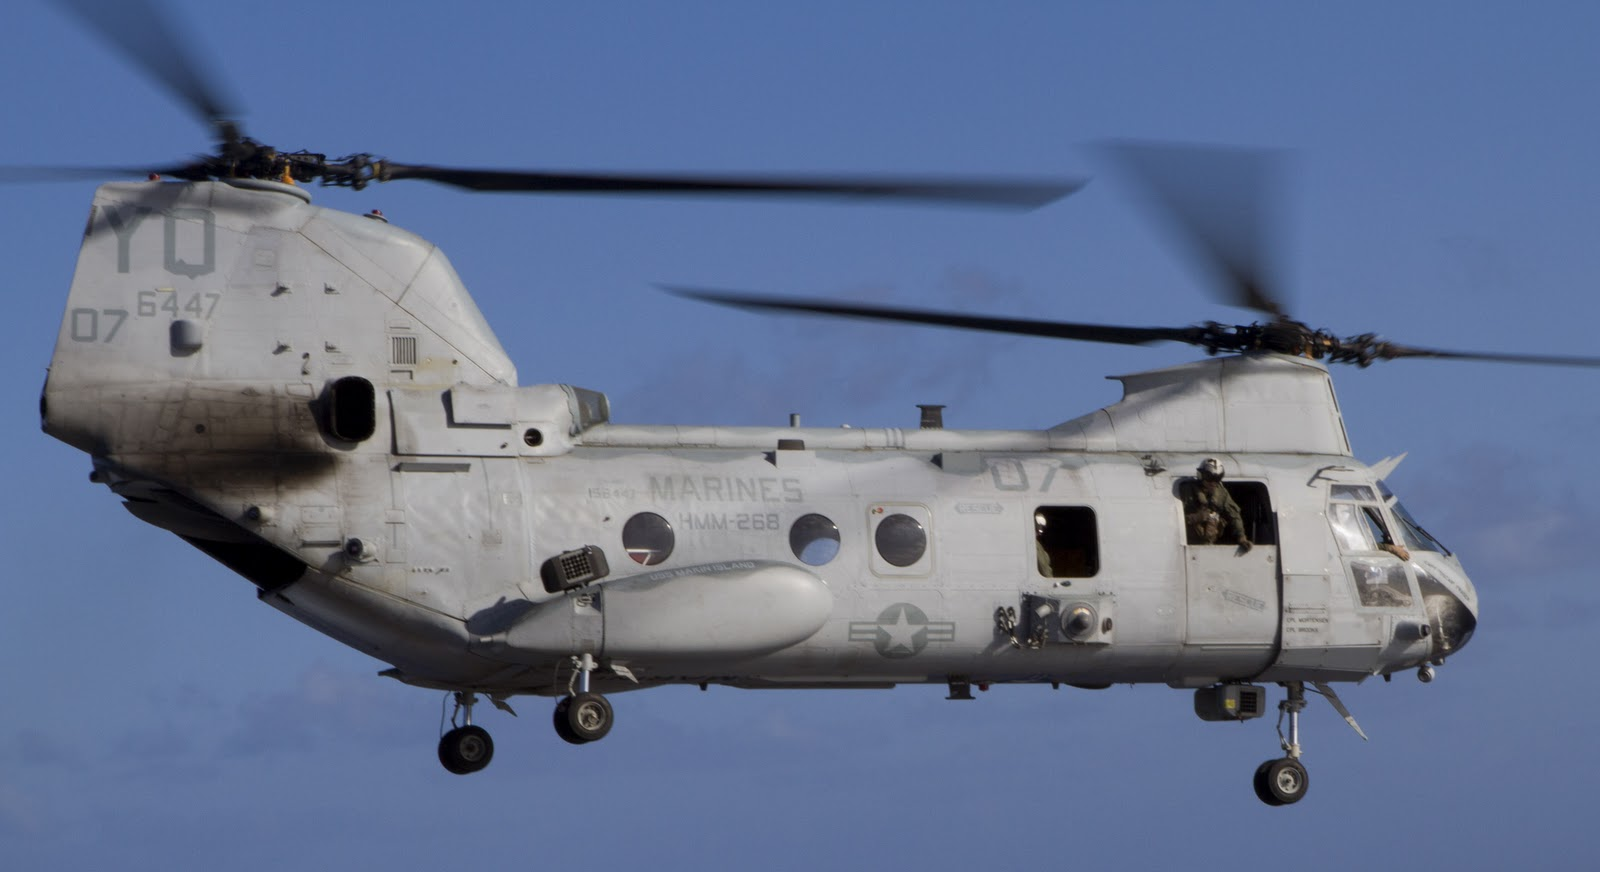
\includegraphics[height = 6cm]{Images/Literature/Tandem}     
	\caption{A military CH-46E Sea Knight, example of a typical tandem rotor}
	\label{IM_Tandem}
\end{figure}


As described in \eqref{EQ_ElectricalPowerThrust} the thrust of the system increases slower than the electrical power input into the system. In a standard configuration, doubling the electrical power would only increase the thrust by a factor of $\approx 1.587$. Where as doubling the amount of rotors being driven will double both the thrust and the electrical power. This gives the tandem arrangement the capability of lifting heavier loads with relatively low power consumption, as well as demonstrating low power consumption for hover and slow translatory flight. Having twin blades does increase the size of the craft, but the elimination of the tail rotor sees the size being similar to that of a classic helicopter.

\subsection{Multirotor Designs}
Drones have joined other remote controlled vehicles in the world of hobbyists. Of all the different designs the multirotor is the most popular. The four rotor design is generally chosen due to its incredible stability and manoeuvrability. Similar to the tandem, quadrotors have very good disk loading and thus can be used to lift heavy loads, there are even products that have 8 rotors to seriously increase the payload capability. This does however relate to a more power hungry system and a less efficient hover.

As shown in Figure \ref{IM_CounterBlades}, a quad rotor consists of two pairs of counter rotating propellers. Each shaft will be driven by its own motor and will contribute to the overall thrust and moment generation of the craft. Having the freedom to control each blade independently gives the pilot advanced manoeuvrability, with minimal mechanical complexities. This also reduces the complexity of the control algorithms as six degrees of freedom can be obtained by simply adjusting the speed of the motors. Besides the poor hover efficiency, the biggest downside of the multirotor designs is their size and weight. Each blade requires a drive system and space to rotate without interference. This generally limits the flight time of multirotors.

\begin{figure}[H]
	\centering
	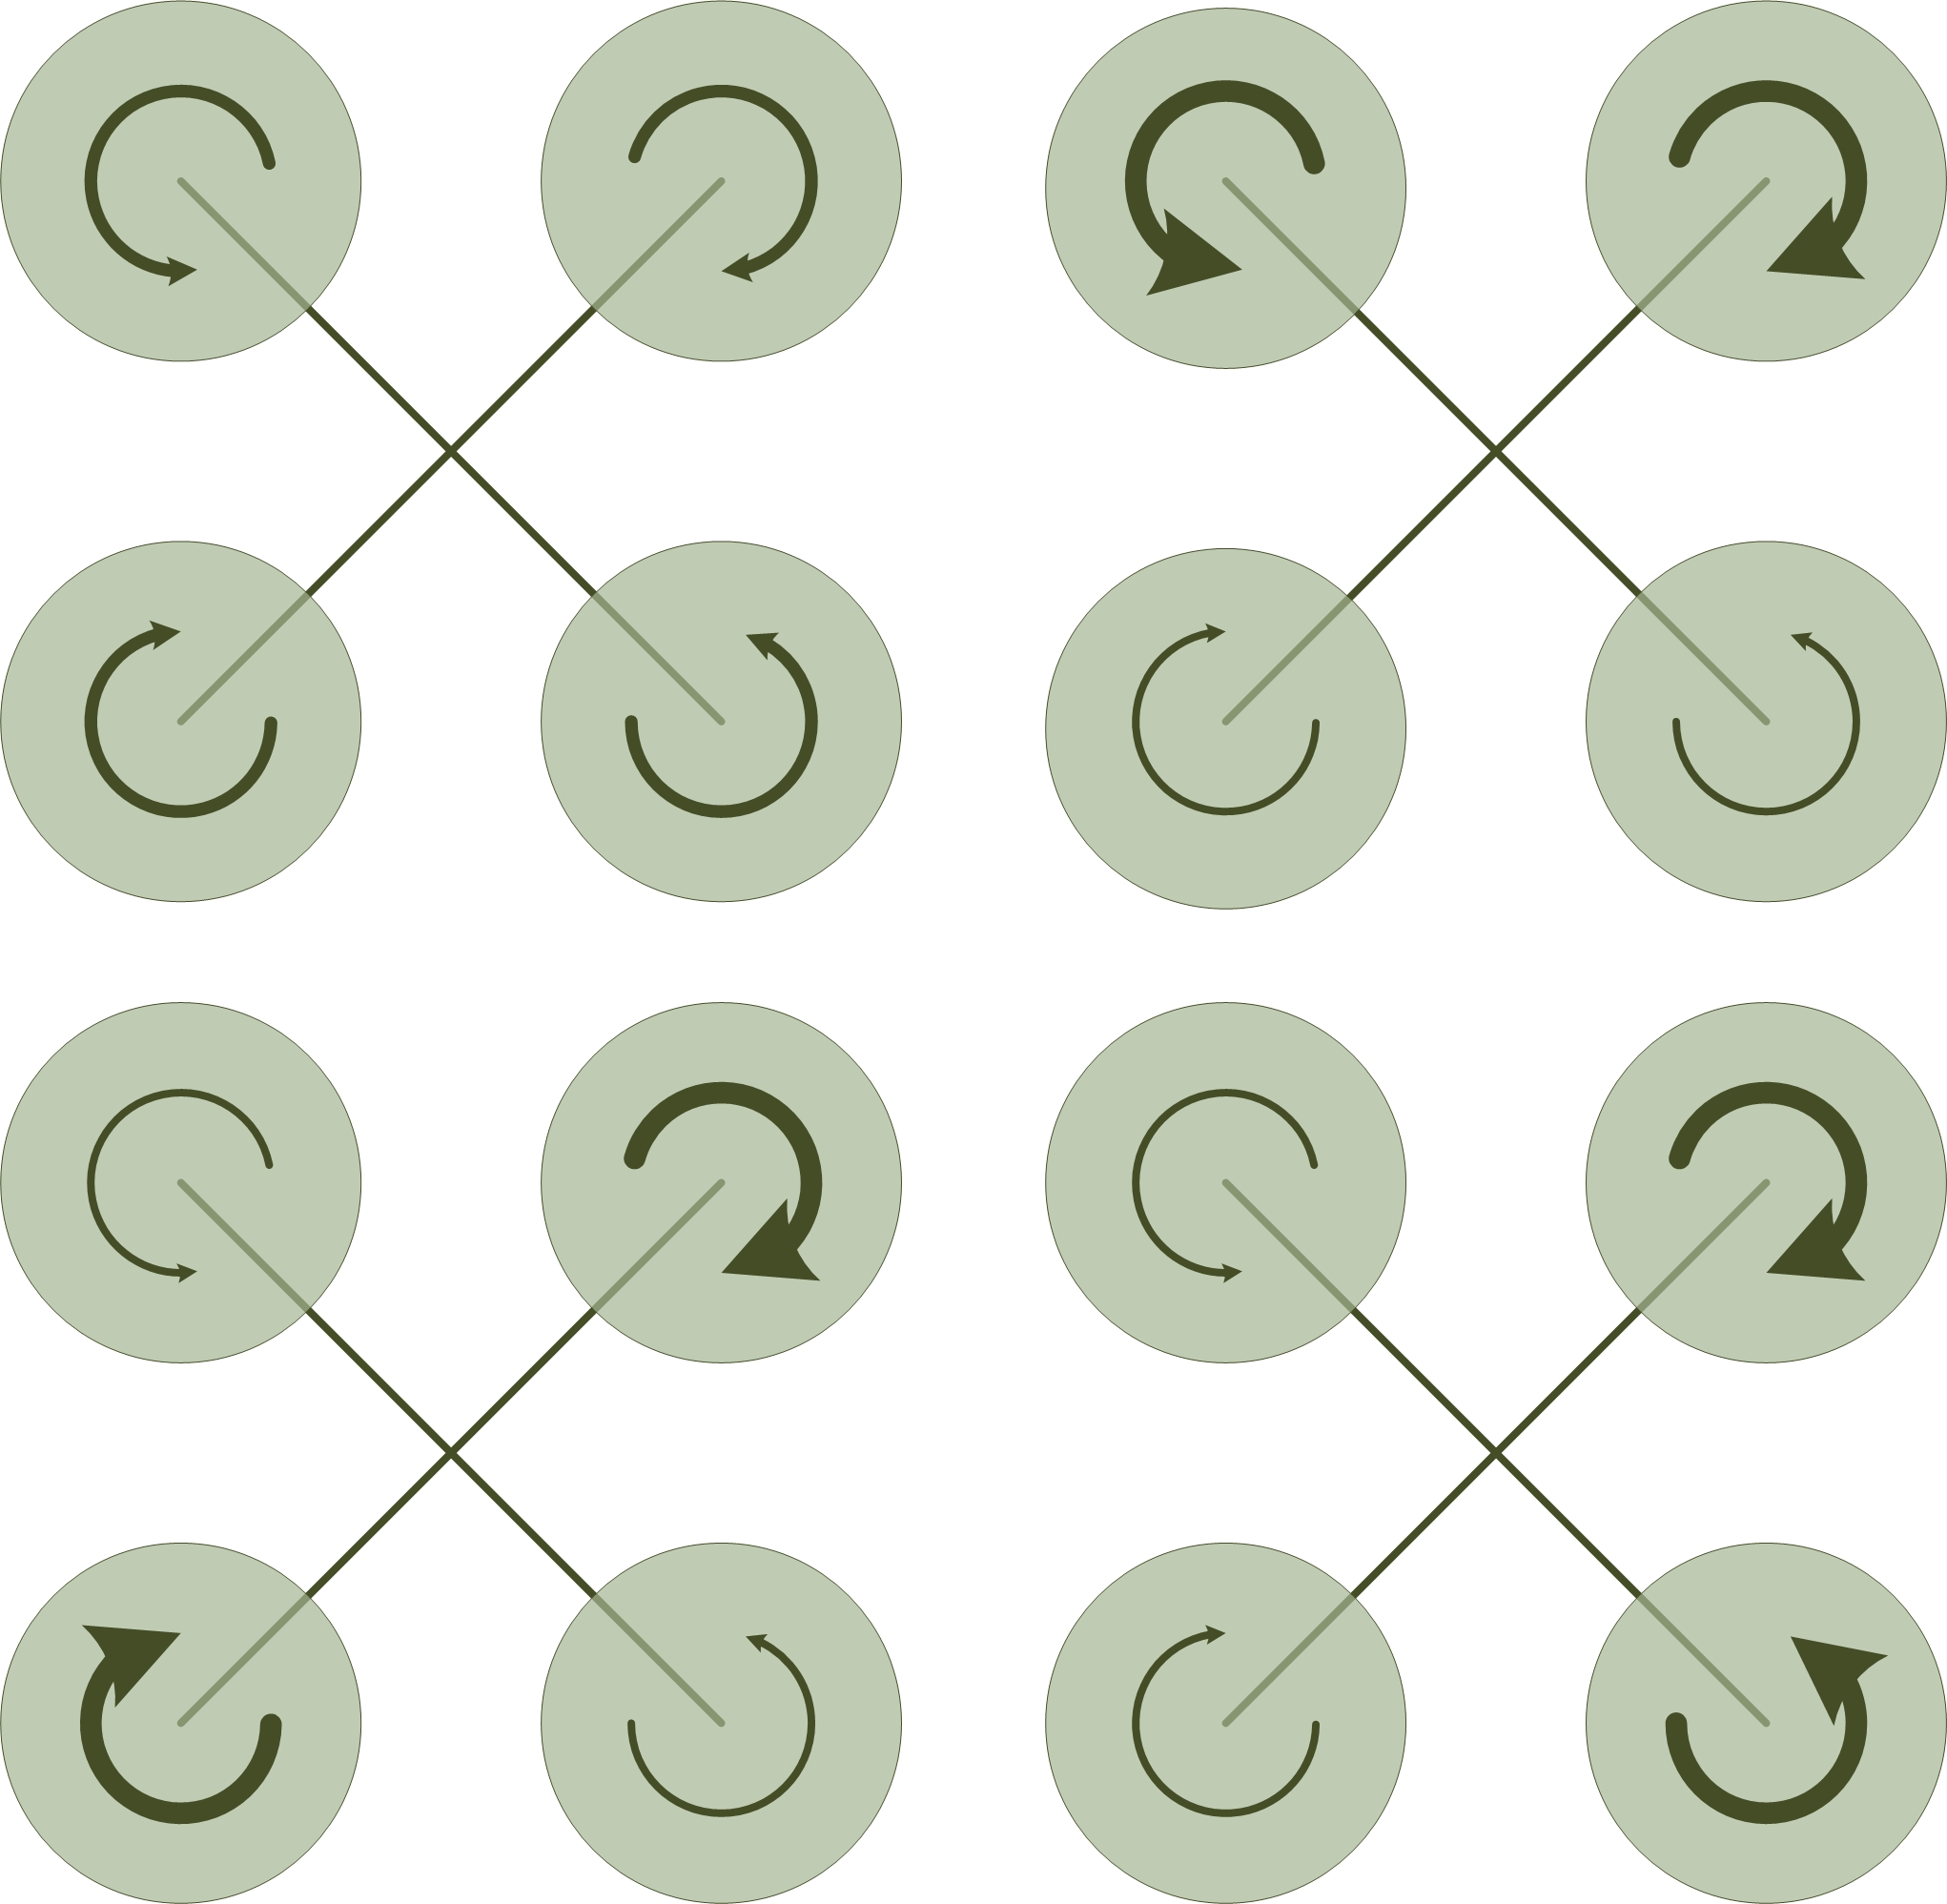
\includegraphics[height =6cm]{Images/Literature/quadrotor}
	\caption{Quadrotor configuration \cite{ThrustCritical}}
	\label{IM_CounterBlades}
\end{figure}

\subsection{Tilt Rotors}
A tilt rotor is a very sophisticated system that attempts to harness the benefits of both the fixed and rotor wing aircraft. With the addition of a pivoting axis for each blade the craft has the forward flying speeds of a fixed wing craft while still being able to take off an land vertically like a rotorcraft. The tilt rotor's major downfall is related to the required highly complex and intricate mechanical design \cite{RotorConfig}.

VTOL applications require a larger blade to decrease the disk loading, while in forward flight a smaller diameter blade is desired to increase the efficiency of propulsion. Hager \cite{US6030177} developed a telescopic system that transforms the blades to get the optimal benefits out of each configuration, shown in figure \ref{IM_TiltRotor}\footnote{(Taken from \cite{Heli})}. These and other improvements have established the tilt rotor as a competitive design in the field of aeronautic transportation \cite{RotorConfig}.

\begin{figure}[H]
	\centering
	\includegraphics[height = 6cm]{Images/Literature/TiltRotor}     
	\caption{Hager's design for a telescopic tilt rotor system \cite{Heli}}
	\label{IM_TiltRotor}
\end{figure}

\subsection{Discussion}


\section{Quadrotor Flight Dynamics}

This section will discuss some of the methods and limitations pertaining to modelling the flight dynamics of a rotorcraft. Most of the discussion will surround multirotors, specifically quadrotors, as the majority of the literature is based on these designs \cite{Luukkonen, RealTime, Pounds2006, Hoffmann, Moller2015}. Due to the mechanical complexity of swashplate designs, the discussion is assuming a fixed pitched rotor set up. 

Before control laws can be applied there must be a dynamic model of the craft. To create the model there must be a good understanding of the factors that effect these dynamics as well as the mathematical methods for deriving the equations. A brief introduction to the nomenclature and axis systems is done and is followed by a discussion into modelling rotorcraft forces and moments. After the model can be obtained mathematically it is important to discuss the physical implementation of obtaining the data, and the instrumentation required. Unfortunately its very rare to have a flying environment that is void of disturbances, this section is closed with a discussion about the various disturbances that effect the flight dynamics of rotorcraft, including some specific environmental disturbances.

	\subsection{Coordinate Systems, Rotations and Nomenclature}
	As the rotorcraft manoeuvres through space, two separate sets of axes are created. Each axis system is important and transforming easily between these frames is necessary. Some of these methods are described in this section, as well as the various means of representing these rotations. This section begins by describing these different frames, namely the inertial and body frames.
		
		\subsubsection{Inertial and Body Frame}
		The inertial, or North East Down (NED), aligns itself with the North and East directions on a compass. The third axis will align with gravity as a positive Z component. This frame assumes that the earth is flat and non-rotating and this frame's origin can be defined arbitrarily.
		
		The body frame aligns itself with the body of the drone, with the nose of the craft facing in the positive X direction and the Z axis is defined perpendicular to the rotor plane with thrust generated in a negative Z direction. The origin of the body frame is defined as the center of mass for the drone.
		
		Figure \ref{IM_Frames} is a visual representation of both frames.
		
		\begin{figure}[H]
			\centering
			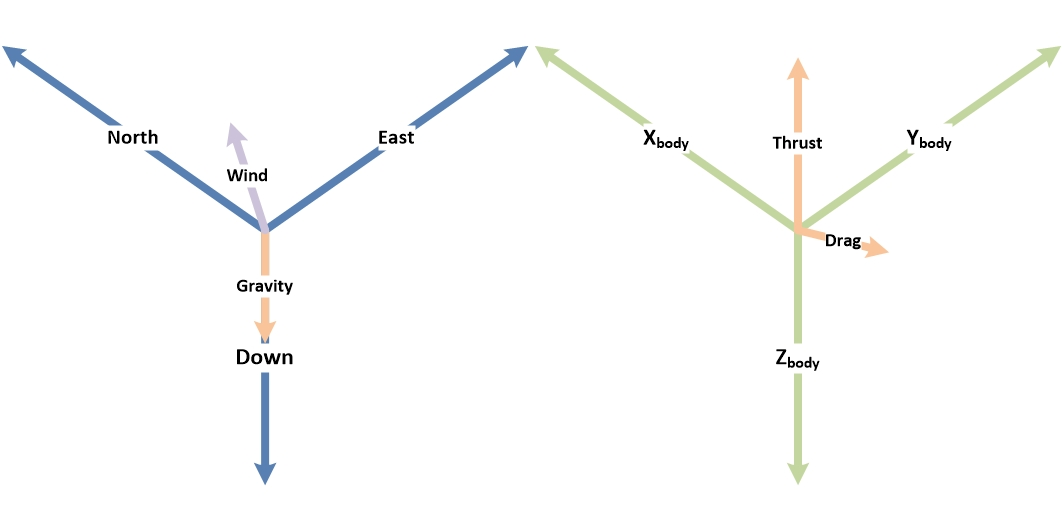
\includegraphics[height = 6cm]{Images/Literature/AxesOverlay.jpg}     
			\caption{The inertial and body frames}
			\label{IM_Frames}
		\end{figure}
			
		In order to relate the motion of the craft in the body frame to the inertial frame, it is necessary to be able to represent the rotation between these frames.
		
		\subsubsection{Euler Angles}	
		The most intuitive way to represent the rotation between two frames, is by looking at the rotation between each corresponding axis. These are known as the Euler angles and are made up of a roll ($\phi$), pitch ($\theta$) and yaw ($\psi$) angles. Euler angles provide a very intuitive understanding of the rotation between the different frames. This is best explained with Figure \ref{IM_Euler}.
		
		\begin{figure}[H]
			\centering
			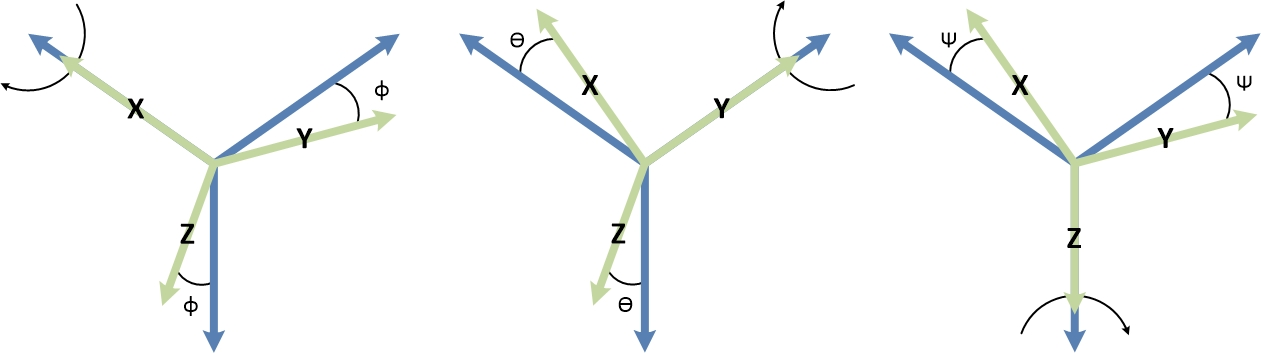
\includegraphics[height = 4cm]{Images/Literature/rotations.jpg}     
			\caption{Individual rotations around the X, Y and Z axes respectively.}
			\label{IM_Euler}
		\end{figure}
		
		The yaw angle is defined as a pure rotation around the Z-Axis. Roll and pitch are defined as pure rotations around the X-Axis and Y-Axis respectively. The Euler angle representation does have limitations, such that any 3 Euler angles could represent a different rotation, based on the order it is applied. For this project, a Euler 3-2-1 sequence will be followed. There is also a chance of a singularity at extreme angles, this is not a concern for this project, as it will only be necessary to ever complete small rotations \cite{quaternion, Moller2015}. 
		
		According to Euler's theory, any two varying coordinate axes can always be related to one another by a single rotation. 
			
		\subsubsection{Direct Cosine Matrix}
		The direct cosine matrix (DCM), provides a simple method for transforming references between two different frames. This is necessary for converting the NED frame to the body frame and vice versa. The DCM is calculated by following 3 individual rotations and multiplying their results together. A 3-2-1 Euler sequence will transform first using yaw then pitch and finally roll. Each transformation is represented as a 3x3 Matrix representing a rotation around one of the axes.
		
		In the case of rotating from the body to the NED frame, the matrix takes the form as shown in equation \eqref{EQ_RotationMatrix} \cite{Luukkonen, Moller2015} where $C_x = \cos(x)$ and $S_x = \sin(x)$. The matrix is also orthogonal, which means that $\textbf{R}^{-1} = \textbf{R}^T$. $\textbf{R}^T$ would be the rotation from the inertial frame to the body frame \cite{Luukkonen, Moller2015, quaternion}.
		
		\begin{equation}
		\label{EQ_RotationMatrix}
		\textbf{R} = 
		\begin{bmatrix}
		C_\psi C_\theta   	& C_\psi S_\theta S_\phi - S_\psi C_\phi & C_\psi S_\theta C_\phi + S_\psi S_\phi \\
		S_\psi C_\theta   	& S_\psi S_\theta S_\phi + C_\psi C_\phi & S_\psi S_\theta C_\phi - C_\psi S_\phi\\
		-S_\theta   		& C_\theta S_\phi & C_\theta C_\phi  \\
		\end{bmatrix}
		\end{equation}
		
		The DCM does provide a mathematically simple method for creating relationships between frames, however this method is computationally taxing as it is forced to recalculate the matrix and the multiplications on every loop.
		
		\subsubsection{Quaternions}
		The quaternion representation manages to minimise the computation required to calculate transformations, as well as remove the singularity found in the Euler representation \cite{quaternion}. One of the major downsides of quaternions is that they are difficult to interpret intuitively. A quaternion follows the form seen in \eqref{EQ_Quaternion} and contains a scalar value $q_w$ and a vector component $[q_x \ q_y \ q_z]$. This representation is broken up into a rotation angle, and a rotation axis.
		
		\begin{equation}
		\label{EQ_Quaternion}
		\textbf{q} = 
		\begin{bmatrix}
		q_w \\
		q_x\\
		q_y\\
		q_z\\
		\end{bmatrix}
		\end{equation}
		
		Quaternions come with their own set of mathematical rules and laws which will not discussed here. However it should noted that their are techniques that provide simple conversion from and to Euler angles and thus the DCM.  
		
		\subsubsection{Nomenclature}
		The naming convention used, follows Moller's notation \cite{Moller2015} and is shown in \ref{TAB_Nomenclature}. It makes sense that the global position and velocity of the craft be described in the NED frame, however the forces and moments will be generated in the body frame. Since there is now a simple relationship between the two frames, it is possible to relate the body frame forces and movements, into earth frame translations. The variables shown in Table \ref{TAB_Nomenclature} are visualised in Figure \ref{IM_Nomenclature}. The variables are all defined in the body frame and are shown, along with their positive directions. The right hand and thumb rule were used to dictate direction.
		
		\begin{figure}[H]
			\centering
			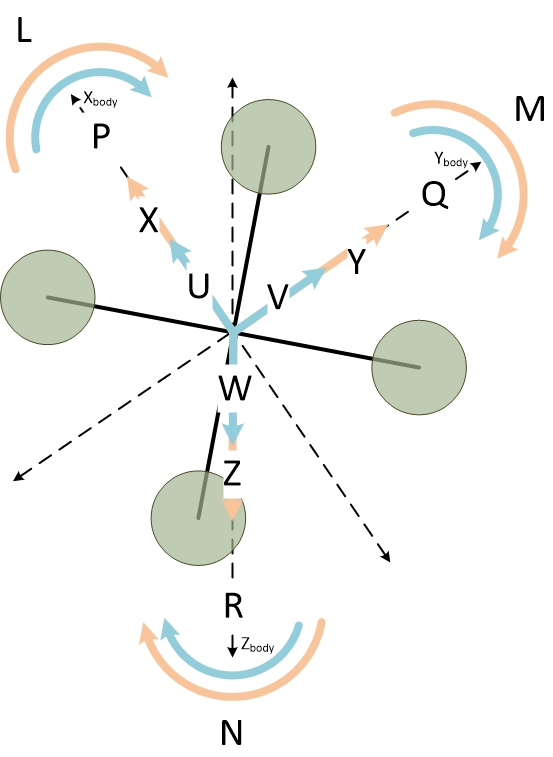
\includegraphics[height = 10cm]{Images/Literature/ForcesMoments.jpg}     
			\caption{Typical naming convention of body forces, moments and velocities for a quadrotor}
			\label{IM_Nomenclature}
		\end{figure}
		
		\begin{table}[!]
			\centering
			\begin{tabular}{| l | l |}
				X, Y, Z 	& Force vector along the respective body frame axis\\
				L, M, N 	& Moment around the respective body frame axis\\
				U, V, W 	& Linear velocity along each body frame axis\\
				P, Q, R  	& Angular velocity around each body frame axis\\
			\end{tabular}
			\label{TAB_Nomenclature}
			\caption{Standard Nomenclature}
		\end{table}
		
		The body frame forces, moments and velocities can be seen, and are described in \eqref{EQ_ForcesMomentsVelocitiesX} - \eqref{EQ_ForcesMomentsVelocitiesN}. Where X, Y, Z are the forces in each body axis, with the rotor thrust being produced in the negative Z direction. L, M, N are the moments around the x, y, z axes respectively and U, V, W are the velocities aligned with the x, y, z axes respectively. 
		
		Using the rotation matrix described in \eqref{EQ_RotationMatrix}, a relationship for North, East and Down velocities can be made and is described in \eqref{EQ_UVWtoNED}. 
		
		\begin{equation}
		\begin{bmatrix} \dot{N}\\ \dot{E}\\ \dot{D} \end{bmatrix} = \textbf{R} \begin{bmatrix} U\\ V\\ W \end{bmatrix}
		\label{EQ_UVWtoNED}
		\end{equation}
				
	\subsection{Kinetics and Kinematics}
	
	Assuming the system can be considered as a rigid body, allows for the use of normal Newtonian mechanics to create the equations of motion. This method will also use the Euler angles described above \cite{Luukkonen, Modelling, Moller2015}.
	
	The derivations of these calculations are well documented in literature \cite{Blakelock}
	
	\begin{eqnarray}
	X &=&  m(\dot{U} - VR + WQ)\label{EQ_ForcesMomentsVelocitiesX}\\
	Y &=&  m(\dot{V} - UR + WP)\label{EQ_ForcesMomentsVelocitiesY}\\	
	Z &=&  m(\dot{Q} - UQ + VP)\label{EQ_ForcesMomentsVelocitiesZ}\\
	L &=&  \dot{P}I_{xx} + QR(I_{zz} - I_{yy})\label{EQ_ForcesMomentsVelocitiesL}\\
	M &=&  \dot{Q}I_{yy} + PR(I_{xx} - I_{zz})\label{EQ_ForcesMomentsVelocitiesM}\\	
	N &=&  \dot{R}I_{zz} + PQ(I_{yy} - I_{xx})\label{EQ_ForcesMomentsVelocitiesN}
	\end{eqnarray}
	
	
	\subsection{Mass Model and the Inertia Tensor}
		\subsubsection{Mass Model}
		In any aerial vehicle mass is always an important design criterion. Every aspect of the platform must be designed to be the lightest it possibly can. Having a light weight craft is one part of the design criterion, another would be ensuring that the weight is geometrically spread out correctly, as well as functionally distributed appropriately. The table below was adapted from \cite{NewMAV} and demonstrates the latter point by showing the weight distribution of three separate crafts. Depending on the different criteria for the craft, different functional blocks will be allocated a certain percentage of weight. For example if the project requires a longer flight time, a higher percentage would be given to the power source and possibly less to the external payload. Generating a good mass model before designing helps better understand the requirements for the craft and could be a deciding factor in the construction.
		
		\begin{table}[H]
			\centering
			\begin{tabular}{l | c | c | c | c}
				
				Component 					& 0.3kg & 1.8kg & 3.7kg\\
				\hline\hline
				Rotor System 				& 11.0 & 11.2 & 13.9\\
				Tailboom Assembly 			& 8.0 & 9.1 & 7.8\\
				Main Rotor Motor 			& 15.4 & 10.5 & 8.1\\
				Fuselage/Structure 			& 7.0 &  15.1 & 12.0\\
				Main Transmission 			& 2.0 &  3.4 & 3.4\\
				Landing Gear 				& 2.3 &  3.4 & 2.9\\
				Control System 				& 5.7 & 18.3 & 9.3\\
				Avionics 						& 29.4 &  2.4 & 1.6\\
				Power Source 				& 19.2 & 26.6 & 41.0\\
				
			\end{tabular}
			\caption{MAV Weight Data (Adapted from \cite{NewMAV})}
		\end{table}
	
		\subsubsection{Inertia Tensor}
		It was also mentioned that the weight needs to be geometrically positioned correctly, the point of this would be to create as much symmetry in the craft as possible. If this is done correctly the principle axes of inertia will align very closely with the body of the craft, simplifying calculations later on and helping find and define the principle axes. The inertia tensor is a matrix that is a representation of a rigid body's resistance to rotations in 3D space. For the general case the inertia tensor takes the form as shown in equation \eqref{EQ_InertiaTensor}. The inertia tensor is very dependant on a craft's symmetry, and is symmetric itself. In other words, $I_{xy} = I_{yx}$, $I_{xz} = I_{zx}$ and $I_{zy} = I_{yz}$ and therefore if a craft is symmetric about the X, Y and Z axes, then the assumption can be made that $I_{xy} = I_{yx} = I_{xz} = I_{zx} = I_{yz} = I_{zy} = 0$ \cite{Luukkonen, MiniFlying}.
		
		\begin{equation}
		\label{EQ_InertiaTensor}
		\textbf{I} = 
		\begin{bmatrix}
		I_{xx}	& -I_{xy} & -I_{xz}\\
		-I_{yx}	& I_{yy}	& -I_{yz}\\
		-I_{zx}	& -I_{zy}	& I_{zz}\\
		\end{bmatrix}
		\end{equation}
		
		In order to successfully model a rotorcraft, the inertia tensor must be known and will be defined around the centre of rotation of that rotorcraft. The method for obtaining the inertia tensor is described in the system identification of this project.
		
	\subsection{Rotor Generated Forces and Moments}
	The forces and moments generated by the rotors are discussed here. It is assumed that the rotors will only generate a force perpendicular to their plane while the moments are dependant on the placement of the rotors.
	
	\begin{figure}[H]
		\centering
		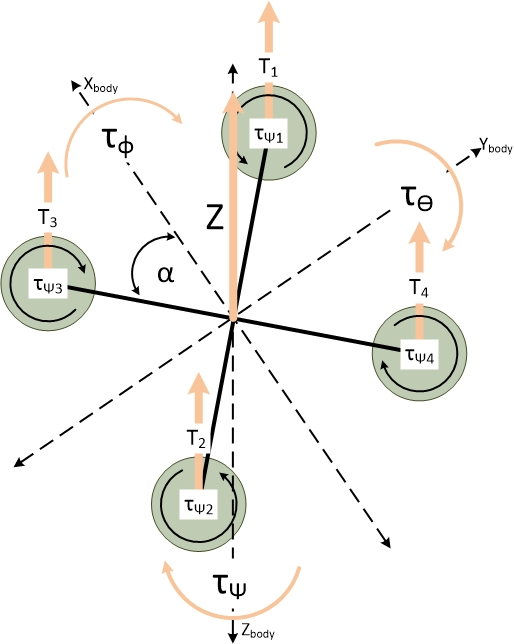
\includegraphics[height = 10cm]{Images/Literature/quadforces.jpg}     
		\caption{Forces and moments acting in the body frame on an X-Configuration quadrotor}
		\label{IM_Forces}
	\end{figure}
	
	
		\subsubsection{Actuators}
		As shown in Figure \ref{IM_Forces}, all the forces generated by the quadcopter are a product of the four rotors. The rotors convert mechanical energy from the motors into aerodynamic power. The motors convert electrical energy into mechanical energy based on the motor commands sent from the controller. Both the motors and rotors can not react instantly to new commands, this lag introduces a timing delay constant into the system \cite{Moller2015}.
		
		If the lag timing constant is defined as $\tau$, thrust generated by motor $x$ as $T_x$ and the command sent to that motor as $T_{xR}$. Then \eqref{EQ_MotorDelay} can be created and applies to all four motors.
		
		\begin{equation}
		T_x = -\dot{T_x} \tau + T_{xR}
		\label{EQ_MotorDelay}
		\end{equation}
		 		
		\subsubsection{Controlled Body Forces}
		Figure \ref{IM_Forces} assumes that all of the rotors lie in the same plane, and only provide a unidirectional force. This assumption allows the easy creation of a total force $\textbf{T}$, which is shown in \eqref{EQ_Translational} as the sum of all four motor thrusts. 
		
		\begin{eqnarray}
		Z = (T_1 + T_2 + T_3 + T_4)
		\label{EQ_Translational}
		\end{eqnarray}
		
		To command this value, a virtual actuator can be created $\delta_{Z}$ which commands all four rotor thrusts. Equation \eqref{EQ_MotorDelay} demonstrates the lag to generate these thrusts and the same lag dynamics will apply to $\delta_{Z}$, thus creating \eqref{EQ_VirtualHeave}.
		
		\begin{eqnarray}
		Z = -\dot{Z} \tau + \delta_Z
		\label{EQ_VirtualHeave}
		\end{eqnarray}
				
		\subsubsection{Controlled Body Moments}
		A quadrotor generates a moment around it's own axis through varying the speed of each motor. The torque generated is also dependant on the spacing for the type of quadrotor used. A standard X-Configuration quadrotor is shown in Figure \ref{IM_Forces} and was used for this analysis. To induce a torque around the X-axis, the sum of the two left rotors subtracted from the sum of the two right rotors must be non-zero. Similarly the front and back rotor summations must not be equal to induce a torque around the Y-axis. As shown in \ref{IM_Forces}, each rotor also creates a moment around the Z-axis. This induced torque is a product of the rotors lift to drag ratio and the chord length and is represented in \eqref{EQ_YawTorque}.
		
		\begin{equation}
		\tau_{\psi x} = \frac{r_D}{R_{LD}} \times T_x
		\label{EQ_YawTorque}
		\end{equation}
				
		Assuming that each rotor has the same characteristics and are spaced evenly, these moments can be mathematically expressed as shown in \eqref{EQ_Torques}, where $l$ is the distance from the centre of the rotor to the centre of gravity, $r_D$ is the chord length and $R_{LD}$ is the lift to drag ratio for the rotors.
				
		\begin{eqnarray}
		L &=& \frac{r_D}{R_{LD}} \times (T_3 + T_4 - T_1 - T_2)\\
		M &=& (T_1 + T_3 - T_4 - T2) \times lcos(\alpha)\\
		N &=& (T_2 + T_3 - T_1 - T4) \times lsin(\alpha)
		\label{EQ_Torques}
		\end{eqnarray}
		
		Virtual actuators can be created to command these moments, namely $\delta_\psi$, $\delta_\theta$ and $\delta_\phi$. However these commands will be subject to the same time delay experienced by the rotors. Therefore \eqref{EQ_VirtualTorquesL} - \eqref{EQ_VirtualTorquesN} can be used to represent the relationship between these commanded values and the actual moment \cite{Modelling, Moller2015}.
			
		\begin{eqnarray}
		L &=& -\dot{L} \tau + \delta_\psi\\ \label{EQ_VirtualTorquesL}
		M &=& -\dot{M} \tau + \delta_\theta\\ \label{EQ_VirtualTorquesM}
		N &=& -\dot{N} \tau + \delta_\phi \label{EQ_VirtualTorquesN}
		\end{eqnarray}
				
	
	\subsection{Disturbances}
	
		\subsubsection{Drag}
		Drag is a damping force whose quantity is relative to the speed of the object, and always opposes the direction of motion. Drag is defined here in the body frame and from \eqref{EQ_Drag} and the discussion drag, the equations for three dimensional drag can be calculated. As shown in \eqref{EQ_dragForcesX} - \eqref{EQ_dragForcesZ}, the effect of drag can be reduced through mechanical design and flight strategy, by reducing the area of the plane facing towards the direction of the motion. 
		
		\begin{eqnarray}
		F_{Dx} &=& C_{DX} (\dfrac{1}{2} \rho U^2) A_{YZ} \label{EQ_dragForcesX}\\
		F_{Dy} &=& C_{DY} (\dfrac{1}{2} \rho V^2) A_{XZ} \label{EQ_dragForcesY}\\
		F_{Dz} &=& C_{DZ} (\dfrac{1}{2} \rho W^2) A_{XY} \label{EQ_dragForcesZ}
		\end{eqnarray}
		
		Due to an offset between the centre of gravity and the centre of pressure, the drag forces can also create undesired moments. Equations \eqref{EQ_dragMomentsL} - \eqref{EQ_dragMomentsL} can be derived from the Figure \ref{IM_dragForces}, where $d_x, d_y, d_z$ are the offsets of the centre of pressure. $F_{Dx}, F_{Dy}, F_{Dz}$ are the forces generated by drag act along the coinciding body axis. $M_{Dx}, M_{Dy}, M_{Dz}$ are the and moments generated by the drag forces and the offset of the centre of pressure, they act around the coinciding axis. $A_{YZ}, A_{XZ}, A_{XY}$ are the surface areas facing the corresponding plane in the body frame with $C_{DX}, C_{DY}, C_{DZ}$ as the corresponding drag coefficients.
		
		\begin{eqnarray}
		M_{Dx} = F_{Dz} \times d_y - F_{Dy} \times d_z \label{EQ_dragMomentsL}\\
		M_{Dy} = F_{Dx} \times d_z - F_{Dz} \times d_x \label{EQ_dragMomentsM}\\
		M_{Dz} = F_{Dy} \times d_x - F_{Dx} \times d_y \label{EQ_dragMomentsN}
		\end{eqnarray}
		
		\begin{figure}[H]
			\centering
			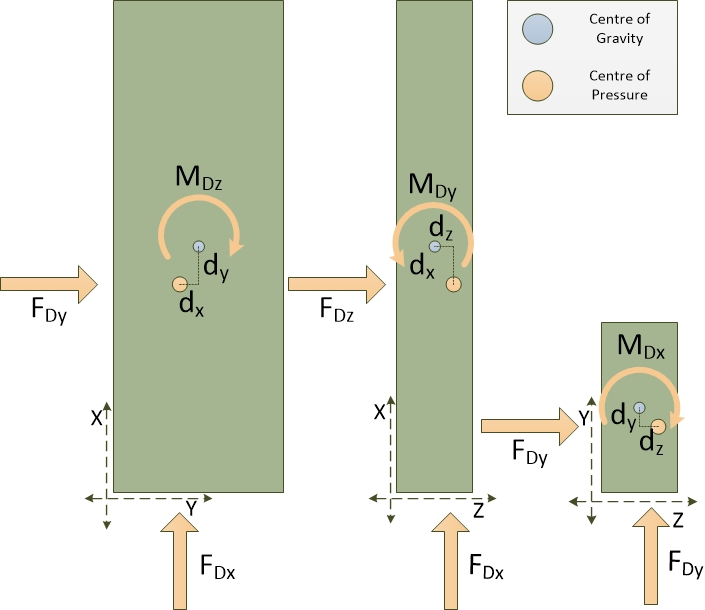
\includegraphics[height = 8cm]{Images/Literature/drag.jpg}     
			\caption{Typical moments created by drag forces}
			\label{IM_dragForces}
		\end{figure} 
				
		\subsubsection{Airflow Characteristics}
		
		In the preceding section on flight theory, the importance of air density, pressure and the creation of rotor wake boundary are discussed. The negative effects of disrupting airflow as well as the need for controlling this disturbance has been well documented in literature \cite{NearWall, Lee2012, Hoffmann}.
		
		Using Figures \ref{IM_MomentumTheoryAirFlow} and \ref{IM_MomentumTheoryHover} as references Airflow can be seen as the stream of air from $v_0$ to $v_\infty$\, through $v_i$. Equation \ref{EQ_ThrustMass} states that thrust is directly proportional to the relationship between these velocities and any deviation in these velocities will vary the thrust of the rotor in question. $v_0$ is only zero when the craft is in a state of pure hover, completely stationary, and there is no wind. Increasing the speed of the craft will increase the $v_0$ component creating a variation in the overall thrust, the same can be said for any condition that contains a tangible wind factor. 
		
		As investigated by \cite{Hoffmann} mechanical intrusions will have an effect on the far wake velocity, thus also effecting the generated thrust. In the design of STARMAC by Hoffmann et al \cite{Hoffmann} the frame was designed to be very configurable so that the effects of the mechanical design could be quantified. Originally the rotors were shrouded and quite close to the centre of gravity of the craft. The shrouds were a distance of 5\% rotor radius and when removed the yaw tracking improved from $\pm$10\textdegree to $\pm$3\textdegree. When not included in the dynamic model the obstruction in the air stream will cause lower and less stable values of thrust, affecting the accuracy of the model. 
		
		When the rotors were located close to the centre of gravity they obtained some attitude disturbances that were eliminated by moving the rotors further away. It was also observed that any object that lies close to the rotor tip, created intense arbitrary disturbances and should be avoided \cite{Hoffmann}.
		
		\cite{NearWall} attempts to model some of the disturbances for a single rotor craft hovering near wall, but as stated by \cite{Lee2012} it is not viable to accurately quantify these disturbances, however their presence must not be neglected. As Figure \ref{IM_NearWallF} shows, these can be modelled as a disturbance to the input force and moments.
		
		\begin{figure}[H]
			\centering
			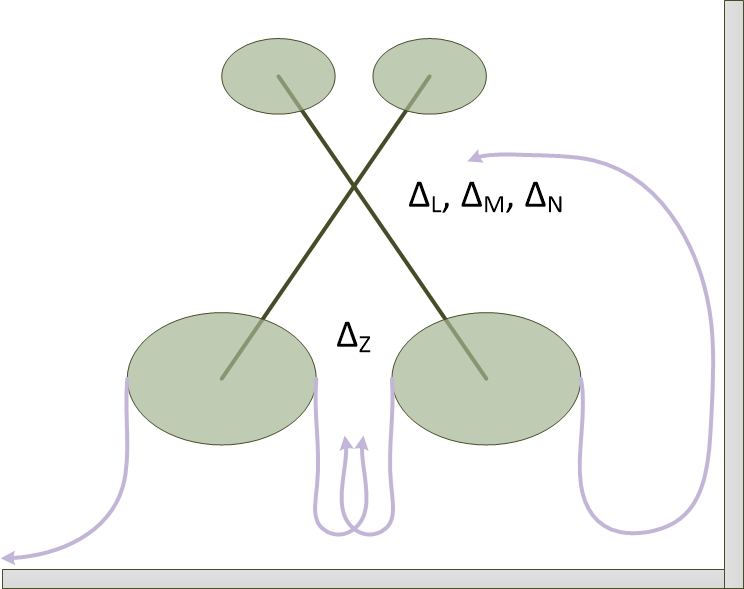
\includegraphics[height = 7cm]{Images/Literature/near_wall}     
			\caption{Velocity components though the rotor for, no wall (left) and near wall (right) conditions (Taken from \cite{NearWall})}
			\label{IM_NearWallF}
		\end{figure}
		
		As demonstrated by \cite{NearWall}, there is also an induced moment acting on the rotor as the rotor approaches the wall. Figure \ref{IM_NearWall} is an image generated by \cite{NearWall}, it demonstrates the change in airflow on a rotor close to a wall region.
		
		\begin{figure}[H]
			\centering
			\includegraphics[height = 5cm]{Images/Literature/NearWall}     
			\caption{Velocity components though the rotor for, no wall (left) and near wall (right) conditions (Taken from \cite{NearWall})}
			\label{IM_NearWall}
		\end{figure}
		
		In \cite{NearWall}, Robinson et al used the script $c$ as their unit of measure for distance to the wall, $c$ is chord length of the airfoil. The graph shown in Figure \ref{IM_NearWallGraph} shows how the moment felt by the craft varies with the distance to the wall. The direction of the moment will be perpendicular to the wall. As above, this disturbance can also be modelled as a variation to the input moments to the system.
		
		\begin{figure}[H]
			\centering
			\includegraphics[height = 5cm]{Images/Literature/NearWallGraph}     
			\caption{Graph showing relationship between distance from the wall and moment felt be the craft (Taken from \cite{NearWall})}
			\label{IM_NearWallGraph}
		\end{figure}
		
		In \cite{NearWall} they conclude their paper by describing a proposed method of control which will be investigated further in this text. This dynamic flight model requires sensing of specific craft variables, typical sensing methods and requirements are discussed in the proceeding section. 
	
	\subsection{Instrumentation}
	The need for a well instrumented craft is intuitive and well documented in literature \cite{Moller2015, Hoffmann}. With modern advancements in sensing technology there is now a number of methods to obtain the required information. However, some of these are very costly and require specific operational environments. For this purpose, only the inertial measurement unit (IMU) and the global positioning system (GPS) are discussed here.
	
		\subsubsection{Inertial Measurement Unit}
		Traditionaly an IMU will consist of an accelerometer, gyroscope and possibly a magnetometer. The accelerometer has the ability to measure accelerations in the body axis. It should be noted that an accelerometer in rest, sitting along the inertial axis will provide a reading of $[0\  0\  g]^T$. The gyroscope measures the rotational accelerations of the craft, thus measuring 6 degrees of freedom in total. Unfortunately gyroscopes suffer from sensor drift and needs compensation. The accelerometer's gravity offset can be used to align with the vertical axis, however a magnetometer is required to account for drift in the horizontal plane. Various filtering and fusion techniques are used to combine these readings, the most popular of which  is a Kalman Filter \cite{Moller2015, Hoffmann}.
		
		\subsubsection{Global Positioning System}
		The most common method of measuring a drone's position is with the use of a GPS. The GPS readings can also be used to create an estimate of the craft's linear velocity in the inertial frame. When combined, multiple GPS unit's can be used to obtain higher precision. A major downside of a GPS is the dependence on a satellite link, this dependence severely limits the operational environments for this sensor. Other methods of localisation include using known maps and proximity sensing to provide the rotorcraft with position estimates. As discussed, these techniques are out of scope for this project and will not be considered. This project will assume an earth position and velocity estimate are present, subject to filtered noise provided through band limited white noise \cite{Moller2015}
		
		\subsubsection{Measurement Noise}
		From the discussion it is evident that sensors will not be without error. The noise associated with the measurements will be different for both varying sensor types and manufacturers and will depend on the chosen sensors. The characterisation of the noise for this project is discussed in the system identification chapter. The environment in which these sensors operate also has a significant effect on operation. Moller characterises this measurement noise as a random band limited white noise block. and adds a low pass filter to the GPS measurements \cite{Moller2015}.

\section{Collision Protection Techniques}
	\todo[inline]{Need to decide if I should keep this in,l and in what format}
	\cite{Klaptocz2013, Collision, Klaptocz2012, Briod2012, Daler2013, Klaptocz2010}
	\subsection{Impact Resistance}
	%Refer to impulse equations, Newtons's laws
	%look at car designs
	Impact resistance is a technique used by a variety of fields in the world today. Included in this is something as simple as the shocks or suspension in a car, they are designed to allow the automotive to withstand sudden impacts. Generally these techniques use a component that has some tangible spring constant.
	
	
	\subsection{Rolling Cage}
	\todo[inline]{Although a lot can be learnt from this design in terms of collision resistance, for the proposed end use case the design will not be pursued. The rolling cage design}
	
\section{Review of Existing Flight Control Strategies}\label{SECT_ControlReview}
The object of this section is gain a better of understanding of successful controller designs. Moller's control structure was used as a basis for this section \cite{Moller2015}. A simplified block diagram is shown in Figure \ref{IM_ControlOverviewSimplified}. The open source software framework, ArduPilot is a well developed code base. The quadrotor code was also reviewed to establish an understanding of implementing these 

 Along with an analysis of an existing open-source framework. For a fully autonomous vehicle, the controller would need to include multiple control loops.

This section begins with
\begin{figure}[H]
	\centering
	\includegraphics[height = 6cm]{Images/Literature/TiltRotor}     
	\caption{Hager's design for a telescopic tilt rotor system \cite{Heli}}
	\label{IM_ControlOverviewSimplified}
\end{figure}

The high level control structure can be decomposed into 
		
	\subsection{Altitude Control System}
	
	\subsection{Heading Control System}
	
	\subsection{Horizontal Control System}
	
	\subsection{Disturbance Based Observer Controller}\label{SectionDisturbanceObserver}
	Discuss and explain generic disturbance based observer stuff. In the control section discuss specific implementation. Mention standard equations here. 
	
	
\section{Collision Avoidance Techniques}

	\subsection{Sensing Techniques and Requirements}
	
		\subsubsection{Modelling}
		
	\subsection{Potential Field Method}
	
	
	
	
	
	
	
	
	
	
	
	
	
	
	

%\chapter{System Design Description}
The following chapter gives an overview behind the system design of \projectName. The chapter begins by working through the hardware system architecture diagram shown in Figure \ref{IM_SystemArchitecture}. The first consideration is the size and mounting needs of the system, provided by the mechanical platform. This gives a good start to elaborate on the needed capabilities of the proposed method of propulsion. The next considerations are the electronic modules required to run all the necessary peripherals. Finally, to interface all these blocks together will require both software and control architectures. This chapter will discuss the requirements for each section and expand on how the interfacing for the entire system will function.

	\section{System Hardware Architecture}
	The system architecture for \projectName is laid out below in Figure \ref{IM_SystemArchitecture}. The hardware system comprises of 3 main subsystems, namely Mechanical Construction, Propulsion and Electronics. The role each subsystem plays in meeting the system requirements is discussed in more detail below.
	
	\begin{figure}[H]
		\centering
		\includegraphics[height = 10cm]{../Design/System/SystemArchitecture/SystemArchitecture.jpg}
		\caption{System Architecture}
		\label{IM_SystemArchitecture}
	\end{figure}
		
		\subsection{Platform Construction}
		The platform is the physical embodiment of the craft. In this context this includes the mechanical construction of the craft, as well as the flight generating components.
		
			\subsubsection{Mechanical Construction}
			The mechanical construction of the system introduces size restrictions for the rest of the system. It should provide adequate mounting for the necessary peripherals described in the sections following. The structure needs to protect the rotors from collisions be means of a shroud and include lightweight landing gear. The chassis must also be such that the weight is distributed as symmetrically as possible. The propulsion system must be housed and provided with rigidity for steady flight control.

			\subsubsection{Propulsion and Flight Characteristics}
			The propulsion system comprises of the motors and propellers. This subsystem needs to supply enough thrust and overhead for steady control, as well as enough lifting capacity to carry any additional, mission sensors. The craft should be able to handle a \payLoadMass payload. To ensure capable disturbance rejection, the total maximum thrust should be no less than $150\%$ of hover.
			
			The craft must efficiently hover and fly at low speeds. The craft should have multiple control surfaces to accurately counter disturbances. Due to the intended use case, the craft will fly with a set orientation and thus does not require the abilities for sharp turns of manoeuvres.
		

		\subsection{Electronics Interface}
		At the core of any reliable robotic platform is a thoroughly planned electronics system, for \projectName this is the most complex subsystem containing the most modules. It is responsible for all intelligence and power generation. This subsection breaks this subsystem into more discrete parts. It begins by separating the two computing modules into real time and non-real time components. The real time components include some of the on board sensors which are required for stable and fast control theories, which all feed into the flight controller. For the drone to successfully navigate an environment it will need to better understand it's surroundings. The flight controller will analyse this data and based on flight software will control the electronic speed controllers. The on board computer will process and handle all non flight critical sensor information and can be considered as the mission computer. The OBC must also have provision to connect to a sensor pack via a predetermined interface. Another useful and necessary function, will be the ability to illuminate a dark area. 
		
		The network design will also consist of 2 discrete wireless links. Each link is dedicated to one of the computing modules. The real time node will be interfaced through a low bandwidth, high range and high reliability interface. With the non-real time node linking to the high bandwidth interface which will have lower range and reliability requirements. Both of these interfaces will link to a ground station of some sort.
		
		No system can operate without a sufficient power source. In the case of any robotic system it is important that every aspect of the design is optimised. To assist with that an electrical analysis is done to help pinpoint some of the major power consuming components. This analysis will also help to evaluate the required power source. The capacity of the power supply is limited by weight and should be optimised to the lifting capacity of the platform. Once the battery chemistry has been decided upon, work can be done to design a robust power management system. Limiting the leakage of every subsystem as well as choosing efficient modules are both part of an effective power management system. To complete the subsystem will require some form of power monitoring as well as an efficient charging scheme.
		
			\subsubsection{Flight Controller}
			The flight controller is responsible for handling all the flight critical sensor data. Using a mixing algorithm it will then output signals to the electronic speed controllers. There are multiple options for flight controllers, all tailored to different applications, platforms and flying styles. Each option has there own level of reconfigurability. For this application it is important that the chosen flight controller allows access to both the inner control loops as well as allows additional sensor data to be added into the architecture. The flight controller is also responsible for handling the pilot commands sent via the radio link, as well as transmitting in flight diagnostic information back to the ground control station.
				
			\subsubsection{Electronic Speed Controller}
			The flight controller will take in information from some of the on board sensors. It then sends a motor control command based on that information to the electronic speed controller (ESC), which directly controls the speed of each motor. This part needs to be chosen based on the maximum amount of current it can handle. At 100\% throttle the current draw of the motor should not exceed 75\% of the ESC's limit. Another important consideration is the ESC's refresh rate and computing speed. The flight controller will be rapidly sending data to the ESC. The quicker the module can respond, the more accurately the platform will fly. 
			
			Each ESC has built in intelligence and will have their own dedicated firmware. Most ESCs will come with built in firmware, which must be tailored for a quadcopter configuration.
			
			\subsubsection{On Board Computer}
			Where the flight controller ensures the craft maintains steady flight, the On Board Computer (OBC) handles all higher level processing. This will include interfacing to the rest of the on board sensors, the sensor pack as well as handling the high bandwidth networking. The OBC should not be required for flight purposes, and can thus be considered as a dedicated mission computer. 
			The OBC should be as light weight as and low power as possible. The OBC must be sufficiently powerful to do real time analysis of camera data. The OBC must have multiple communication ports to easily interface to other sensors.
					
			\subsubsection{Networking}
			This subsystem will handle control commands, flight and diagnostic data or real time sensing information. As described above these have been separated into two distinct categories, low and high bandwidth or alternatively named as high and low range. 
			
				\paragraph{Low Bandwidth, High Range}
				A reliable connection is an important factor to ensure a successful mission the hardware will be validated against it's range, speed, packet loss and ultimately reliability.
						
				The design will incorporate multiple communication peripherals as a fail-safe in case communications are lost to the base station. The pilot needs full control through it and any relevant data that needs to be transmitted will be sent here as well.
						
				\paragraph{High Bandwidth, Low Range}
				The higher bandwidth connection will be used for higher level mission control and data. The high bandwidth link should be able to transmit large streams of data between the craft and the ground control station. 
			
			\subsubsection{On Board Sensors}
			
			\subsubsection{Sensor Pack}
			The actual sensor pack in question will remain generic. So that the platform can cater for an array of sensing devices and applications. To ensure compatibility, the sensor pack needs to be able to powered as well as communicated to. It will have access to interface directly to the OBC.
	
			\subsubsection{Power Supply}

				
	\section{System Software Framework}
	The electronic components gather and collect all the necessary information, the software combines it all and controls the flow of data to obtain stable flight and more. The software system can also be broken down into different operational groups or subsystems. These are, the firmware running the flight controller, the communication protocols used between the software nodes as well as the ground control station. The ground control station although not deployed on the platform, is still mission critical and must be able to display in flight data and send commands to the craft. The last module is the logging and simulation node, which allows for an in depth understanding of untested flight dynamics.
	
		\subsection{Flight Controller Firmware}
		Most commercial flight controllers will come preprogrammed with flight control software. The required firmware blocks are represented in Figure \ref{IM_SoftwareArchitecture} and are discussed in the subsections that follow.
		
		\todo[inline]{Make figure and add in the blocks required}
		\begin{figure}[H]
			\centering
			\includegraphics[height = 4cm]{../Design/Software/FirmwareBlocks}
			\caption{Software Framework}
			\label{IM_SoftwareArchitecture}
		\end{figure}
		
			\subsubsection{Flight Modes}
			All the different modules must be accessible and configurable. The flight controller must be able to handle different flight modes that can be changed during a mission. There must be an autonomous flight mode, where the craft can follow set way points. When not in autopilot, the pilot must be able to send the craft commands to control it's movement. 
			
			\subsubsection{Position Controller}
			For precise control, the firmware will need both a well defined position and attitude estimator. 
			The position estimator must accurately predict the current position of the craft and accept new set points based on user defined way points. 
			The position control must create angle and throttle commands to rectify the error calculated in the position estimator. The commands are then sent to the attitude estimator to create new attitude set points. 
			
			\subsubsection{Attitude Controller}
			The attitude estimator must measure the crafts orientation and will be fed information from both the on board positioning monitoring system, as well as the inertial measurement unit. The attitude estimator must be able to take new set points from either the user or the position controller, depending on flight mode. The set points are then fed into the attitude control which calculates the error and generates PWM motor commands that are sent to the ESCs.
			
			\subsubsection{Way Point Navigation}
			As mentioned, the controller must have a way points navigation module, that can feed new position commands into the position estimator. The way points module will need to be able to update during a mission. The way points become the mission goal, to obtain this goal in a confined space, the craft must be able to deviate off course to avoid obstacles. 
			
			\subsubsection{Proximity Sensing}
			Obstacle avoidance calls for a module that can calculate the craft's proximity to it's immediate surroundings. This module will accept information from proximity sensors and output warnings to the position control. The position control must generate a flight strategy that allows for deviations off course, while the total deviation must round to zero.
					
		\subsection{Communication Protocols}
		The communication to and from the craft is represented in \ref{IM_SystemArchitecture}.
			\subsubsection{Radio and Telemetry}
			The radio frequency (RF) must be \todo{insert South African regulation frequency}. This link is a higher range connection and must be able to send commands reliably to the craft. 
			The telemetry link is between the GCS and the craft. It is a higher bandwidth connection and must be able to send in flight data and receive commands from the GCS. More is specified in the ground control software section.
			\subsubsection{Mission Computer}
			\subsubsection{External Sensors}
		\subsection{Ground Control Software}
		The ground station must deploy software that can visualise flight data. The GCS must also be able to send commands to the craft as well as update the mission plan.
			\subsubsection{Data Visualisation}
			\subsubsection{Basic Commands}
			\subsubsection{Way Points}
		\subsection{Logging and Simulation}
		Flight data must be collected and accessible for interpretation and graphing. New strategies can be developed from this data and tested by simulating certain aspects of the hardware.
			\subsubsection{Graphing}
			\subsubsection{Simulation in the Loop}
			\subsubsection{Hardware in the Loop}			
		







					
\chapter{Platform Design}
This chapter contains the details of physically designing a quadcopter for use in a confined space. The hardware design decisions are preceded by giving an overview of the total system design. After the high level design has been done, this chapter looks into different platform designs and rotor configurations. Based on empirical data analysis and knowledge learnt through an analysis of conventional rotors in Section \ref{SECT_RotorConfig}, the best suited rotor configuration is identified. Once a suitable platform has been chosen, a look into the required electronics is done. This includes all the electronics required for stable flight, as well as sensor requirements for operations and flight strategy. The chapter is concluded with a summary of the platform decisions made and used in the simulation.

The final design will be modelled and used to validate the proposed outcomes for this work. Although this chapter will discuss the various aspects of a quadrotor, it will focus on the components required for creating an accurate simulation of the system.

	\section{System Hardware Architecture}
	The following section gives an overview behind the system design of \projectName. The section begins by working through the hardware system architecture shown in Figure \ref{IM_SystemArchitecture} and identifying the objectives and roles of each subsystem in the design. The first consideration is the size and mounting needs of the system, provided by the mechanical platform. This gives a good start to elaborate on the needed capabilities of the proposed method of propulsion. The next considerations are the electronic modules required to run all the necessary peripherals and obtain all the required sensor data.
	
	The system architecture for \projectName is laid out below in Figure \ref{IM_SystemArchitecture}. The hardware system comprises of 3 main subsystems, namely Mechanical Construction, Propulsion and Electronics. The role each subsystem plays in meeting the system requirements is discussed in more detail below.
	
	\begin{figure}[H]
		\centering
		\includegraphics[height = 15cm]{../Design/System/SystemArchitecture/SystemArchitecture.jpg}
		\caption{System Architecture}
		\label{IM_SystemArchitecture}
	\end{figure}

		\subsection{Platform Construction}
		The platform is the physical embodiment of the craft. In this context this includes the mechanical construction of the craft, as well as the flight generating components.
		
			\subsubsection{Mechanical Construction}
			The mechanical construction of the system introduces size and weight restrictions for the rest of the system. It should provide adequate mounting for the necessary peripherals described in the sections following, while remaining as light weight as possible. The structure needs to protect the rotors from collisions be means of a protective shroud and include lightweight landing gear. The chassis must also be such that the weight is distributed as symmetrically as possible. The propulsion system must be housed and provided with rigidity for steady flight control.
			
			\subsubsection{Propulsion and Flight Characteristics}
			The propulsion system comprises of the motors and propellers. This subsystem needs to supply enough thrust and overhead for steady control, as well as enough lifting capacity to carry any additional, mission sensors. The craft should be able to handle a \payLoadMass payload. To ensure capable disturbance rejection, the total maximum thrust should include sufficient overhead above the hover requirement.
			
			The craft must efficiently hover and fly at low speeds. The craft should have multiple control surfaces to accurately counter disturbances. Due to the intended use case, the craft will fly with a set orientation and thus does not require the abilities for sharp turns of manoeuvres.	
		
		\subsection{Electronics Interface}
		At the core of any reliable robotic platform is a thoroughly planned electronics system, for \projectName this is the most complex subsystem containing the most modules. It is responsible for all intelligence and power generation. This section breaks this subsystem into more discrete parts. It begins by separating the two computing modules into real time and non-real time components. The real time components include some of the on board sensors which are required for stable and fast control, which all feed into the flight controller. For the drone to successfully autonomously navigate an environment, it will need to better understand it's surroundings. The flight controller will analyse this data and based on flight software will control the electronic speed controllers (ESCs). The on board computer (OBC) will process and handle all non flight critical sensor information and can be considered as the mission computer. The OBC must also have provision to connect to a sensor pack via a predetermined interface. Another useful and necessary function, will be the ability to illuminate a dark area. 
		
		The network design will also consist of 2 discrete wireless links. Each link is dedicated to one of the computing modules. The real time node will be interfaced through a low bandwidth, high range and high reliability interface. With the non-real time node linking to the high bandwidth interface which will have lower range and reliability requirements. Both of these interfaces will link to a ground station of some sort.
		
		No system can operate without a sufficient power source. In the case of any robotic system it is important that every aspect of the design is optimised. To assist with that an electrical analysis is done to help pinpoint some of the major power consuming components. This analysis, along with a required flight time, will also help to evaluate the required power source. The capacity of the power supply is limited by weight and should be optimised to the lifting capacity of the platform. Once the battery chemistry has been decided upon, work can be done to design a robust power management system. Limiting the leakage of every subsystem as well as choosing efficient modules are both part of an effective power management system. The analysis of the power system is important since it generally contributes a very high percentage to the overall mass of the craft.
		
			\subsubsection{Flight Controller}
			The flight controller is responsible for handling all the flight critical sensor data. Using a mixing algorithm it will then output signals to the electronic speed controllers. There are multiple options for flight controllers, all tailored to different applications, platforms and flying styles. Each option has there own level of reconfigurability. For this application it is important that the chosen flight controller allows access to both the inner control loops as well as allows additional sensor data to be added into the architecture. The flight controller is also responsible for handling the pilot commands and waypoints sent via the radio link, as well as transmitting in flight diagnostic information back to the ground control station.
			
			The flight controller's computing time capabilities have a direct influence on the system. This timing needs to be understood and introduces requirements on the controller designs. Any additional computing the craft needs should be handled by the OBC and not the flight controller. This will reduce the risk of unmodelled timing delays and unrealistic controller design goals.
			
			\subsubsection{Electronic Speed Controller}
			The above mentioned flight controller sends a motor control command based on gathered and calculated information to the electronic speed controller (ESC). The ESCs then in turn directly control the speed of each motor. Each motor should have a dedicated ESC. This part needs to be chosen based on the maximum amount of current it can handle. At $100$\,\% throttle the current draw of the motor should not exceed $75$\,\% of the ESC's limit. Another important consideration is the ESC's refresh rate and computing speed. The flight controller will be rapidly sending data to the ESC. The quicker the module can respond, the more robustly the platform will be controlled. Possible timing delays can be accounted for by ensuring the controller have sufficient phase margins. 
			
			Each ESC has built in intelligence and will have their own dedicated firmware. Most ESCs will come with built in firmware, which must be tailored for a quadcopter configuration.
			
			\subsubsection{On Board Computer}
			Where the flight controller ensures the craft maintains steady flight, the On Board Computer (OBC) handles all higher level processing and flight strategy. This will include interfacing to the rest of the on board sensors, the sensor pack as well as handling the high bandwidth networking to the ground station. The OBC should not be required for flight purposes, and can thus be considered as a dedicated mission computer. 
			The OBC should be as light weight and low power as possible while being sufficiently powerful to do real time analysis of camera data for future missions. The OBC must have multiple standard communication ports to easily interface to other sensors. There should also be a highly reliable, and fast interface between the OBC and the flight controller, thus allowing more complex flight strategies to be put in place, while not risking the robustness of the tracking control.
		
			\subsubsection{On Board Sensors}
			The on board sensors can be split up into two distinct categories. The first set of sensors are to enable stable flight of the craft and are used to close the control loops. Examples of such sensors would be inertial measurement units (IMU), global positioning units (GPS) and other relative velocity measuring sensors. 
			
			The second set of on board sensors are required for enabling more intelligent autonomous flying strategies. Examples of these sensors include proximity measurements to enable obstacle avoidance and localisation. Other types of sensors from this set could include condition monitoring of the craft's batteries. 
		
			\subsubsection{Sensor Pack}
			The actual sensor pack in question will remain generic. So that the platform can cater for an array of sensing devices and applications. To ensure compatibility, the sensor pack needs to be powered and communicated to. It will have access to interface directly to the OBC. Typical examples of sensor pack application would be mapping equipment and stored video feed for post flight inspections.
		
	\section{Platform Construction}			
		\subsection{Factors Affecting Design Decisions}
		\todo[inline]{not sure about the name of this section}
		Before a proper analysis can be done, specific design criteria need to be outlined. These include aspects of the project such as the required flight time and manoeuvring decisions. These factors have been drawn up from the proposed research questions and end use case.
			\subsubsection{Physical Restrictions and Requirements}
			One of the major components \projectName will have to overcome is to navigate these unknown areas and not only survive collisions, but also reject the disturbances introduced by being close to the walls. Since mine shafts are predominantly long and narrow, the same approach will be looked at for the design of the drone. To optimise the size of rotors that can be used the platform will also be designed to be long and narrow. 
			Since the drone will be required to navigate very confined spaces, the smaller the drone the better. The minimum size of the drone is limited by the need for adequate flight time as well as payload capacities.
			
			\subsubsection{Manoeuvring Decisions}
			The manoeuvring decisions are dependant on the type of environment and type of missions required by the platform. These decisions influence the final design of the craft.
			The end use case for \projectName will include mapping of unknown areas. To complete this, it will simplify the procedure if the drone keeps it's orientation during flight. Due to the nature of the environment, fast speeds will not be used regularly. Therefore \projectName will be designed to have slow, steady and controlled movements. More is discuss in the flight strategy section.
			
			\subsubsection{Disturbances}
			Apart from the difficulty of navigating and manoeuvring through an unmapped area there are other disturbances introduced into the system. Some common disturbances found were outlied in Section \ref{SSECT_Disturbances}.
			Due to the nature of the tunnels, wind gusts are created that funnel through these passageways. These winds will produce large undesired drag moments and forces.
			The effect of coming close to a wall or floor has been discussed in the literature study. Since the areas will be unknown and complex, collisions and bumps are extremely likely. The flight strategy will try and ensure the drone does not collide with the environment. However, the drone must be able to withstand a collision and maintain it's orientation as best as possible.
			
			\subsubsection{Thrust Overhead}
			The total overhead of a rotorcraft is a percentage above the thrust required for hover. This value determines a craft's ability to manoeuvre, with a higher value giving it more freedom and a greater ability to resist disturbances. With these benefits the system does become very sensitive and more difficult to control and stabilise. Since the craft will be in confined narrow passages, the craft does not need to be fast moving. Rather a "slow and steady" pace will be approached. The craft does however need enough power to counteract the disturbances described above. These considerations lead to a value of $150\%$, with $100\%$ being enough thrust to hover. \todo[inline]{Back this up with references from other designs, spoken about later consider removing from here. Maybe reference botom section?}
			
			\subsubsection{Flight Time}
			Flight time is dependant on efficiency and power requirements of the system as well as the capacity of the on-board power source. This becomes a typical optimisation problem. By adding a larger power source the weight is increased and therefore the platform requires more power to keep itself aloft. Weight is a determining factor for any aerial system and influences flight time, for this reason the weight of every subsystem must be optimised. To ensure the craft can complete a mission it will need sufficient flight time. Initial discussions have set 30 minutes as the bottom limit. The original platform might not be able to reach this goal, but once the platform is performing adequately adjustments can be made to the system to optimise weight and power consumption. 
			
		\subsection{Chosen Concepts}
		The traditional configurations of drones struggle to handle disturbances introduced by being in a confined space and will continue to struggled to overcome this problem. Traditional configurations are also not optimised for fitting inside a long narrow space. For these reasons a few unique designs were considered and are discussed below.
		\todo[inline]{For the comparison, figures were obtained while the following was assumed: Thrust to RPM linear. RPM to current linear. Make sure they are correct}
		
		After much thought two concepts were selected as final candidates. This next section walks through some of the important factors considered and ultimately, why certain decisions were made. The naming convention used is shown in Figure \ref{IM_UnlikeSizes}.
		On the left of Figure \ref{IM_UnlikeSizes} represents the \textit{"Unlike Size Quad"} and the right of Figure \ref{IM_UnlikeSizes} is the \textit{"Overlapping Quad"}. 
		\begin{figure}[H]
		\centering
		\includegraphics[height = 6cm]{Images/Design/UnlikeSizes}
		\includegraphics[height = 6cm]{Images/Design/Overlapping}
		\caption{a)Rendering of initial concept of the unlike rotor size quadcopter and b) Malloy Aeronautics Hoverbike Concept (Picture taken \cite{MAHover}).}
		\label{IM_UnlikeSizes}
		\end{figure}
			\subsubsection{Concept 1 - The Overlapping Quad}
			The overlapping quad is a concept pursued by Malloy Aeronautics \cite{MAHover}. They used the design in an initial concept of their hover bike. The design uses an H-formation for it's rotors, except the rotors are brought in to limit the width of the craft to the point that they overlap, as shown in Figure \ref{IM_UnlikeSizes}. Each overlapping pair will have both spin directions, this feature is shown in Figure \ref{IM_OverlappingPair}.
		
			\begin{figure}[H]
			\centering
			\includegraphics[height = 6cm]{Images/Design/OverlappingVD}
			\caption{Overlapping concept, visual representation of rotor pairs. Image modified from \cite{MAHover}}
			\label{IM_OverlappingPair}
			\end{figure}
			If this configuration is selected, there are still other design questions that need to be answered. Overlapping rotors introduce an inefficiency into the system. Figure \ref{IM_SeperationGraph}, illustrates how the separation affects both the overlap function as well as the total power as a percentage.
			\begin{figure}[]
			\centering
			\includegraphics[height = 6cm]{Images/Design/SeperationGraph}
			\caption{Graph representing the effects of separation distance in an overlapping quad}
			\label{IM_SeperationGraph}
			\end{figure}
			The length of the craft needs to also be decided, this aspect only becomes critical once payload requirements are factored in. As stated above, this design was an initial concept for a hoverbike with the intended payload capacity of a human. So a big positive to this design is the power to size ratio. This benefit can be utilised through handling larger payloads, or a larger battery pack increasing total flight time.

			\subsubsection{Concept 2 - The Unlike Size Quad}
			The unlike size quad is an original design that uses the standard cross formation, except it has two pairs of different size rotors. This means that the counter rotating pairs will be set up as shown in Figure \ref{IM_UnlikeSizePair}, with each rotation direction having one big and one small rotor. 
			
			To maintain a common DL in the system, the thrust requirement will be lower on the smaller blades and larger on the bigger blade. The smaller the side rotors get, the higher the thrust requirements of the larger rotors become, this limits the rotor size ratio. Initial calculations, factoring in thrust overhead, overall size of the craft and minimum thrust allowed to rotors, set the ratio between $65\% - 80\%$.  When approaching the lower bound, the thrust requirement for hover alone leaves very little room for manoeuvring or disturbance rejection. The upper bound reaches a point where the size difference is so negligible the design's narrow intent is lost.
			
			\begin{figure}[H]
			\centering
			\includegraphics[height = 6cm]{Images/Design/UnlikeSizeRotorPair}
			\caption{Unlike Size Quad visual representation of rotor pairs}
			\label{IM_UnlikeSizePair}
			\end{figure}
			
			The second important choice is how far to put the rotors away from the centre. As the craft gains translational speed, the air doesn't come in directly from the top any more as shown in \ref{IM_MomentumTheoryAirFlow}. Instead it now starts to come in at an angle. As the craft then manoeuvres and changes it's orientation, the air starts coming in at more extreme angles. If the electronics housing has a lot of height it can interfere with the wake boundary and create an inefficiency. This inefficiency is also based on how far the rotors are from the housing. Therefore, before this decision can be made the limits of how small the centre electronics housing needs to be decided. 
			
			Through discussions and observations of current systems a minimum limit of $75mm \times 75mm$ was set. To avoid overlap, the distance from the centre of the big rotor and the centre of the craft will be at the very least $R$. Including space for the housing increases this.
			
			The left and right placement is where the originality comes in. Since the craft needs to remain narrow, the side rotors can be brought in as well as shrunk. This would require pushing the two larger rotors slightly more out. Bringing the side rotors in closer to the middle housing will reduce efficiency, so a compromise must be chosen between width and efficiency. Since the side rotors don't contribute as much to the system as their bigger counterparts, they have the option of a lower separation distance. The lower separation distance can also be justified by the lower need and use of roll moments and side translations.
			
			Lastly the rotor pitch angle needs to be selected. The major contributing factor of any rotor (besides it's size) is it's pitching angle. As the pitch angle changes, so does the lift to drag ratio. Generally a craft would always want a higher lift to drag ratio, in this case however the side rotors might have a lower lift to drag ratio so they can help counter the torque applied by the larger blades more effectively.
	
		\subsection{Concept Comparison}
		After being introduced to the two concepts, they will now be compared based on certain factors. This comparison includes hover efficiency, thrust and electrical power. Lastly size and manoeuvrability are grouped together since they inherently affect each other. The final decision will need to be made with certain assumptions in mind. These assumptions as well as the method of comparison are described below. 
	
			\subsubsection{Assumptions and Method}
			Since both designs use 4 rotors they can be compared relative to a well known design, the standard quadrotor. For each configuration certain parameters need to be decided before a comparison can be done. Using formulas and plots in Microsoft Excel\texttrademark, both designs could be visualised rudimentary as shown in Figure \ref{IM_Excel}.
			
			\begin{figure}[H]
			\centering
			\includegraphics[width = 15cm]{Images/Design/Excel}
			\caption{Rudimentary Visualisation of the two concepts using Microsoft Excel\texttrademark}
			\label{IM_Excel}
			\end{figure}
			
			If hover is a thrust of $100\%$, the overhead was set at $50\%$ \todo{Try and find papers stating other values I want to validate this decision} of that, to a total of $150\%$. Minimum thrust per rotor was set at $20\%$. The mass in question includes provision for a sensor pack of undecided mass. 
			
			The two designs had different decisions that needed to be made. After a bit of trial and error the unlike size quad had it's small rotors set at $75\%$ of the larger ones, this decision is explained further in the text. Just to give a quantifiable reference, R was set at $254mm$. With that assumption the unlike size quad moves it's side rotors in to a distance of $300mm$ and the larger rotors were moved to $508mm = 2R$ away. The overlapping quad set a separation distance of $350mm$ which created an overlap factor of $m = 19.82\%$. 
			
			These values were used to do the following analysis.
	
	
			\subsubsection{Rotor Area and Disk Loading}
			If a rotor size of $R$ is assumed for the rotors\footnote{The big rotors in the case of the unlike size quad} then the total area for a standard quad will be $A_{std} = 4 \pi R^2$. Based on simple geometry, the reduction in radius of the two smaller rotors leads of the unlike size quad leads to a decrease in area. Using $75\%$ this is calculated to $78.13\% of A$. 
			
			As described in \eqref{EQ_Overlap}, the overlapping quad introduces a reduction in total disk area, with an overlap factor of $19.82\%$ leaves a total area of $80.18\%$. Since the thrust requirements are assumed the same, the disk loading ratios will be exactly the same as the area ratios.
			
			\subsubsection{Thrust and Power Considerations}
			The $75\%$ decision was based on observation of thrust ratios and comparing them to the minimum and maximum values stipulated earlier. This decision must also be influenced by available rotor sizes and pairings. The final value graphs are shown in Figure \ref{IM_ExcelGraphs}. The thrust percentage per rotor is shown, the points marked are at minimum, hover and maximum. Equation \eqref{EQ_ThrustMass} states that thrust is proportional to area. Therefore the reduction in rotor area will cause a directly related reduction in thrust. The total thrust available to the unlike size quad is $\approx 78\%$ of the thrust available to the standard design. This reduced value also comes at a weight reduction. The overlapping quad has an equal total rotor area but an inefficiency is introduced by the overlap as according to \eqref{EQ_OverlapEfficiency}. Therefore the overlapping quad has $94.64\%$ of the total thrust, without the weight reduction.
			
			\begin{figure}[H]
			\centering
			\includegraphics[height = 10cm]{Images/Design/ExcelGraphs}
			\caption{Graphical representations of the thrust ratios for the unlike size quad}
			\label{IM_ExcelGraphs}
			\end{figure}
			
			As for the electrical power, the values were calculated according to how much energy would be needed to obtain the same thrust as the standard design. The inefficiency introduced by the overlap relates to a reduction in thrust of $\Delta T_{overlap} = 5.36\%$, therefore $\Delta P_{overlap} = 14.21\%$ is needed to overcome this loss, based on \eqref{EQ_ElectricalPowerThrust}. 
			
			For the unlike size quad, the reduction in rotor size leads to a substantial loss in aerodynamic power, even with a small reduction in inertia. To regain that power, the rotors need to be pushed harder, this leads to an increase in electrical power. A value of $\Delta P_{unlike size} = 18.5\%$ can be calculated under certain assumptions.
	
			\subsubsection{Size and Manoeuvrability}
			The size was calculated as though the drone made a rectangular box and with the rough values above, Table \ref{TAB_SizeComparison} puts those values in a tabular format.
			
			\begin{table}[H]
				\centering
				\begin{tabular}{l | c | c }
					Concept & Length ($mm$) & Breadth ($mm$) \\
					\hline\hline
					Unlike Size	   	& 1524 & 981 \\
					Overlapping    & \boldmath$1308$ & \boldmath$858$ \\
					Standard		& 1524 & 1524\\
				\end{tabular}
				\label{TAB_SizeComparison}
				\caption{Table representing the size comparison of the two concepts}
			\end{table}
			
			As shown Both crafts are similar in size, with the overlapping design being slightly shorter as well as more narrow. 
			
			This narrowness comes at a cost. Moments ($M$) are created by a difference in forces($\Delta F$) and is multiplied by the distance between the forces ($l$) $M = \Delta Fl $. In the case of the overlapping rotors, the distance between the two different thrust vectors is not as tangible as the unlike size design. This gives the unlike size quad the advantage as bigger moments can be created\todo{Need to make this quantifiable}, allowing for more advanced manoeuvrability and disturbance rejection. However in the case of the near wall effect, the disturbance is created by effecting only one rotor . In the case of the overlapping rotors, the disturbance might be slightly diminished as both rotors will feel the effect. This can be verified later by comparing gathered data to literature. \todo{Would be cool to come back and do this later and reference it here}
	
			The quantifiable values are culminated below in Table \ref{TAB_ConceptComparison}. The winner of each parameter is written in bold.
			
			\begin{table}[H]
				\centering
				\begin{tabular}{l | c | c | c | c | c }
					Concept & Disk Loading & Total Thrust & Electrical Power & Length ($mm$)& Width ($mm$) \\
					\hline\hline
					Unlike Size	  & \boldmath$78.13\%$  & $78.13\%$ 	& $118.57\%$	& $1524$ & $981$ \\
					Overlapping    & $80.18\%$ & \boldmath$94.64\%$  & \boldmath$114.21\%$	& \boldmath$1308$ & \boldmath$858$ \\
					\hline\hline
					Standard		& $100\%$ 	& $100\%$  	  & $100\%$			& $1524$ & $1524$\\
				\end{tabular}
				\label{TAB_ConceptComparison}
				\caption{Table representing the end comparison of the two concepts}
			\end{table}
			
			Now to make the final decision all the factors need to be included. What is known now is that the overlapping quadrotor is superior in almost every quantifiable way. The manoeuvrability aspect is not critical to this application as the use case will involve extremely steady flight. The disturbance rejection of both crafts will be good with 4 rotors. 
			
			Malloy Aeronautics sell what is called a \textit{Drone-3 Kit}, it includes various accessories to help developers use the platform. The novelty of the unlike size rotor quad can now be seen as a negative since it requires a custom frame and shroud.
			
			Based on the above analysis and conclusions the overlapping quadrotor design will be used as the design going forward.

	\section{Electronic Design}
	At the core of any reliable system is a thoroughly planned electronics system. There are multiple aspects this subsystem must handle. Due to the rapidly increasing market and interest in multirotors there has been a wave of developers and designers creating devices for these specific purposes. The first and foremost is monitoring and controlling flight dynamics. This requires flight, speed and motor controllers.	
	
	The on board computer will handle the data streams and control the non-real time peripherals. The device also needs to have networking capabilities to allow wireless communication during flights. For the drone to successfully navigate an environment it will need to better understand it's surroundings. To achieve successful navigation, a few onboard sensors have been looked at. Another useful and necessary function, will be the ability to illuminate a dark area. This will allow surveillance and condition monitoring of these unlit zones. Another design consideration is the provision for a sensor pack. This section of the study involves looking at potential external sensors and providing accessibility for them.
	
	No system can operate without a sufficient power source. In the case of any robotic system it is important that every aspect of the design is optimised. To assist with that an electrical analysis is done to help pinpoint some of the major power consuming components. This analysis will also help to evaluate the required power source. The capacity of the power supply is limited by weight and should be optimised to the lifting capacity of the platform. Once the battery chemistry has been decided upon, work can be done to design a robust power management system. Limiting the leakage of every subsystem as well as choosing efficient modules are both part of an effective power management system. To complete the subsystem will require some form of power monitoring as well as an efficient charging scheme. Since every aspect of the design must consider weight, the charging plan will inevitably involve an external charging device.
	
		\subsection{Flight Controller}
		If the	OBC is the brain of the system, the flight controller is the nervous system\todo{think of a better analogy}. There are multiple options for flight controllers, all tailored to different applications and flying styles.
		
			\subsubsection{Custom Design}
			Given the time and resources most final products will look at custom designing some hardware and electronics. The benefits of custom design include complete control over the operation and functionality of the design as well as reduced cost when scaling up. The development of a custom design however can be very taxing and costly.
			
			It is also common for a research lab to dedicate time into developing such modules. By using MITs custom board, Cutler in his masters dissertation demonstrates this \cite{How2012}. \textit{The University of Stellenbosch's Electronics System Lab} produced a custom design in \todo{insert date the boards were designed and reason we're not using them}. This board is under redesign and unfortunately cannot be used for this project.
		
			\subsubsection{Pixhawk}
			The need for a commercial solution becomes evident. Due to the growing hobbyist community, some flight controllers are difficult to modify and are designed for use as a \textit{"plug and play"} module. Fortunately there is also a large designer community which has created the need for more configurable modules.
			
			Figure \ref{IM_Pixhawk} shows the \textit{Pixhawk}, which is marketed as an autopilot module for fixed and rotor craft as well as boats and even cars. It is specifically tailored for research and is listed as open-hardware\footnote{https://store.3dr.com/products/3dr-pixhawk}. Due to the open platform it has created an experienced community with many wiki pages and other forms of assistance.
			
			\begin{figure}[H]
				\centering
				\includegraphics[height = 6cm]{Images/System/Pixhawk.jpg}     
				\caption{Pixhawk Flight Controller}
				\label{IM_Pixhawk}
			\end{figure}
			
			It features a 32 bit STM32F427 processor, running at 168MHz with 256Kb of RAM and a 2Mb Flash. It comes equipped with a full inertial measurement unit (IMU), consisting of a gyroscope, accelerometer and magnetometer. There is also an integrated barometer to adjust flight patterns as the air pressure fluctuates. It has an additional 32 bit co-processor that acts as a failsafe. It has multiple interfacing capabilities as well as a built in power protection unit\footnote{https://pixhawk.org/modules/pixhawk}. 
			
			The Pixhawk has been designed for robotic applications thus is light weight and power efficient. It operates on a real time operating system called \textit{NuttX} which has Unix characteristics but is much lighter than a different operating system such as Linux. This provides a lot of reconfigurability which is wanted in this project.
		
		
			\subsection{Electronic Speed Controller}
			The flight controller will take in information from the onboard sensors. It then sends a motor control command based on that information to the electronic speed controller (ESC), which directly controls the speed of each motor. This subsystem needs to be chosen based on the maximum amount of current it can handle. At 100\% throttle the current draw of the motor should not exceed 75\% of the ESC's limit. Another important consideration is the ESC's refresh rate and computing speed. The flight controller will be rapidly sending data to the ESC. The quicker the module can respond, the more accurately the platform will fly. 
			
			Each ESC has built in intelligence and will have their own dedicated firmware. Most ESCs will come with built in firmware, the design must be tailored for a quadcopter configuration. If not most common ESCs can be reflashed with downloadable open-source software\footnote{http://www.rcgroups.com/forums/showthread.php?t=1513678}.
			
				\subsubsection{Drone 3's ESC}
		
			\subsection{On Board Computer}
			Where the flight controller ensures the craft maintains steady flight, the On Board Computer (OBC) handles all higher level processing. This will include interfacing to the on board sensors, the sensor pack as well as handling most of the networking. In an aerial application weight and power consumption are both important considerations. The OBC will have to process streams of data at fast rates to successfully navigate the drone. Based on current available commercial products a few were selected. The advantages and disadvantages of each will are described below.
		
				\subsubsection{Raspberry Pi 3 Model B}
				
				The Raspberry Pi has become a well known and respected piece of hardware. It has generated a large community and thus resources are readily available and the device can be bought locally. The new version of the device runs a 1.2GHz 64-bit quad-core ARMv8 CPU and includes built in Bluetooth and WiFi modules, an image from the Raspberyy Pi website is shown in Figure \ref{IM_Pi}\footnote{https://www.raspberrypi.org/products/raspberry-pi-3-model-b/}. 
				
				\begin{figure}[H]
					\centering
					\includegraphics[height = 6cm]{Images/System/Pi.jpg}     
					\caption{Raspberry Pi 3 Model B}
					\label{IM_Pi}
				\end{figure}
				
				It has a large 40 pin GPIO connector, 4 USB connections and an Ethernet port. The Pi's main advantage would be the access to the online community constantly updating Raspberry Pi wikis and forums. With the community also comes example projects and large variety of compatible hardware and open source software. With a maximum current of 2.5A at 5V, the 12.5W computer is relatively low powered which suits this application. However there are more powerful machines that can run more intense algorithms at the cost of more power.
		
				\subsubsection{Odroid XU4}
				A Korean company, Hardkernel has designed a compact high processing power unit called the Odroid XU4. It has gained respect in some developer communities due to it's incredible processing power. It can run both Android, Ubuntu and other similar Linux based operating systems. Hardkernel has generated an immense of documentation and wiki pages, all available on their website\footnote{http://www.hardkernel.com/}. They also have a team of developers creating new devices to interface with the devices. 
				
				\begin{figure}[H]
					\centering
					\includegraphics[height = 6cm]{Images/System/XU4.jpg}     
					\caption{The Odroid XU4}
					\label{IM_Odroid}
				\end{figure}
				
				The XU4 hosts a formidable Samsung Exynos5422 Cortex™-A15 processor running at a 2GHz clock speed and an additional Cortex™-A7 Octa core processing unit. This allows for incredible processing capabilities and speed, an image from Hardkernel's Website is shown in Figure \ref{IM_Odroid}. The rated power supply for the unit is a 4A at 5V module. Including a 20W module on board will add a significant drain on the power source. It comes with 2 stable USB 3.0 ports and an additional USB 2.0 connection. 
				
				The Odroid is also frequently used at the CSIR, opening up experience and knowledge on the devices.
		
%			\subsection{Networking}
%			A robot that is required to navigate areas where humans cannot access requires a wireless networking solution to send and receive data. This data could be control commands, flight and diagnostic data or sensing information. A reliable connection is an important factor to ensure a successful mission and will be validated against it's speed, packet loss and ultimately reliability.
%			
%			Generally applications that require far distance use radio frequencies as their means of communication. There are other options, some of which are explored and compared in a design of an intelligent street light \cite{StreetLight}. Here Leccese looks at Bluetooth, WiFi and compares them to a ZigBee module, although the application is different the review of the wireless networking can be useful. 
%			
%			The ZigBee module is a more useful platform when creating a network containing many devices that all need to interconnect. It has incredible low power abilities and could be looked at further down the line for creating a wireless mesh network in an underground mine to better communications. Bluetooth has limited range and doesn't produce adequate performance for this application. WiFi could also be a good communication system and can be looked at for point to point communication to the OBC. WiFi has decent range with high transmission speeds creating a more power hungry system compared to the ZigBee modules and other RF devices.
%			
%			The design may also look at including multiple communication peripherals as a fail-safe in case communications is lost to the base station. The base station will be the control point for the craft. The pilot needs full control through it and any relevant data that needs to be transmitted will be sent here as well.
		
		
			\subsection{Location}
			An important part of any robotic application is localisation. As stated earlier, an underground environment limits the use of traditional GPS. Stellenbosch University as well as the CSIR are both funding research into localisation in a GPS constraint environment \todo{Would be great to cite Natasha or ESL here}. Until such a time that these technologies are readily available, this project will work with traditional GPS devices.
			
			As discussed previously, this project will not be designing for a GPS constraint environment. Fortunately there are many commercial  GPS modules available for purchase. Each with their own advantages and disadvantages. For this project the module needs to be lightweight and low power. The GPS needs to create speed and translation data, this information is crucial when generating maps of unknown areas. The PixHawk website recommends the 3DR uBlox GPS kit\footnote{https://store.3dr.com/products/3dr-gps-ublox-with-compass}. Although many alternatives exist, the open source hardware status creates ease of integration and support. With these considerations, this module has been chosen.
			
			It weighs a total of 16.8gs and as has a low 8.5mm profile. With an update rate of 5Hz and built in compass. This module will perform adequately and fulfil the design needs of the project.
		
			\subsection{Object Avoidance}\label{SECT_ObjectAvoidance}
			Due to the mature of the project object avoidance is deemed an important attribute to design for. This requires that the drone has an understanding of it's environment. This information can then be used in higher processing nodes to actively avoid objects. A few different sensor variations are observed below. 
		
				\subsubsection{Time of Flight}		
				The first and most common would be using a time of flight (TOF) sensor, such as an ultrasonic transducer. Very similar to bats, a sonar module will emit a pulse and based on the time it takes for the signal to return the distance can accurately be measured. A sonar is dependant on a lot of variables and would require calibration for the environment it is in. Due to the method the modules acquire information the drone will be receive a speed limitation, this fortunately agrees with the desired steady flight dynamics. Since the sonar is dependant on the density of the medium it travels through, disturbance created by the rotors could severely affect the performance of the sensors.
				
				Another option in the same category would be to use an infra red (IR) transceiver in the same configuration. The system uses strobed IR pulses to monitor the distance of an object, the system depends on the ratio of reflection for the IR spectrum. If an object as a high refraction ir absorption ratio the signal can get lost. Ambient light can also cause interference, although most modules will have built in filters.
				
				Using the same base technology TOF cameras have been developed such as Microsoft's Kinect. Instead of a single point, a TOF camera projects an IR grid into the area it wishes to explore. By measuring deviations in the expected grid structure, distance information can be inferred. In an IR rich environment, TOF cameras can get overwhelmed and produce unreliable results. Due to the projection, the power requirements of such a system can also be high.
		
				\subsubsection{Image Processing}
				The term image processing has been used here to discuss a system that can extract data through a camera feed. It is well known that stereo vision can produce 3D information from multiple 2D images. Although more processing is required, very good results can be obtained form this set up. Generally these systems can be slow and clunky with a high power draw and weight due to the multiple required modules. Using multiple camera streams can also be a relatively slow process, thus limiting the speed of the craft severely.
				
				However, reliability from a robust image processing unit will be more reliable and consistent than a different system. Barry in his PhD developed such a design that minimises the discussed negative effects \cite{Barry2016}. Using this design MIT could obtain object avoidance at speeds of 31mph, proving the effectiveness of the object avoidance system.
				
				Regardless of the modules chosen, object detection and avoidance will be looked at in more detail further into the project.
		
%			\subsection{Lighting}
%			Since the drone is required to conduct surveys of unknown areas, the possibility exists where the platform is required to illuminate the area it needs to monitor. This requirement hints at the need for an embedded lighting system. Bright lights can be a power hungry system even if designed correctly. The exact specifications will be discussed further in the text but does not form part of project scope.
%			
%			LEDs will be used for their performance, longevity and power saving characteristics. They will require an LED driver with dimming capabilities to limit the power usage when full brightness is not needed. The illumination will be able to help the sensor pack gather credible surveying data
		
		
			\subsection{External Sensor Pack}
			The actual sensor pack in question is remaining generic. So that the platform can cater for an array of sensing devices and applications. To ensure compatibility, the sensor pack needs to be able to powered as well as communicated to. It will have access to interface directly to the OBC.
			
			The actual sensing element could vary between 
			\todo[inline]{Lidar}
		
			\subsection{Electronic Design Discussion}
				\subsubsection{Electrical Requirements Analysis}
	
	\section{Discussion}
\chapter{Mathematical Modelling and System Identification}
This chapter follows the process of mathematically modelling the quadrotor system. The nomenclature for the kinetics and kinematics has been discussed in Section \ref{SECT_QuadFlightDynamics}. The chapter begins with the dynamic flight model of the craft, focusing on all forces and moments generated by the rotors. The chapter then continues to describe the process of system identification followed to generate the required constants and system parameters for an accurate model. The external disturbances are discussed next, specifically the wind models used in this work. The chapter concludes with an overview of the non-linear simulation generated from the discussion.
	
\section{Dynamic Flight Model}\label{SSECT_DynamicFLightModel}
The dynamic flight model of the craft must cater for all six of the degrees of freedom the craft experiences. The dynamics of this system is modelled as three rotational and three translational degrees of freedom \cite{Moller2015}. To continue deriving the equations of motion, the following assumptions are made: the aircraft is a rigid body, the aircraft has constant mass and $I_{xy}, I_{xz}, I_{yz}$ are all negligibly small.   

The Newton-Euler method of defining the accelerations uses the inertial frame to define the linear accelerations, and the body frame to define the rotational accelerations. Using Newton's first law and the rotation matrix described in \eqref{EQ_RotationMatrix}, the expression for the linear acceleration can be developed and is shown in \eqref{EQ_EulerNewtonInertialMatrix}.

\begin{equation}
\begin{bmatrix} \ddot{N}\\ \ddot{E}\\ \ddot{D} \end{bmatrix} = \begin{bmatrix} 0\\ 0\\ g \end{bmatrix} + \textbf{R} \begin{bmatrix} 0\\ 0\\ \frac{\textbf{T}}{m} \end{bmatrix}
\label{EQ_EulerNewtonInertialMatrix}
\end{equation}

The rotational accelerations of the craft can be similarly described using the moments and the simplified inertia tensor. These rotational rates are described in \eqref{EQ_EulerNewtonRotationMatrix}

\begin{equation}
\begin{bmatrix}\ddot{\phi}\\ \ddot{\theta} \\ \ddot{\psi} \end{bmatrix} = \begin{bmatrix} I_{xx} N  \\ I_{yy} M  \\ I_{zz} L \end{bmatrix}
\label{EQ_EulerNewtonRotationMatrix}
\end{equation}
	
\section{System Identification}
In order to correctly model the system, a thorough system identification needs to be completed. This entails real world measurements of the chosen platform or substantiated evidence from literature for aircraft of similar size and characteristics. The methods and results from these experiments are covered in this section.

	\subsection{Mass and Inertia}
	Using a calibrated scale the mass of the rotorcraft measured at 3.352Kg. 
	
	To calculate moments of inertia, the Bifilar Pendulum method was used. The method is thoroughly described in literature and involves tying the drone from the ceiling allowing it rotate around one axis. Since it is desired to measure the inertias along three axes, three separate test set ups were required. Images of the test set up for a single axis is shown in \ref{IM_BifilarPendulum}. 
	
	\begin{figure}[H]
		\centering
		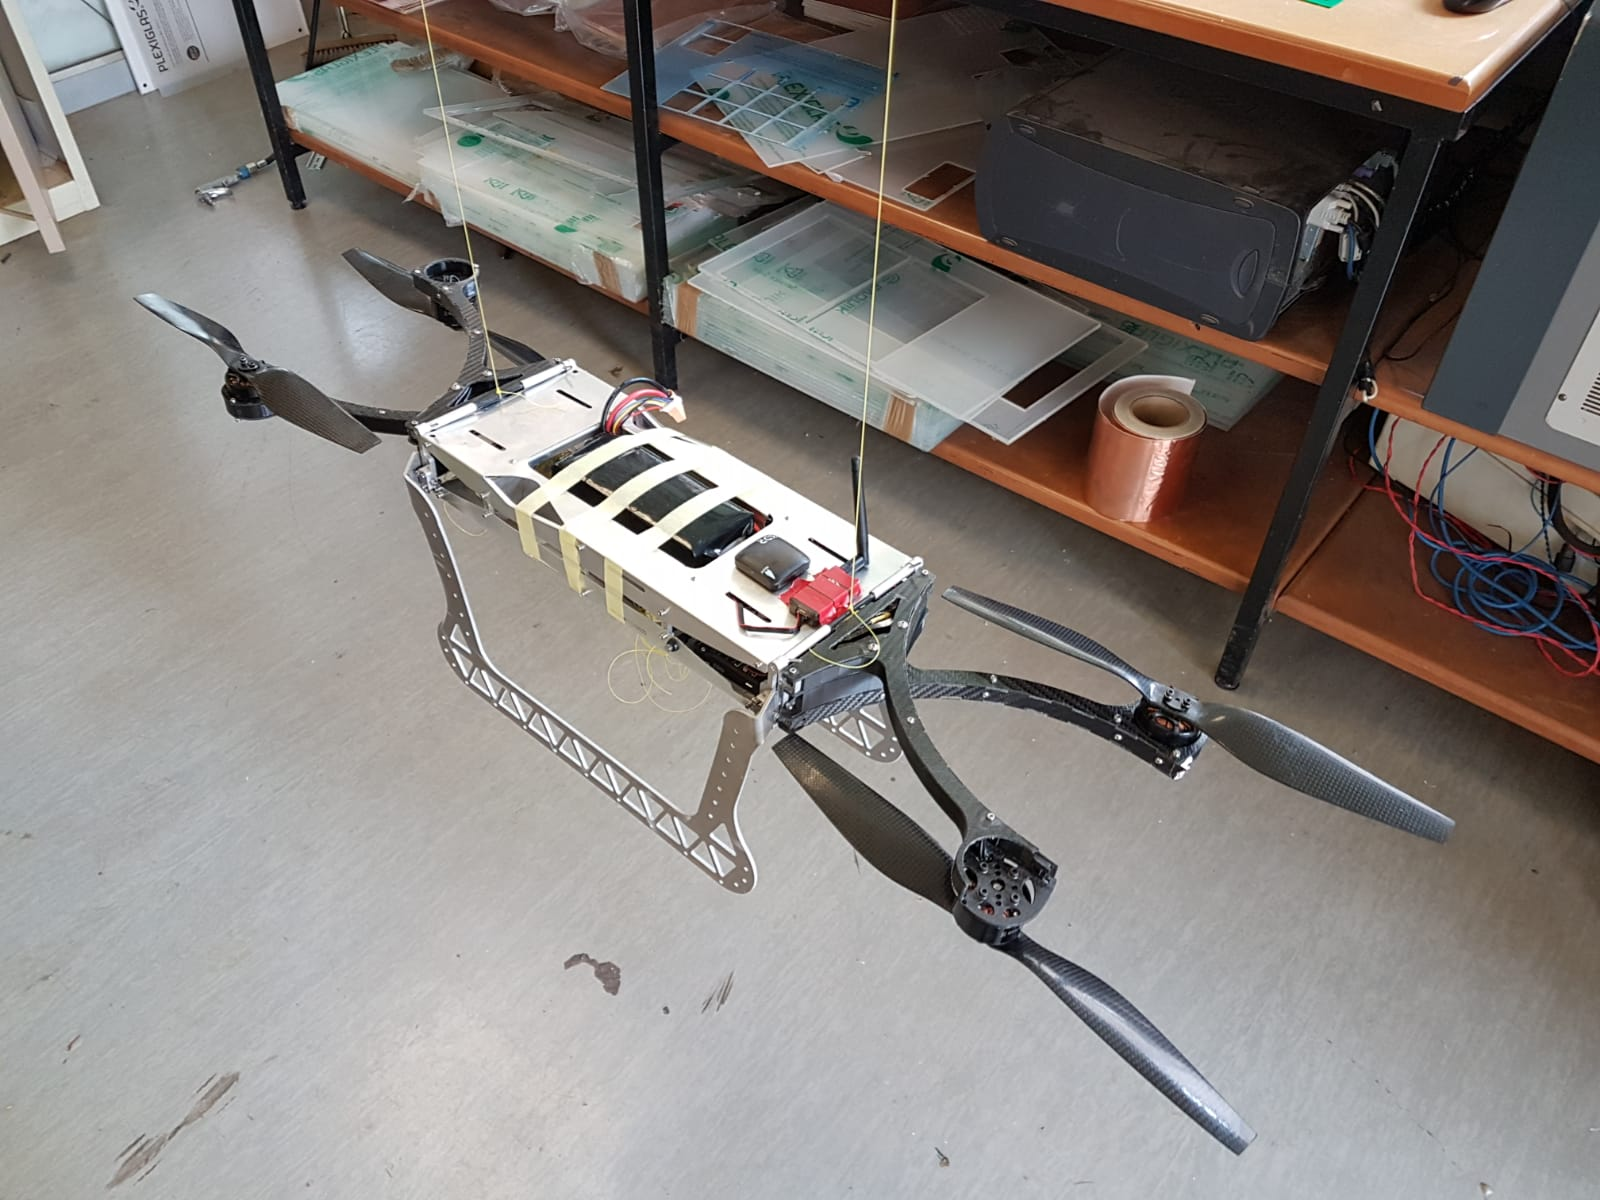
\includegraphics[height = 7.5cm]{Images/BifilarPendulum.jpeg}
		\caption{Bifilar Pendulum for Inertia Measurement}
		\label{IM_BifilarPendulum}
	\end{figure}
	
	Each axis was measured 10 times and the values were averaged out to obtain the final values represented in Table \ref{tab:MomentOfInertia}. To give a representation of measurement variance, the standard deviation is provided along side.
	
	\begin{table}[H]
		\centering
		\begin{tabular}{l | c | c | c |}
			Parameter & Averaged Measured Value & Standard Deviation\\
			\hline\hline
			$I_{xx}$ & 0.025027578 & 0.001063842\\
			$I_{yy}$ & 0.169260024 & 0.000142928\\
			$I_{zz}$ & 0.170196714 & 0.000527406\\
		\end{tabular}
		\label{tab:MomentOfInertia}
		\caption{Measured Moments of Inertia}
	\end{table}
	
	\subsection{Thrust and Moment Profiles}
	In order to correctly validate the thrust characteristics of the drone, each motor rotor pair needed to be evaluated. Each pair was marked and coupled to a load cell. The ESCs were configured to send varying PWMs to the motors. The commands sent to the ESCs and the measured thrust values are plotted together in Figure \ref{IM_ThrustProfiles}. Table \ref{tab:ThrustProfiles} gives the exact maximum and minimum values of each rotor motor pair. 
	
	\begin{figure}[H]
		\centering
		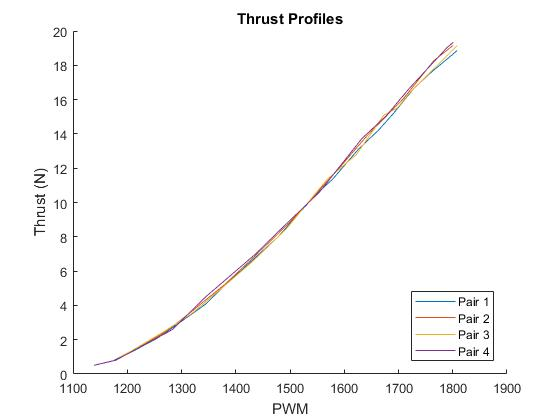
\includegraphics[height = 10cm]{../Design/Mechanical/ThrustProfiles/thrustprofiles.jpg}
		\caption{Thrust Ranges for Motor Rotor Pairs}
		\label{IM_ThrustProfiles}
	\end{figure}
	
	\begin{table}[H]
		\centering
		\begin{tabular}{l | c | c | c |}
			Pair & Max Thrust & Min Thrust\\
			\hline\hline
			$1$ & 18.8558 & 0.7852\\
			$2$ & 19.1489 & 1.1889\\
			$3$ & 19.1434 & 0.9511\\
			$4$ & 19.3369 & 0.5087\\
		\end{tabular}
		\caption{Measured Moments of Inertia}
		\label{tab:ThrustProfiles}
	\end{table}
	
	The motor lag constant for a similar sized craft and rotors was investigated in \cite{Moller2015} and found to be 0.125s. Each rotor is also subject to high frequency noise caused by undesired vibrations. The high frequency noise is modelled as a bandwidth limited white noise applied to each motor separately. 
	
	\subsection{Drag Coefficients}
	The drag coefficients chosen are that typically expected for a flat plate with an effective frontal area, as that seen in the fuselage of the craft. A $C_D$ of $1$ is chosen.
	
	The surface area of the drone was calculated by taking physical measurements of the drone and calculating the surface area from the measurements. Table \ref{tab:DragCoeff} records the calculated surface areas to be used in the calculation of each drag component. The last value in the table is the centre of gravity (COG) which was calculated to be located at the centre of the X and Y axis indicating symmetry along those axes, with a $3.5$\,cm offset in the Z-Axis. The centre of pressure (COP) is assumed as the centre of the craft, creating the required offset for the drag moments described in \ref{SSSECT_Drag}.
	
	\begin{table}[H]
		\centering
		\begin{tabular}{l | c |}
			Parameter & Value\\
			\hline\hline
			$A_x$ & 0.0354\\
			$A_y$ & 0.0693\\
			$A_z$ & 0.4\\
			$C_D$ & 1\\
			$COG$ & [0 0 0.035]\\
			$COP$ & [0 0 0]\\
		\end{tabular}
		\caption{Drag Coefficients}
		\label{tab:DragCoeff}
	\end{table}
	 
	\subsection{Sensor Constants}
	Investigation into the sensors used by the PixHawk, the proposed flight controller module, gives an indication of the sensor accuracy, resolution, noise and speed the drone measurements will be subject to.
	
	The PixHawk uses a combination of gyroscopes, accelerometers and magnetometers. The sensors used for the characterisation are the 6 DOF BMI055 which contains a 3-Axis accelerometer and a gyroscope along with the IST8310, 3-Axis magnetometer. Table \ref{tab:SensorCoeff} lists the extracted data.
	
	\begin{table}[H]
		\centering
		\begin{tabular}{l | c | c | c | c |}
			Sensor & Offset & Resolution & Noise & Maximum Bandwidth\\
			\hline\hline
			Accelerometer & $\pm70$\,mg & $0.98$\,mg & $150$\,$\mu$g/$\sqrt{Hz}$ & $1000$\,HZ\\
			Gyroscope & $\pm1$\,\textdegree/s & $0.1$\,\textdegree/s & $0.014$\,\textdegree/s/$\sqrt{Hz}$ & $1000$\,HZ\\
			Magnetometer & $\pm0.3$\,$\mu$T & $0.3$\,$\mu$T/LSB & NA & $200$\,Hz\\
		\end{tabular}
		\caption{IMU Sensor Coefficients}
		\label{tab:SensorCoeff}
	\end{table}
	
	For location and velocity measurements the GPS sensor used is the Neo-M8N developed by UBlox. Table \ref{tab:GPSCoeff} lists the relevant information obtained from the sensor datasheet.
	
	\begin{table}[H]
		\centering
		\begin{tabular}{l | c | c |}
			Sensor & Accuracy & Maximum Bandwidth\\
			\hline\hline
			Position & $2.5$\,m & $10$\,Hz\\
			Velocity & $0.05$\,m/s & $10$\,Hz\\
		\end{tabular}
		\caption{GPS Coefficients}
		\label{tab:GPSCoeff}
	\end{table}
	
	From the information gathered the sensors can now be modelled accordingly in Simulink. The IMU is modelled using the 3-Axis accelerometer block and the 3-axis gyroscope block in Simulink. The noise is set by using the above documented noise ratios. The GPS model utilises the Band-Limited White Noise Block in Simulink to create appropriate sensor noise. 

	\subsection{Wind Model}
	The wind model is broken into two portions, a constant wind and a more erratic, unpredictable wind both of which flow in the NED frame. The constant wind is defined as a configurable constant in the North East Down frame. The gust component is modelled as shown in Figure \ref{IM_WindModel}. The band limited white noise block is passed through a first order low pass filter to create a more realistic dynamic wind. The gain of the filter can be adjusted to observe effects of larger wind gusts on the craft.
	
	\begin{figure}[H]
		\centering
		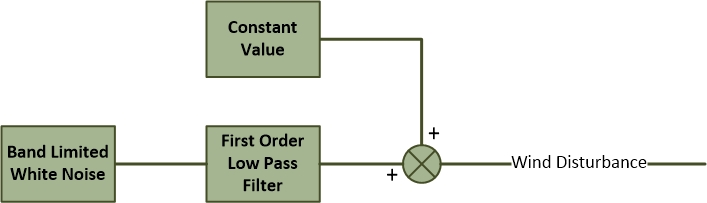
\includegraphics[height = 4cm]{../References/Diagrams/WindModel.jpg}     
		\caption{Wind Model}
		\label{IM_WindModel}
	\end{figure}
	
	The direction is commanded in the NED frame and rotated to apply the applicable forces to the body frame. The direction is modelled with a constant offset and varied by adding a small random number, smoothed by a low pass filter to create a more realistic wind direction variance.
			
\section{Simulation Configuration}\label{SECT_Nonlinear}
This section describes the process of creating the non linear simulation of the aircraft. The drone was modelled in Simulink using a combination of blocks included in the aerospace and control toolboxes, as well as a set of custom blocks. The model is required to successfully predict the position of the craft after being subjected to forces and moments. Using the dynamic flight model created above the bodies linear and rotational accelerations can be calculated by inputting forces and moments into the system. These accelerations can be subsequently integrated to achieve rates and positions. No model is 100\% accurate, however the information recorded in this chapter, when included, should create a solid estimation of the real world craft dynamics.

	\subsection{Motor Mixer}		
	The motor mixer is an important part of the control software running on the onboard computer and thus should be accurately modelled. This portion of code commands the ESCs of the drone to create the desired moments and forces. Section \ref{SSECT_RotorForcesMoments} explains how the rotors have control of four virtual actuators, these are $\delta_Z$, $\delta_{\theta}$, $\delta_{\psi}$ and $\delta_{\phi}$. The motor mixer is responsible for converting these desired moments and forces into actual values of thrust for each rotor.
	
	As Figure \ref{IM_MotorMixer} describes, each motor thrust value is made up of a summation of four thrust values,  $T_Z$, $T_{\theta}$, $T_{\psi}$ and $T_{\phi}$. Each value describes the rotor's contribution to the generation of that specific virtual actuator.
	 
	\begin{figure}[H]
		\centering
		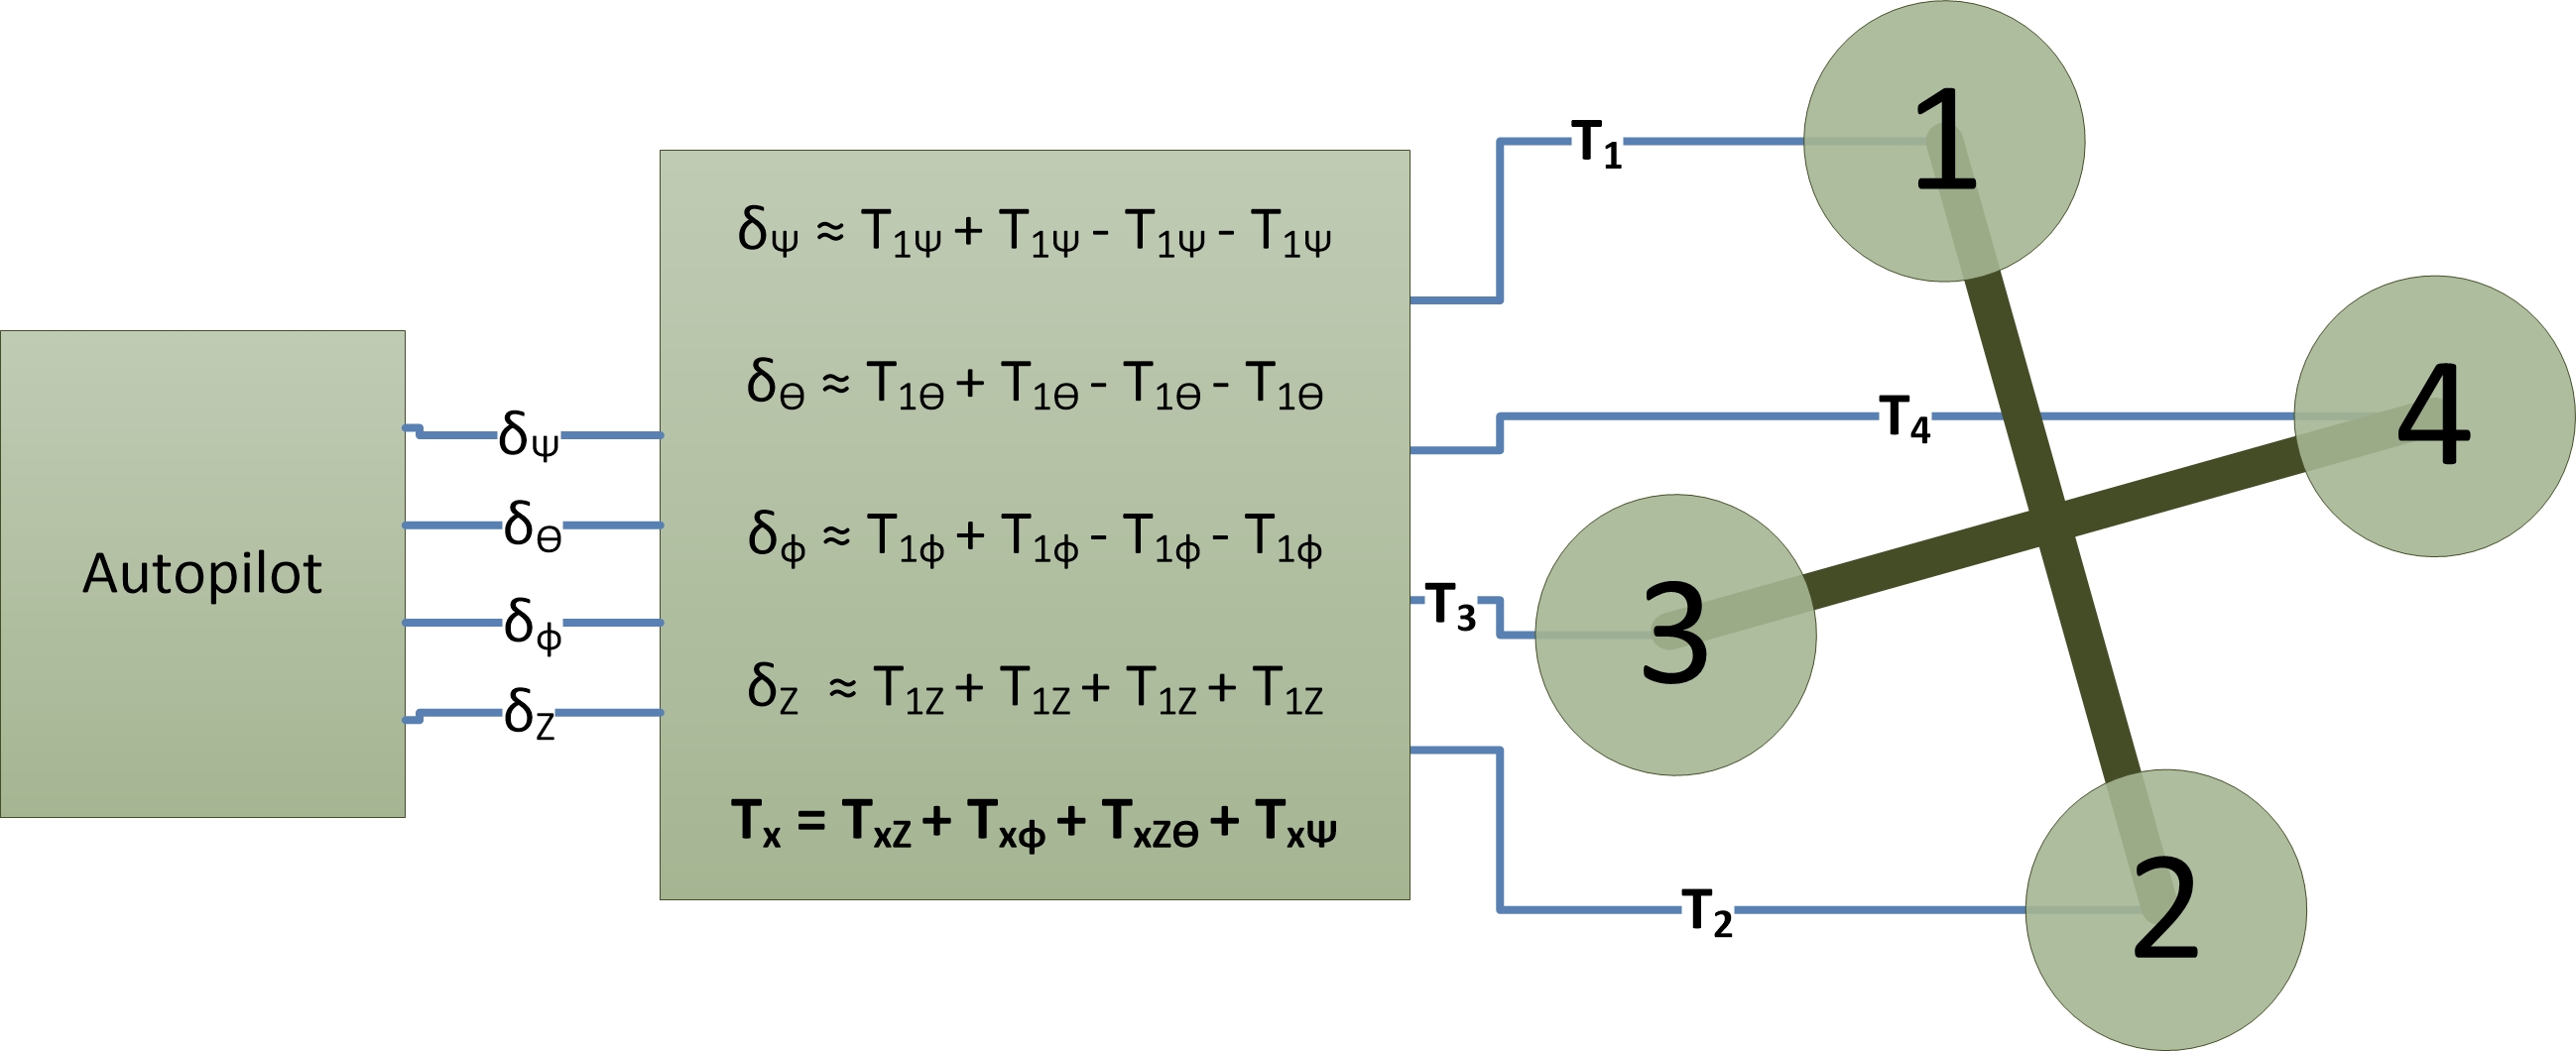
\includegraphics[height = 5cm]{../References/Diagrams/MotorMixer.jpg}
		\caption{Motor Mixer}
		\label{IM_MotorMixer}
	\end{figure}
	
	The motor mixer mathematics is based on the contribution provided by each rotor's thrust to the relevant virtual actuator. Assuming that each rotor only contributes a Z-Force it can be said that each rotor's thrust contributes 100\% of it's power to the virtual actuator $\delta_{Z}$. The roll and pitch virtual actuators are moment contributions and are calculated by evaluating the distance off the centre of gravity. Using the rotor arm length ($l$) and the angle ($\alpha$) a simple trigonometric relationship dictates the roll and pitch contributions. Finally the yaw contribution is calculated by taking into consideration the drag created by each rotor as it generates thrust. This relationship includes the lift to drag ratio ($R_{LD}$) of each rotor and the effective chord length ($r_D$) where the drag force is applied. Using all of these relationships the motor mixer's contribution matrix can be created and is shown in \eqref{EQ_MotorMixerMatrix}. The signs in the matrix are dictated by the body frame notation of positive directions and the placement of the rotors. The yaw contributions are dependant on the rotation direction of the rotors.

	\begin{equation}
	\label{EQ_MotorMixerMatrix}
	Contribution Matrix = 
	\begin{bmatrix}
	-1 & -1 & -1 & -1 \\
	l\sin\alpha & -l\sin\alpha & l\sin\alpha & -l\sin\alpha\\
	-l\cos\alpha & l\cos\alpha & l\cos\alpha & -l\cos\alpha \\
	-\dfrac{r_D}{R_{LD}} & -\dfrac{r_D}{R_{LD}} & \dfrac{r_D}{R_{LD}} & \dfrac{r_D}{R_{LD}} \\
	\end{bmatrix}
	\end{equation}
	
	The values for thrust can subsequently be calculated by multiplying the desired forces and moments by the inverse of the contribution matrix.


		
\chapter{Controller Design}
	 This chapter follows the stages of designing a controller for a quadrotor and begins by discussing the overall strategy. An analysis of existing rotorcraft control systems has been done in Section \ref{SECT_ControlReview}. The system must be able to follow waypoint commands, containing a position reference in the North, East and Down frame. As well as align with a desired heading, this reference will be in the form of a Euler angle. The rest of the design goals are discussed before the controller design is begun.
	 
	 \section{Design Goals}
	 
	 
	 \section{Flight Control Strategy}
	 Figure \ref{IM_ControlStrategy} represents the high level control strategy for this project and indicates their sampling frequencies. This discussion will break the system into three main components: an altitude controller, a horizontal flight controller and a heading controller.	
	 
	 The altitude controller starts by getting a position reference in the earth frame. This reference is fed through a PI controller to create a desired climb rate. The climb rate reference is converted into the body frame and is then controlled using a P controller to produce a body acceleration reference. The heave controller can only produce a force perpendicular to the rotor, thus this component is taken and fed through an additional PI heave controller. The output of this inner heave controller would be the virtual actuator $\delta_Z$.
	 
	 The horizontal controller gets both a North and an East position reference and uses PI controllers to create velocity setpoints in the earth frame. These setpoints are converted to the body frame where the linear velocity controller works and outputs acceleration references in the body frame. Using the body acceleration references, roll and pitch rate setpoints can be created using a tilt angle controller. These rate set points are fed into the inner rate loop controller which output the virtual actuators $\delta_\phi$ and $\delta_\theta$.
	 
	 Lastly the heading controller is discussed. Correct design of the tilt angle controller will decouple the vehicle's horizontal controller from a dependency on the heading of the craft. This allows seamless implementation of a heading controller. The heading controller is broken down into two parts: a yaw angle and a yaw rate controller. The output of this controller is the virtual actuator $\delta_\psi$.
	 
	 \begin{figure}[H]
	 	\centering
	 	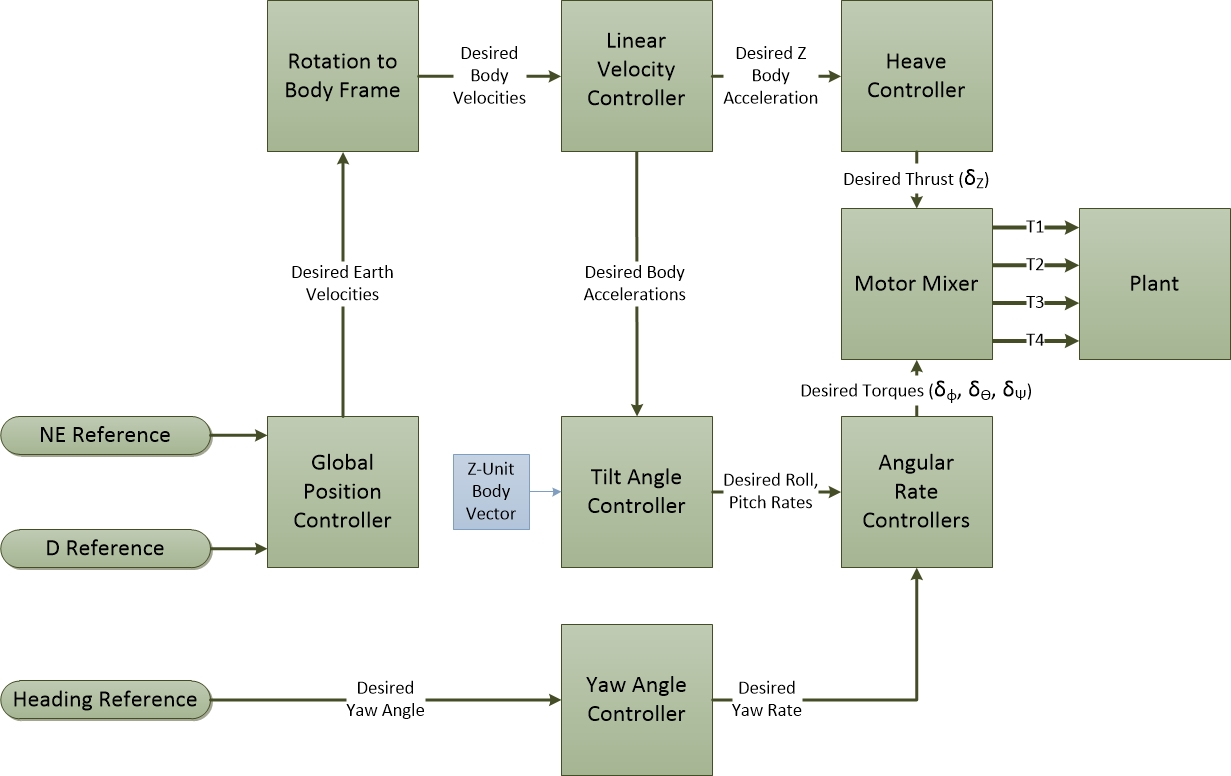
\includegraphics[height = 10cm]{../References/Diagrams/HighLevel.jpg}
	 	\caption{High Level Control Strategy}
	 	\label{IM_ControlStrategy}
	 \end{figure}
	 
	 \section{Altitude Controller}
	 This section discusses the implementation of the altitude controller. The overall altitude controller is structured as a set of cascaded control loops, with the most inner loop controlling the aircraft's acceleration and the most outer loop controlling the desired altitude in the earth frame. In order to control the altitude of a craft, an analysis of the system's heave dynamics must first be performed. Once a mathematical model has been created, an inner PI heave controller is applied to follow a desired vertical acceleration reference. The climb rate P controller is responsible for generating these acceleration references and is fed a desired linear vertical velocity reference by the altitude hold P controller. 
	 
	 \subsection{Heave Dynamics}
	 Using Newton mechanics at near hover conditions for the aircraft, the heave dynamics can be derived and are shown in \eqref{EQ_HeaveNewton}. Where $\dot{W}$ is the current acceleration of the craft in the Z-Axis and $m$ is the vehicles's mass. $Z$ is defined as the current instantaneous force being produced by the rotors.
	 
	 \begin{equation}
	 \label{EQ_HeaveNewton}
	 \dot{W} = \dfrac{Z}{m}
	 \end{equation}
	 
	 The state variable of the system is chosen as $Z$ with the output of this plant being $\dot{W}$. Using the transfer function for motor-rotor lag dynamics seen in \eqref{EQ_MotorDelay} and the dynamics seen in \eqref{EQ_HeaveNewton}, the state space equation for the system can be derived and is shown in \eqref{EQ_HeaveStateSpace1} and \eqref{EQ_HeaveStateSpace2}. 
	 
	 \begin{eqnarray}
	 [\dot{Z}] &=& - [\dfrac{1}{\tau}] \ [Z] + [\dfrac{1}{\tau}] [\delta_Z]\label{EQ_HeaveStateSpace1}\\\label{EQ_HeaveStateSpace11}
	 [\dot{W}] &=& - [\dfrac{1}{m}] \ [Z]\label{EQ_HeaveStateSpace2}
	 \end{eqnarray}
	 
	 Subsequently the transfer function can be calculated and the result is shown in \eqref{EQ_HeaveTF}. The negative gain of the transfer function must be noted and is caused by the direction of the defined axes, with the rotors producing a negative Z-Axis force.
	 
	 \begin{equation}
	 G(s)_{heave} = \frac{\frac{-1}{m \times \tau}}{s + \frac{1}{\tau}}\label{EQ_HeaveTF}
	 \end{equation}
	 
	 The rotor motor lag produces the pole at $\dfrac{-1}{\tau} = -8$ and indicates the maximum response capabilities and timing constant of the rotor system.
	 
	 \subsection{Heave Controller}
	 The heave controller is responsible for commanding the $\delta_Z$ virtual actuator to achieve a desired Z-Axis acceleration in the body frame. The model derived above can be shown to produce a large steady state error. A PI architecture was initially chosen as shown in Figure \ref{IM_HeaveController}. 
	 
	 The integrator is used to remove the steady state error, while the most left limiter shown in Figure \ref{IM_HeaveController} was added to stop integrator wind up and is not considered during the linear controller design. The proportional gain is used to move the closed loop poles and achieve the desired bandwidth. The dynamic response of the system can be investigated using the root locus and bode plots shown in Figure \ref{IM_HeaveControlRoot} and \ref{IM_HeaveControlBode}. 
	 
	 \begin{figure}[H]
	 	\centering
	 	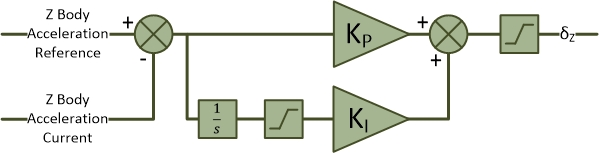
\includegraphics[height = 3.5cm]{../References/Diagrams/HeaveController.jpg}
	 	\caption{Heave Controller -  Control Diagram}
	 	\label{IM_HeaveController}
	 \end{figure}
	 
	 Figure \ref{IM_HeaveControlRoot} shows the root locus of the system with the PI controller included. The controller introduces a new pole at the origin. To maintain a first order response, the zero is placed close to the plant pole. This placement will attenuate the open loop, plant pole's response. Finally the gain is varied until the closed loop responses are closely aligned with the naturally occurring open loop pole. The final closed loop poles are a set of complex poles and are located at $-7.55 \pm 3.64 i$. The frequency response can be evaluated using the bode plot in Figure \ref{IM_HeaveControlBode}. 
	 
	 \begin{figure}[H]
	 	\centering
	 	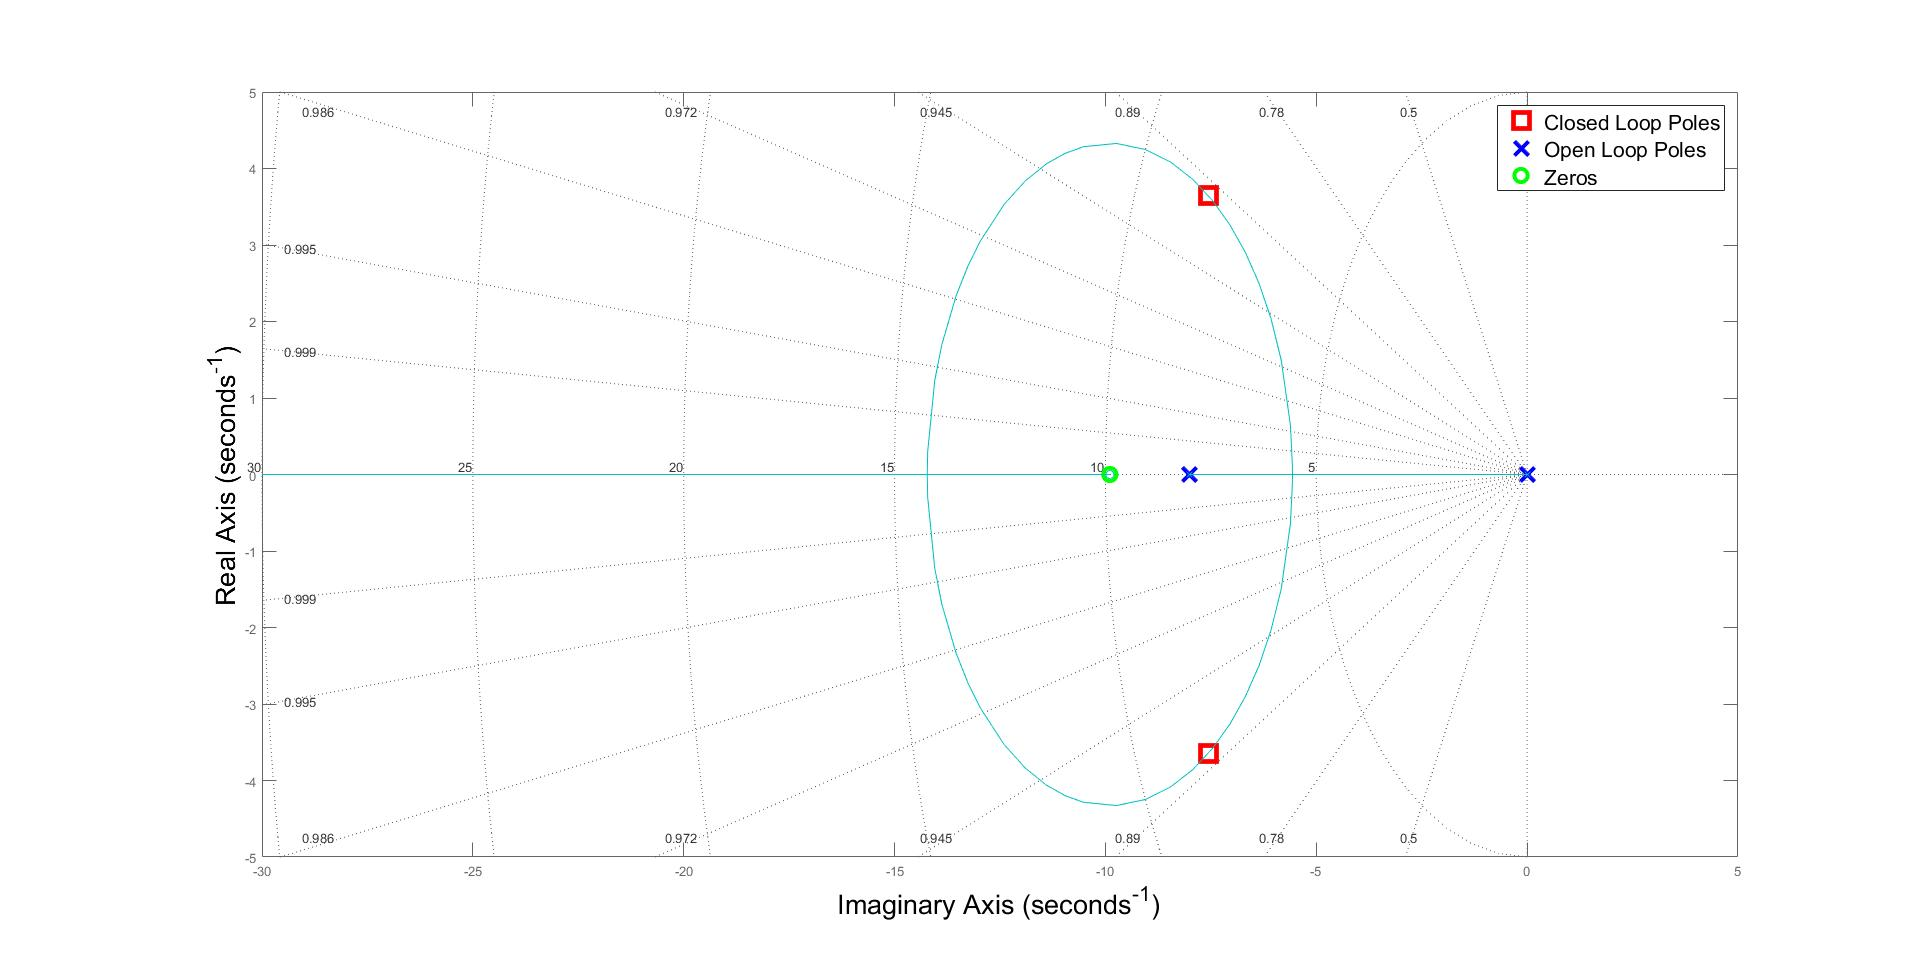
\includegraphics[height = 8cm]{../Design/Matlab/Controllers/heave_root.jpg}
	 	\caption{Heave Controller -  Root Locus}
	 	\label{IM_HeaveControlRoot}
	 \end{figure}
	 
	 The final cross over frequency is shown on the bode plot for the heave controller in Figure \ref{IM_HeaveControlBode}. The gain plot shows the controller adjust the crossover frequency to $7.99 Rad/s$ which is close to the limit of the system. The controller also increases the phase of the system and has a final phase margin of $83.96$\textdegree. The resultant control law is shown in \eqref{EQ_HeaveController}.
	 
	 \begin{equation}
	 \label{EQ_HeaveController}
	 C(s)_{heave} = \frac{2.9782 (s + 9.985)}{s}
	 \end{equation}		
	 
	 \begin{figure}[H]
	 	\centering
	 	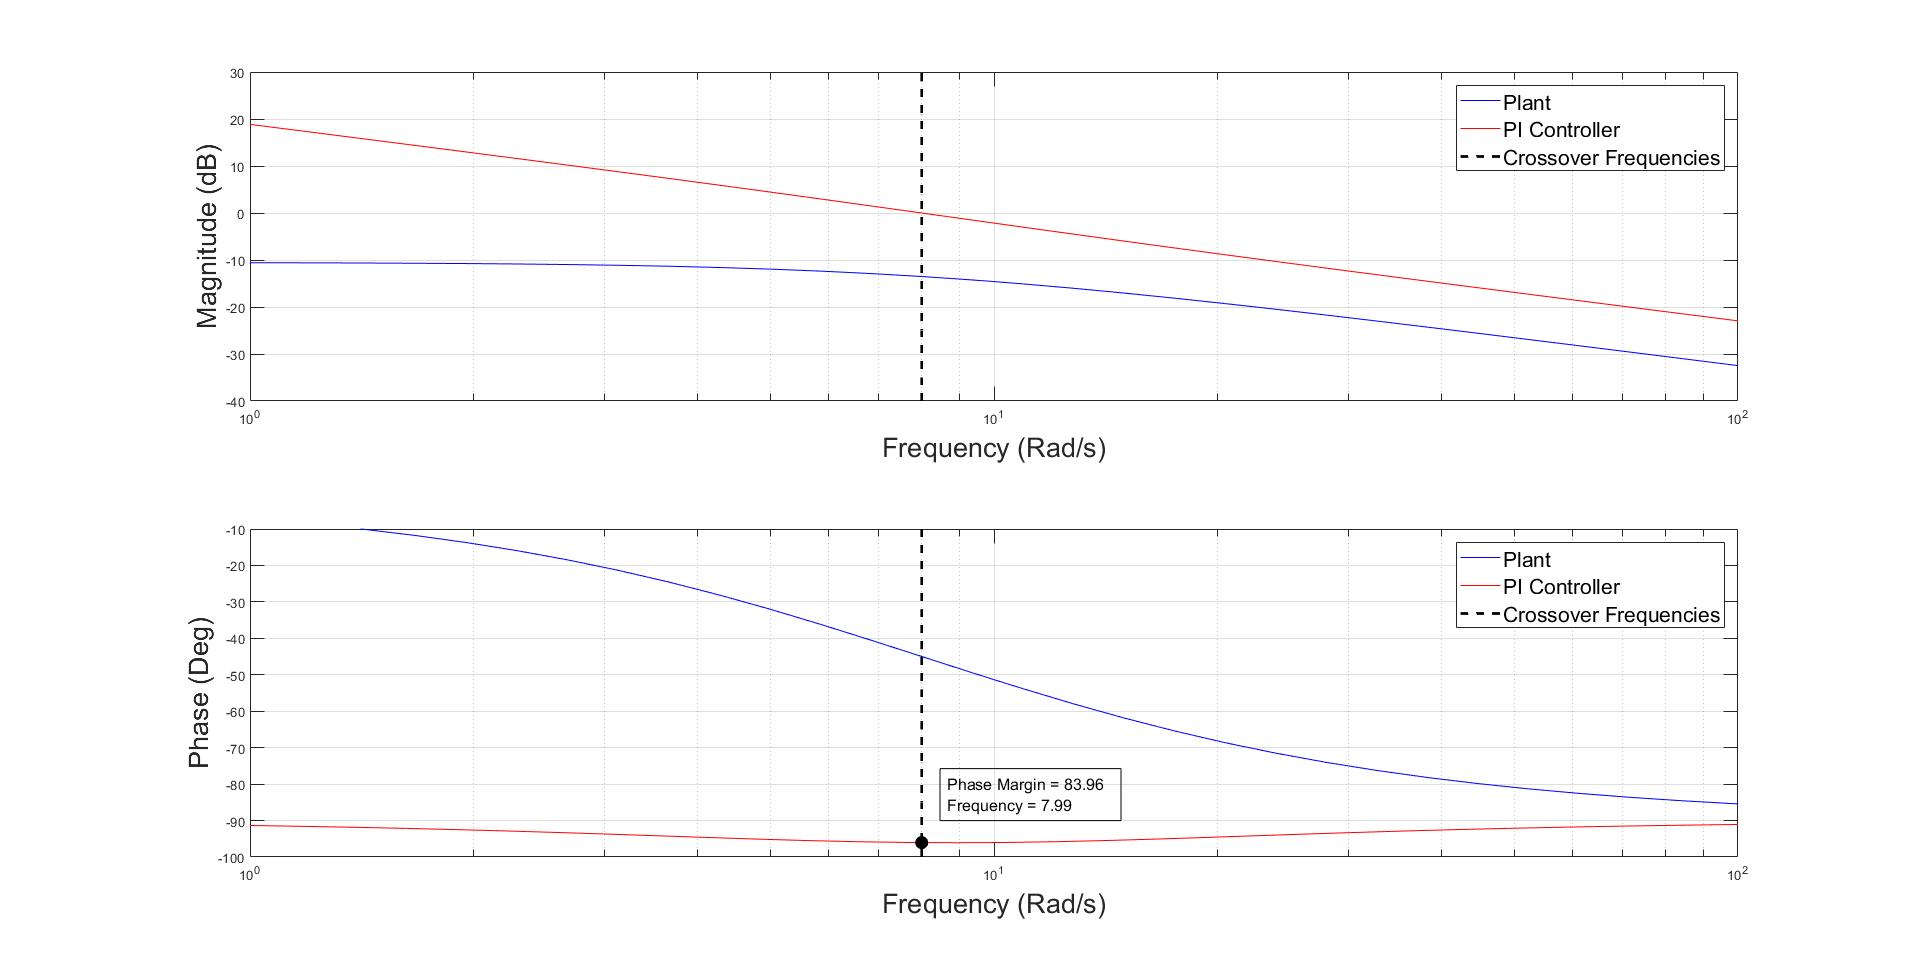
\includegraphics[height = 8cm]{../Design/Matlab/Controllers/heave_bode.jpg}
	 	\caption{Heave Controller -  Bode Plots}
	 	\label{IM_HeaveControlBode}
	 \end{figure}
	 
	 An additional non linear element in the form of a limiter is brought into the system to limit the maximum and minimum thrust commands. The maximum limit is used to ensure the heave controller does not saturate the motors. This creates headroom for the angular rate controllers and disturbance rejection. The lower limit is used to ensure the vehicle always descends at a steady pace. The maximum thrust capabilities are displayed in table \ref{tab:ThrustProfiles}, summing these values produces a total maximum thrust of approximately $76N$ for the total rotor system. The final limits chosen are shown in Table \ref{tab:HeaveLimits}.
	 
	 \begin{table}[!]
	 	\centering
	 	\begin{tabular}{l | c | c |}
	 		Limit Name 				& Min & Max\\
	 		\hline\hline
	 		Integrator Wind Up 	   	& -1.5 	& 1.5 \\
	 		Thrust Command 		    & 10	& 55 \\
	 	\end{tabular}
	 	\caption{Heave Controller Limits}
	 	\label{tab:HeaveLimits}
	 \end{table}
	 
	 
	 
	 \subsubsection{Heave Controller Discussion}
	 Now that the system presents stable dynamic results in the frequency and Laplace domains, using the non-linear simulation, the time domain responses can be discussed in brief. The resultant step response, including the PI controller, is shown in Figure \ref{IM_HeaveStepDist}. To demonstrate the disturbance rejection capabilities of the design, a force of $10N$ is applied to the drone at $2.5s$.
	 
	 \begin{figure}[H]
	 	\centering
	 	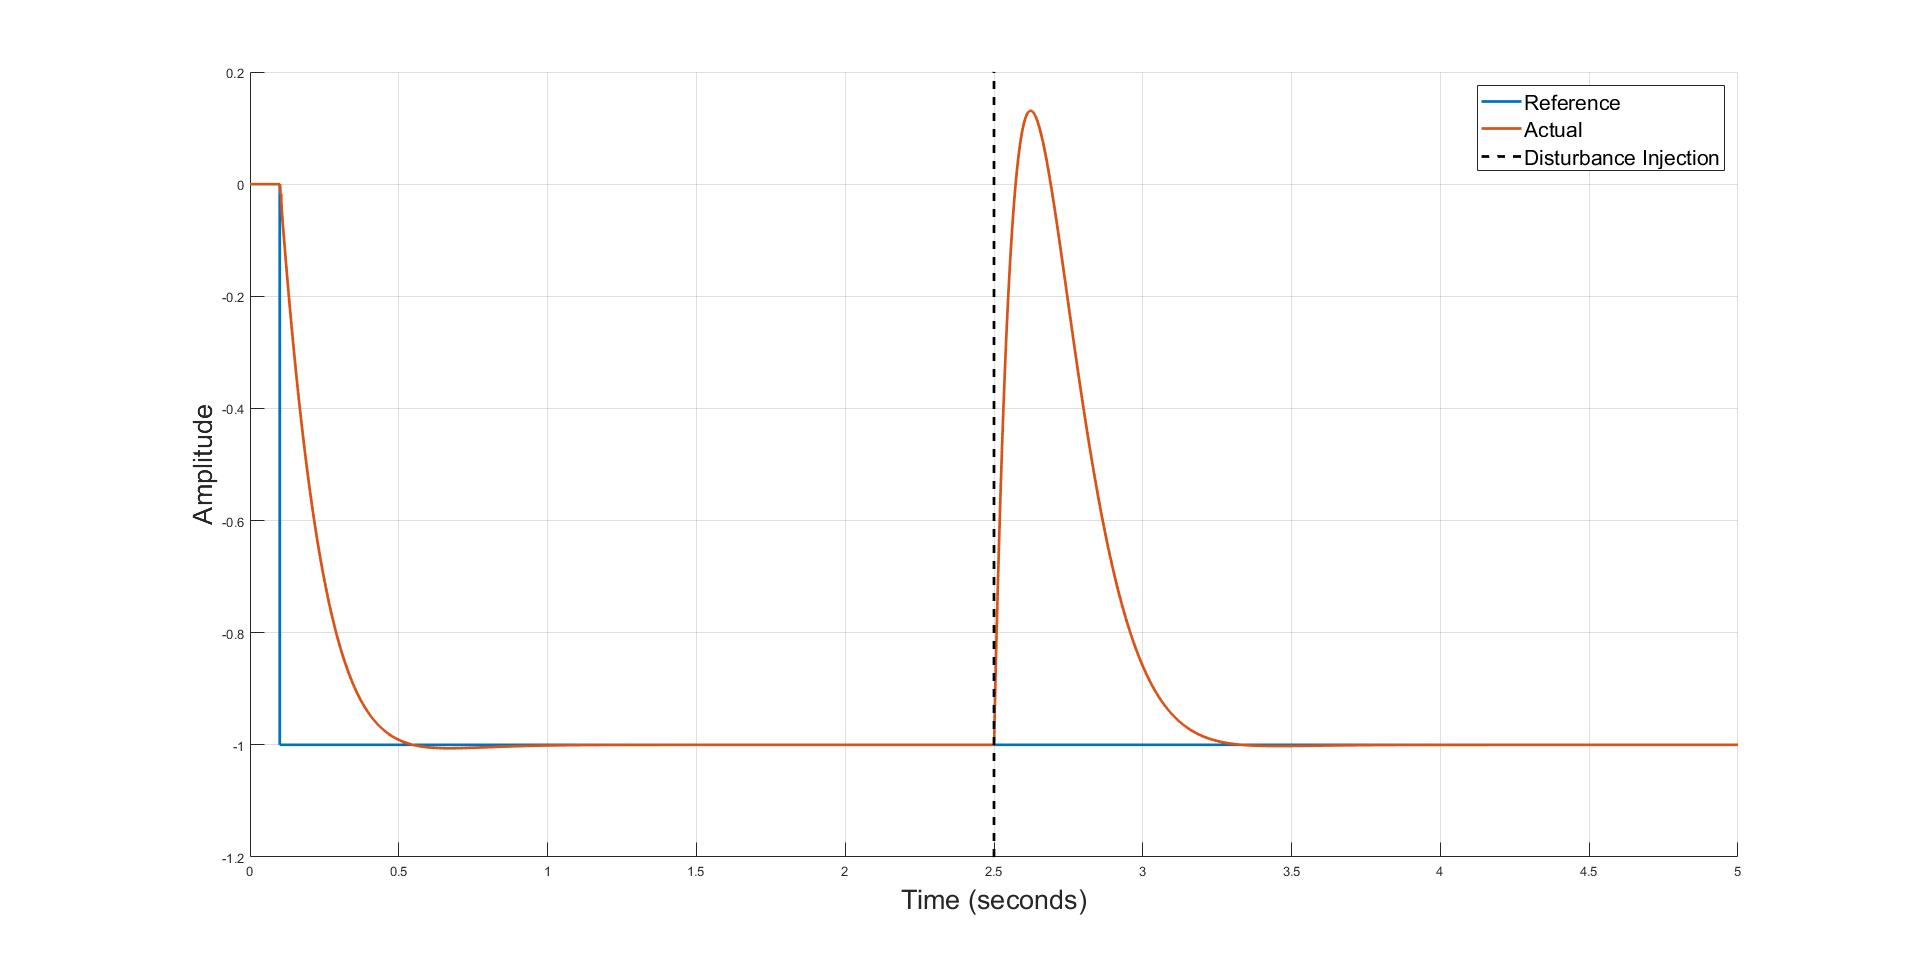
\includegraphics[height = 8cm]{../Design/Matlab/Controllers/heave_step.jpg}
	 	\caption{Heave Controller -  Step Response}
	 	\label{IM_HeaveStepDist}
	 \end{figure}
	 
	 The heave controller, as the most inner loop, limits the response for the rest of the altitude control system. The proposed design brings the heave loop response close to the limits of the plant, thus producing a similar (but slower) timing constant to that of the motor-rotor system. The system reaches and settles within 5\% of the reference by $0.313s$, is critically damped and presents negligible overshoot. The system also shows to be capable of tracking an acceleration setpoint with zero steady state error. As shown in Figure \ref{IM_HeaveStepDist} the system can also respond quickly to a large, sudden and constant disturbance.
	 
	 \subsection{Climb Rate Controller}
	 The climb rate controller is responsible for controlling the vertical velocity of the aircraft, in the earth frame. This introduces the need for rotating either the reference or the command into the body frame. The decision can be made by considering the frame in which the sensing information is provided. Most aircraft make use of some form of global positioning system and using differentiation can calculate speed. However, due to the application environment, this aircraft will most likely use a velocity measurement sensor relative to the body frame. The architecture for the climb rate controller is outlined in Figure \ref{IM_ClimbRateControlLoop}. 
	 
	 The speed of the climb rate controller is limited by the inner heave leave control loop, this becomes a limiting design criterion for the system.
	 
	 \begin{figure}[H]
	 	\centering
	 	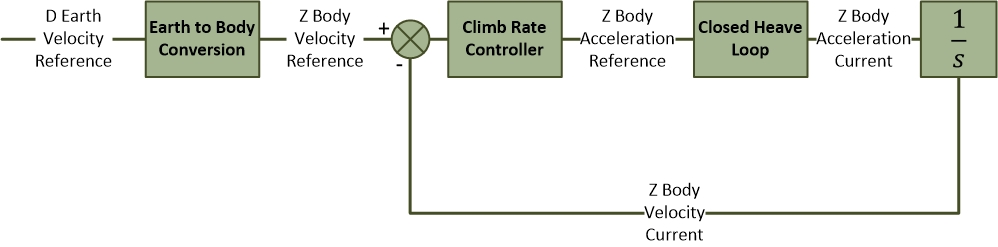
\includegraphics[height = 3.75cm]{../References/Diagrams/ClimbRateLoop.jpg}
	 	\caption{Climb Rate Controller Closed Loop}
	 	\label{IM_ClimbRateControlLoop}
	 \end{figure}
	 
	 At near hover conditions the plant can be linearised and the rotation can be excluded. Figure \ref{IM_ClimbRateController} shows the simplified climb rate controller architecture. The computational time required for rotating the references can be considered by ensuring the controller design provides a reasonable phase margin. The open loop poles of the climb rate system are located at the closed loop pole positions of the inner heave system, while the mathematical relationship between acceleration and velocity yields an additional open loop pole at the origin.
	 
	 \begin{figure}[H]
	 	\centering
	 	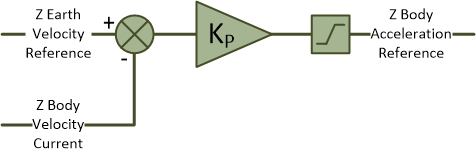
\includegraphics[height = 3.5cm]{../References/Diagrams/ClimbRateController.jpg}
	 	\caption{Climb Rate Controller}
	 	\label{IM_ClimbRateController}
	 \end{figure}		
	 
	 The free integrator in the plant ensures the system will track a step response with zero steady state error while the proportional gain is used to speed up the system and achieve the desired bandwidth.
	 The dynamic response of the system, including the controller, is evaluated using the root locus and bode plots shown in Figure \ref{IM_ClimbRateRoot} and \ref{IM_ClimbRateBode}.
	 
	 \begin{figure}[H]
	 	\centering
	 	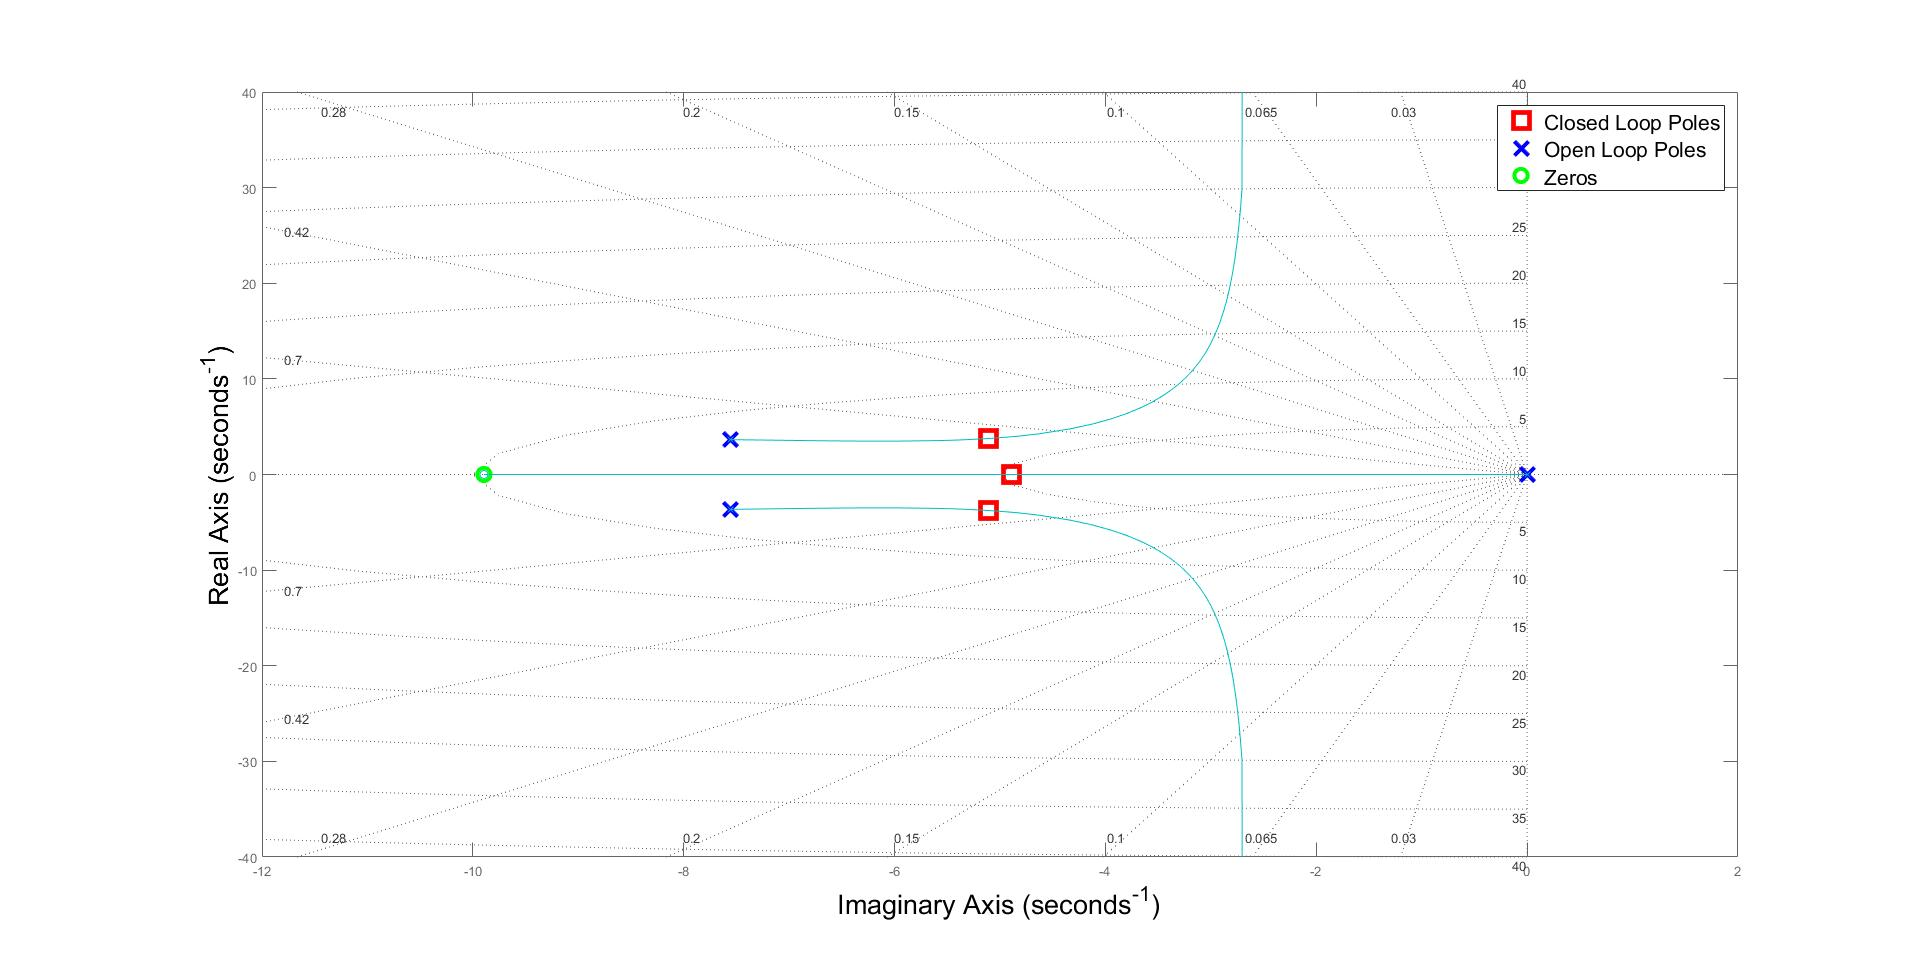
\includegraphics[height = 8cm]{../Design/Matlab/Controllers/climb_rate_root.jpg}
	 	\caption{Climb Rate Controller -  Root Locus}
	 	\label{IM_ClimbRateRoot}
	 \end{figure}
	 
	 Figure \ref{IM_ClimbRateRoot} shows the location of the three final closed loop poles. The complex pair is placed at $-5.11 \pm 3.76i$ and the integrator pole is located at $-4.89$ and is on the imaginary axis.
	 
	 \begin{figure}[H]
	 	\centering
	 	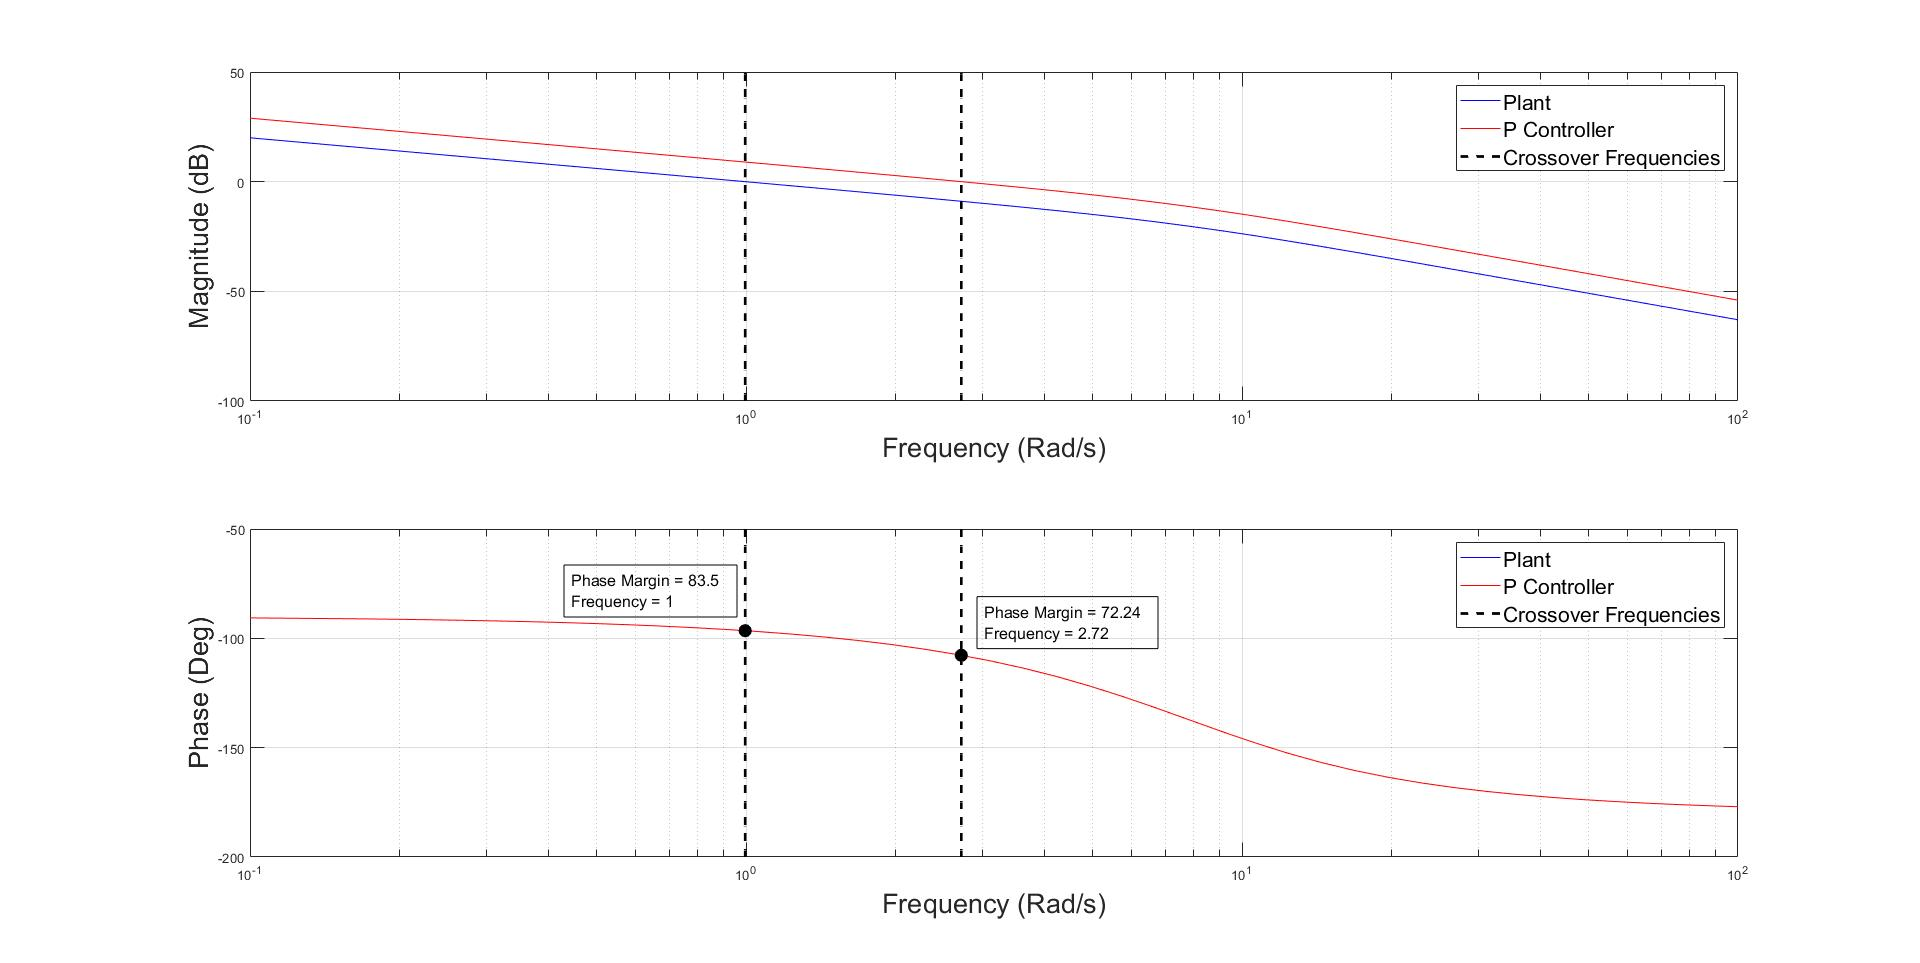
\includegraphics[height = 8cm]{../Design/Matlab/Controllers/climb_rate_bode.jpg}
	 	\caption{Climb Rate Controller - Open-Loop Bode Plots}
	 	\label{IM_ClimbRateBode}
	 \end{figure}
	 
	 The bode plot shown in \ref{IM_ClimbRateBode} shows zero change in phase due to the controller architecture. The gain however is increased and moves the crossover frequency to $2.72 Rad/s$. The ratio of inner and outer loop crossover frequencies is then $2.91$, providing enough bandwidth between the inner and outer loops. The phase margin can then be calculated to be $72$\textdegree. 
	 
	 As shown in Figure \ref{IM_ClimbRateController} there is a limiter applied to the acceleration commands. This limit is present due to the confined operational environment and ensures that the climb rate controller does not saturate the horizontal velocity controllers. The final limits are shown in Table \ref{tab:ClimbrateLimits}
	 
	 \begin{table}[!]
	 	\centering
	 	\begin{tabular}{l | c | c |}
	 		Limit Name 						& Min & Max\\
	 		\hline\hline
	 		Acceleration Command 		    & -5 & 5 \\
	 	\end{tabular}
	 	\caption{Climb Rate Controller Limits}
	 	\label{tab:ClimbrateLimits}
	 \end{table}
	 
	 \subsubsection{Climb Rate Controller Discussion}
	 The dynamic response shows sufficient phase margin to handle unmodelled timing delays. While the ratio between the inner controller ensures this controller will not be attenuated. The step response of the closed loop system is shown in Figure \ref{IM_ClimbRateStep}. The system has a $5$\% settling time of $0.747s$ and shows negligible overshoot. At $5s$ a disturbance of $10N$ is placed on the rotors and the system demonstrates the ability to continue tracking the desired setpoint with zero steady state error.
	 
	 \begin{figure}[H]
	 	\centering
	 	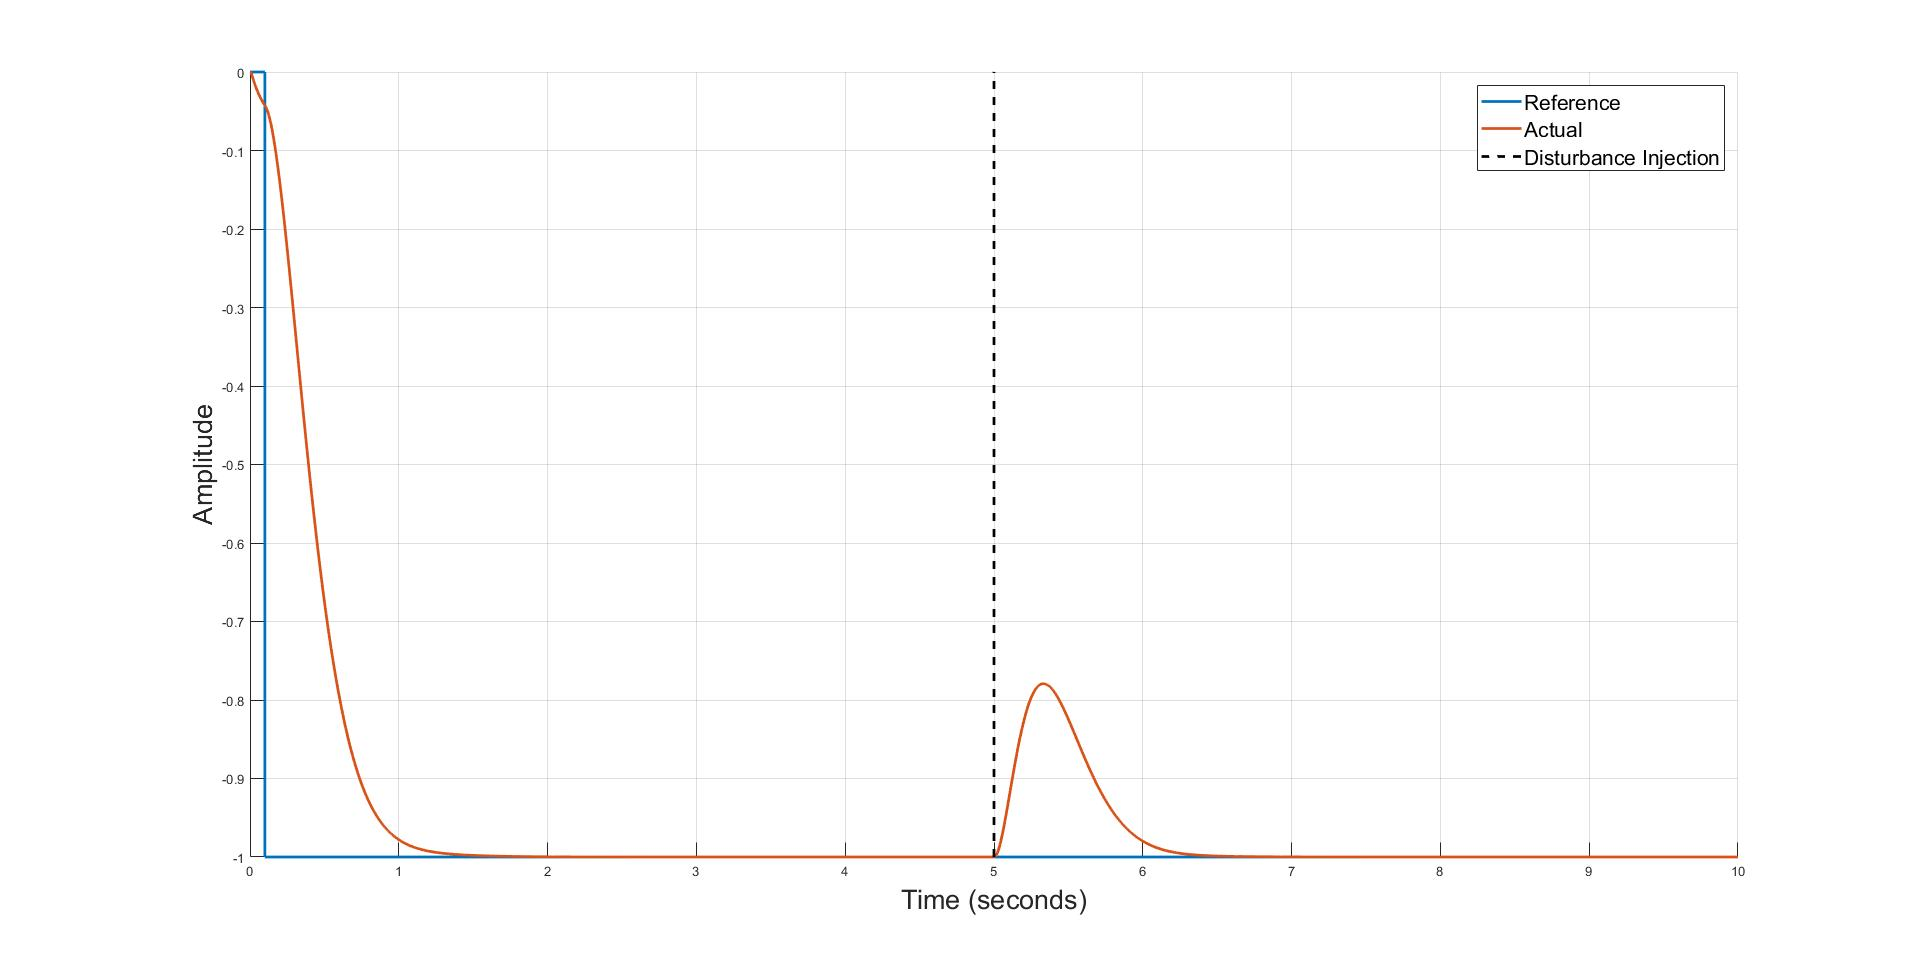
\includegraphics[height = 8cm]{../Design/Matlab/Controllers/climb_rate_step.jpg}
	 	\caption{Climb Rate Controller -  Step Response}
	 	\label{IM_ClimbRateStep}
	 \end{figure}
	 
	 \subsection{Altitude Hold Controller}
	 The final stage of the vertical control system is the altitude hold controller. This controller receives a desired altitude in the earth frame and outputs a reference velocity, also in the earth frame. The closed control loop block diagram is shown in Figure \ref{IM_AltHoldControlLoop}. This controller is limited by the response time of the inner loops and must be considered in the design.
	 
	 \begin{figure}[H]
	 	\centering
	 	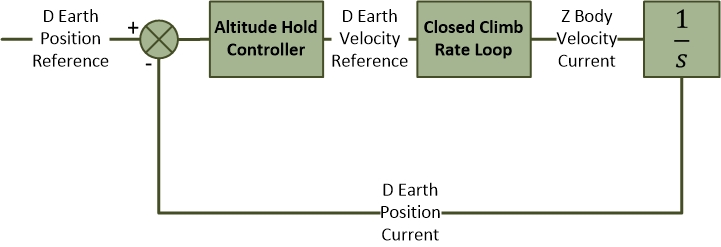
\includegraphics[height = 4cm]{../References/Diagrams/AltHoldLoop.jpg}
	 	\caption{Altitude Hold Controller Closed Loop}
	 	\label{IM_AltHoldControlLoop}
	 \end{figure}
	 
	 The chosen controller architecture is shown in Figure \ref{IM_AltHoldController}. The proportional gain is used to vary the bandwidth to be within the limits of the system. The faded integrator shown in Figure \ref{IM_AltHoldController} is not considered during linear analysis. The integrator shall be limited in such a way as to limit the interference of the proportional gain. The reason for including the integrator is to ensure the system can track measurement errors in velocity with zero steady state error and exhibit a first order response. A PID controller architecture was also considered and the analysis was done for both control laws.
	 
	 The system's dynamic response is analysed using the root locus shown in Figure \ref{IM_AltHoldRoot} and the bode plot shown in Figure \ref{IM_AltHoldBode}.
	 
	 \begin{figure}[H]
	 	\centering
	 	\includegraphics[height = 3.5cm]{../References/Diagrams/AltHoldController.jpg}
	 	\caption{Altitude Hold Controller}
	 	\label{IM_AltHoldController}
	 \end{figure}
	 
	 Figures \ref{IM_AltHoldRoot} and \ref{IM_AltHoldBode} evaluate a P controller against a PID controller. The P controller adds no new poles or zeros and the closed loop poles of the P controlled system are placed at $-5.52 \pm 3.23i$ and $-2.03 \pm 0.58i$. 
	 The PID controller adds an additional pole and two additional zeros into the system. The closed loop poles of the PID controlled system are located at $-6.64$, $-3.59 \pm 5.03i$ and $-0.64 \pm 0.47i$. The two new zeros are placed at $-0.57$ and $-2.06$.
	 
	 \begin{figure}[H]
	 	\centering
	 	\includegraphics[height = 8cm]{../Design/Matlab/Controllers/altitude_root.jpg}
	 	\caption{Altitude Hold Controller -  Root Locus}
	 	\label{IM_AltHoldRoot}
	 \end{figure}
	 
	 The bode plot shows the PID controller producing a final cross over frequency of $1.90Rad/s$, this response is too fast for the inner climb rate system and will need to be redesigned or discarded. The P controller exhibits a cross over frequency of $0.91Rad/s$, this produces a ratio of $3.03$ between the inner and outer loops and a phase margin of $71.5$\textdegree. The phase of the system using a P controller crosses the $180$\textdegree  $\ $mark at $4.81Rad/s$ and has a gain margin of $18.7dB$.
	 
	 \begin{figure}[H]
	 	\centering
	 	\includegraphics[height = 8cm]{../Design/Matlab/Controllers/altitude_bode.jpg}
	 	\caption{Altitude Hold Controller -  Bode Plots}
	 	\label{IM_AltHoldBode}
	 \end{figure}
	 
	 To finalise the design, the two limiters are discussed. The first limiter is used to limit the effect of the integrator on the system as well as stop integrator wind up. The second limiter is used to limit the climb rate commands sent to the inner controllers. Both sets of limits are shown in Table \ref{tab:AltitudeControllerLimits}
	 
	 \begin{table}[!]
	 	\centering
	 	\begin{tabular}{l | c | c |}
	 		Limit Name 						& Min & Max\\
	 		\hline\hline
	 		Integrator Wind Up 				& -0.09 & 0.09 \\
	 		Climb Rate Command 		    	& -5 & 5 \\
	 	\end{tabular}
	 	\caption{Altitude Hold Controller Limits}
	 	\label{tab:AltitudeControllerLimits}
	 \end{table}
	 
	 \subsubsection{Altitude Hold Controller Discussion}
	 Although both the P and PID controllers exhibit stable dynamic responses, the PID controller exhibited too fast a response and will be effected by the inner controllers. The system including only a P controller exhibits a step response as shown in Figure \ref{IM_AltHoldStep}, a disturbance of $10N$ is applied to the rotors at $10s$. The system has a $5\%$ settling time of $2.29s$ and tracks the set point with zero steady state error. The system handles the disturbance with a maximum overshoot of $0.01m$ and is critically damped.
	 
	 \begin{figure}[H]
	 	\centering
	 	\includegraphics[height = 8cm]{../Design/Matlab/Controllers/altitude_step_p_no_dist.jpg}
	 	\caption{Altitude Hold P Controller -  Step response}
	 	\label{IM_AltHoldStep}
	 \end{figure}
	 
	 However, if a measurement disturbance is present in the inner loops, this system will not track a setpoint with zero steady state error. To demonstrate this a constant offset of $0.05m/s$ is placed on the Z-Axis velocity measurement, Figure \ref{IM_AltHoldPDistStep} shows the current system cannot account for this disturbance. As shown in \ref{IM_AltHoldController}, a limited gain integrator is introduced into the system to help the system track steady state error. 
	 
	 \begin{figure}[H]
	 	\centering
	 	\includegraphics[height = 8cm]{../Design/Matlab/Controllers/altitude_step_p_dist.jpg}
	 	\caption{Altitude Hold P Controller -  Step response with inner loop measurement offset}
	 	\label{IM_AltHoldPDistStep}
	 \end{figure}
	 
	 The new controller must be limited in such a way as to exhibit a similar transient response as the existing P controller. Figure \ref{IM_AltHoldPIDistStep} shows the step response of the new system both with and without the $0.05m/s$ offset in the velocity measurement. As shown, the P controller including a limited I component introduces more overshoot into the system. The limits are designed to ensure the new controller introduces less than 10\% overshoot into the system. 
	 
	 \begin{figure}[H]
	 	\centering
	 	\includegraphics[height = 8cm]{../Design/Matlab/Controllers/altitude_step_pi.jpg}
	 	\caption{Altitude Hold P with Limited I Controller -  Step Responses}
	 	\label{IM_AltHoldPIDistStep}
	 \end{figure}
	 
	 \section{Horizontal Control}
	 
	 \subsection{Roll Rate Dynamics}
	 The roll rate controller commands the $\delta_\phi$ virtual actuator. The rotors introduce a timing delay into the dynamics. Using Newton mechanics at near hover conditions for the craft, derives \eqref{EQ_RollNewton}. 
	 
	 \begin{equation}
	 \label{EQ_RollNewton}
	 \dot{P} = \dfrac{L}{m}
	 \end{equation}
	 
	 The state space equation for the system can be derived and is shown in \eqref{EQ_RollStateSpace1} and \eqref{EQ_RollStateSpace2}. The transfer function can be calculated and the result is shown in \eqref{EQ_RollTF}.
	 
	 \begin{eqnarray}
	 \begin{bmatrix} \dot{L} \\ \dot{P}	\end{bmatrix}&=&\begin{bmatrix}\frac{1}{\tau}\ \ \ \ \ 0\\\frac{1}{I_{xx}} \ \ \ 0 \end{bmatrix} \begin{bmatrix} L \\ P \end{bmatrix} + \begin{bmatrix}\frac{1}{\tau}\\ 0 \end{bmatrix} \delta_\phi\\ \label{EQ_RollStateSpace1}
	 y &=& \begin{bmatrix} 0 \ \ \ \ 1 \end{bmatrix} \begin{bmatrix} L \\ P \end{bmatrix} \label{EQ_RollStateSpace2}\\
	 G(s) &=& \frac{\frac{1}{\tau I_{xx}}}{s (s + \frac{1}{\tau})}\label{EQ_RollTF}
	 \end{eqnarray}
	 
	 The plant has a naturally occurring integrator, an open loop pole at $-\dfrac{1}{\tau}$ and no zeros.
	 
	 \subsection{Roll Rate Controller}
	 
	 \begin{figure}[H]
	 	\centering
	 	\includegraphics[height = 8cm]{../Design/Matlab/Controllers/roll_rate_root.jpg}
	 	\caption{Roll Rate Controller -  Root Locus}
	 	\label{IM_RollRateControlRoot}
	 \end{figure}
	 
	 \begin{figure}[H]
	 	\centering
	 	\includegraphics[height = 8cm]{../Design/Matlab/Controllers/roll_rate_bode.jpg}
	 	\caption{Roll Rate Controller -  Bode Plots}
	 	\label{IM_RollRateControlBode}
	 \end{figure}
	 
	 A low proportional gain value can be used to limit the overshoot of the system, however this reduces bandwidth and speed. The plant can be subsequently sped up using a lead compensator. Placing the zero at the natural occurring pole at $\tau$ can act as a Pole-Zero cancellation and placing the new pole at $2 \times \tau$ allows the bandwidth to be increased back to the plant's natural frequency. 
	 
	 This system will be prone to disturbances and modelling errors. Integrating the error and multiplying by an integral gain will help eliminate any steady state error. However in practise the integrator is limited as shown in Figure \todo{add image reference}.
	 
	 \begin{equation}
	 \label{EQ_RollRateTF}
	 G(s) = \frac{\frac{1}{\tau I_{xx}}}{s (s + \frac{1}{\tau})}
	 \end{equation}
	 
	 
	 \subsubsection{Roll Rate Controller Discussion}
	 \begin{figure}[H]
	 	\centering
	 	\includegraphics[height = 8cm]{../Design/Matlab/Controllers/roll_rate_step.jpg}
	 	\caption{Roll Rate Controller -  Step Responses}
	 	\label{IM_RollRateStep}
	 \end{figure}
	 
	 
	 Due to the construction of the craft, the roll rate controller sets the bandwidth for the roll and pitch rate controllers. 
	 
	 
	 \subsubsection{Pitch Rate Dynamics}
	 The heave controller is responsible for commanding the $\delta_\theta$ virtual actuator and is run at a $0.025s$ sampling rate. The rotors introduce a timing delay into the dynamics. Using Newton mechanics at near hover conditions for the craft, derives \eqref{EQ_PitchNewton}. 
	 
	 \begin{equation}
	 \label{EQ_PitchNewton}
	 \dot{W} = \dfrac{Z}{m}
	 \end{equation}
	 
	 The state space equation for the system can be derived and is shown in \eqref{EQ_PitchStateSpace1} and \eqref{EQ_PitchStateSpace2}. The transfer function can be calculated and the result is shown in \eqref{EQ_PitchTF}.
	 
	 \begin{eqnarray}
	 [\dot{Z}] &=& - [\dfrac{1}{\tau}] \ [Z] + [\dfrac{1}{\tau}] [\delta_Z]\\\label{EQ_PitchStateSpace1}
	 [\dot{W}] &=& - [\dfrac{1}{m}] \ [Z]\label{EQ_PitchStateSpace2}\\
	 G(s) &=& \frac{\frac{1}{\tau m}}{s (s + \frac{1}{\tau})}\label{EQ_PitchTF}
	 \end{eqnarray}
	 
	 The plant has an open loop pole at $-\dfrac{1}{\tau}$ and no zeros.
	 
	 \subsection{Pitch Rate Controller}	
		
		\begin{figure}[H]
			\centering
			\includegraphics[height = 8cm]{../Design/Matlab/Controllers/pitch_rate_root.jpg}
			\caption{Pitch Controller -  Root Locus}
			\label{IM_PitchControlRoot}
		\end{figure}
		
		\begin{figure}[H]
			\centering
			\includegraphics[height = 8cm]{../Design/Matlab/Controllers/pitch_rate_bode.jpg}
			\caption{Pitch Controller -  Bode Plots}
			\label{IM_PitchControlBode}
		\end{figure}
		
		\subsubsection{Pitch Rate Controller Discussion}
		
		\begin{figure}[H]
			\centering
			\includegraphics[height = 8cm]{../Design/Matlab/Controllers/pitch_rate_step.jpg}
			\caption{Pitch Rate Controller -  Step Responses}
			\label{IM_PitchRateStep}
		\end{figure}
		
		
		
		\begin{equation}
		\label{EQ_PitchRateTF}
		G(s) = \frac{\frac{1}{\tau I_{yy}}}{s (s + \frac{1}{\tau})}
		\end{equation}
		
		
		\subsection{Tilt Angle Controller}
		\begin{figure}[H]
			\centering
			\includegraphics[height = 6.5cm]{../References/Diagrams/TiltAngleController.jpg}
			\caption{Tilt Angle Controller}
			\label{IM_TiltAngleController}
		\end{figure}
		
		\begin{figure}[H]
			\centering
			\includegraphics[height = 3.5cm]{../References/Diagrams/RollAngleLoop.jpg}
			\caption{Roll Angle Closed Loop}
			\label{IM_RollAngleLoop}
		\end{figure}
		
		\begin{figure}[H]
			\centering
			\includegraphics[height = 3.5cm]{../References/Diagrams/PitchAngleLoop.jpg}
			\caption{Pitch Angle Closed Loop}
			\label{IM_PitchAngleLoop}
		\end{figure}
		
		\begin{figure}[H]
			\centering
			\includegraphics[height = 8cm]{../Design/Matlab/Controllers/roll_angle_root.jpg}
			\caption{Roll Angle Controller -  Root Locus}
			\label{IM_RollAngleControlRoot}
		\end{figure}
		
		\begin{figure}[H]
			\centering
			\includegraphics[height = 8cm]{../Design/Matlab/Controllers/roll_angle_bode.jpg}
			\caption{Roll Angle Controller -  Bode Plots}
			\label{IM_RollAngleControlBode}
		\end{figure}
		
		\begin{figure}[H]
			\centering
			\includegraphics[height = 8cm]{../Design/Matlab/Controllers/pitch_angle_root.jpg}
			\caption{Pitch Angle Controller -  Root Locus}
			\label{IM_PitchAngleControlRoot}
		\end{figure}
		
		\begin{figure}[H]
			\centering
			\includegraphics[height = 8cm]{../Design/Matlab/Controllers/pitch_angle_bode.jpg}
			\caption{Pitch Angle Controller -  Bode Plots}
			\label{IM_PitchAngleControlBode}
		\end{figure}
		
		\subsubsection{Tilt Angle Controller Discussion}
		
		\begin{figure}[H]
			\centering
			\includegraphics[height = 8cm]{../Design/Matlab/Controllers/roll_angle_step.jpg}
			\caption{Roll Angle Controller -  Step Responses}
			\label{IM_RollAngleStep}
		\end{figure}
		
		\begin{equation}
		\label{EQ_RollAngleTF}
		G(s) = \frac{\frac{1}{\tau I_{zz}}}{s (s + \frac{1}{\tau})}
		\end{equation}
		
		
		\subsection{Linear Velocity Control}
		
		\subsection{Global Position Tracking Control}
		
		\subsection{Waypoint Following}
		
		\section{Heading Controller}
		This section describes the heading controller which is responsible for aligning the craft with a desired yaw angle reference. This controller is the simplest of the three and is designed as two cascaded loops. An angle reference will be given to a yaw angle controller which will output a yaw rate reference. The inner yaw rate controller will command a virtual actuator $\delta _{\psi}$
		
		Both the vertical and the horizontal controller systems have been designed to operate independently of the heading. However, the design of the platform as well as potential flight planning call for a method of aligning the craft in a desired direction. This introduces less stringent control requirements on the system. The yaw controller must also consider that the yaw torque generation has a reduction gain due to the lift to drag ratio. Therefore this controller should be slower and exhibit less bandwidth as to not command large motor outputs and saturate the other controllers.
		
		\subsection{Yaw Rate Dynamics}
		Using Newton mechanics at near hover conditions, the yaw dynamics for the craft can be derived, the result is shown in equation \eqref{EQ_YawNewton}. $\dot{R}$ is the rotational acceleration of the craft and $N$ is the instantaneous moment experienced by the craft around the Z-Axis.
		
		\begin{equation}
		\label{EQ_YawNewton}
		\dot{R} = \dfrac{N}{I_{ZZ}}
		\end{equation}
		
		$\dot{R}$ is  chosen as the output of the system with the state variable chosen as $N$. From this, the space equation for the system can be derived and is shown in \eqref{EQ_YawStateSpace1} and \eqref{EQ_YawStateSpace2}. 
		
		\begin{eqnarray}
		[\dot{N}] &=& - [\dfrac{1}{\tau}] \ [N] + [\dfrac{1}{\tau}] [\delta_\psi]\label{EQ_YawStateSpace1}\\\label{EQ_HeaveStateSpace22}
		[\dot{R}] &=& - [\dfrac{1}{I_{ZZ}}] \ [N]\label{EQ_YawStateSpace2}\\
		G(s) &=& \frac{\frac{1}{\tau I_{ZZ}}}{s (s + \frac{1}{\tau})}\label{EQ_YawTF}
		\end{eqnarray}
		
		From the state space representation, the transfer function for the yaw acceleration can be calculated. Integrating the result produces the transfer function for yaw rate, introducing a new pole into the system, the result is shown in \eqref{EQ_YawTF}. This plant now has two open loop poles, the first pole is due to the lag introduced by the motor rotor system, and lies at $\sigma = -\dfrac{1}{\tau} = 8$. 
		
		\subsection{Yaw Rate Controller}	
		The system 
		
		\begin{figure}[H]
			\centering
			\includegraphics[height = 3.5cm]{../References/Diagrams/YawRateController.jpg}
			\caption{Yaw Rate Controller -  Control Diagram}
			\label{IM_YawRateController}
		\end{figure}
		
		\begin{figure}[H]
			\centering
			\includegraphics[height = 8cm]{../Design/Matlab/Controllers/yaw_rate_root.jpg}
			\caption{Yaw Rate Controller -  Root Locus}
			\label{IM_YawRateControlRoot}
		\end{figure}
		
		\begin{figure}[H]
			\centering
			\includegraphics[height = 8cm]{../Design/Matlab/Controllers/yaw_rate_bode.jpg}
			\caption{Yaw Rate Controller -  Bode Plots}
			\label{IM_YawRateControlBode}
		\end{figure}
		
		\subsubsection{Yaw Rate Controller Discussion}
		\begin{figure}[H]
			\centering
			\includegraphics[height = 8cm]{../Design/Matlab/Controllers/yaw_rate_step.jpg}
			\caption{Yaw Rate Controller -  Step Responses}
			\label{IM_YawRateStep}
		\end{figure}
		
		
		\subsection{Yaw Angle Controller}	
		
		\begin{figure}[H]
			\centering
			\includegraphics[height = 3.5cm]{../References/Diagrams/YawAngleController.jpg}
			\caption{Yaw Angle P Controller -  Control Diagram}
			\label{IM_YawAngleController}
		\end{figure}

		\begin{figure}[H]
			\centering
			\includegraphics[height = 5.5cm]{../References/Diagrams/YawAngleControllerPID.jpg}
			\caption{Yaw Angle PID Controller -  Control Diagram}
			\label{IM_YawAngleControllerPID}
		\end{figure}
				
		\begin{figure}[H]
			\centering
			\includegraphics[height = 8cm]{../Design/Matlab/Controllers/yaw_angle_root.jpg}
			\caption{Yaw Angle Controller -  Root Locus}
			\label{IM_YawAngleControlRoot}
		\end{figure}
		
		\begin{figure}[H]
			\centering
			\includegraphics[height = 8cm]{../Design/Matlab/Controllers/yaw_angle_bode.jpg}
			\caption{Yaw Angle Controller -  Bode Plots}
			\label{IM_YawAngleControlBode}
		\end{figure}
		
		\subsubsection{Yaw Angle Controller Discussion}	
		
		\begin{figure}[H]
			\centering
			\includegraphics[height = 8cm]{../Design/Matlab/Controllers/yaw_angle_step.jpg}
			\caption{Yaw Angle Controller -  Step Responses}
			\label{IM_YawAngleStep}
		\end{figure}
		
		\section{Non-Linear Simulation}\label{SECT_Nonlinear}
		\subsection{Simulation Setup}
		\todo{Discuss plant and rotor motor stuff here}
		\subsubsection{Motor Mixer}		
		\todo{Show the maths behind the motor mixer}
		\begin{figure}[H]
			\centering
			\includegraphics[height = 5cm]{../References/Diagrams/MotorMixer.jpg}
			\caption{Motor Mixer}
			\label{IM_MotorMixer}
		\end{figure}	
		\subsubsection{Saturations}
		
		\begin{table}[!]
			\centering
			\begin{tabular}{l | c | c | c |}
				Parameter & Unit & Limit\\
				\hline\hline
				Thrust					& N 	& 50\\
				Moments					& Nm 	& 2\\
				Angular Rate 	   		& Rad/s & 1\\
				Lean Angle	    		& Rad 	& 0.35\\ %20 degrees
				Linear Velocity 	  	& m/s 	& 1\\
				Global Position  		& m 	& NA\\
			\end{tabular}
			\label{tab:UnitsLimits}
			\caption{Controlled Parameters Units and Limits}
		\end{table}
		\todo{Finalise table values}
		
		\subsubsection{Disturbances}
		\todo{Mention the disturbances added, reference to identification chapter and the order applied and what was being achieved}
		
		
		\subsection{Simulation Results}
		\todo{First show basic control and responses from each leg. Then chat about different disturbances and what happened}
			
			\section{Discussion}
			
			\section{Table}
			Platform Matrix
			\begin{table}[!]
				\centering
				\begin{tabular}{l | l | l | l | p{2cm} | p{2cm} |}
					Closed Loop & No. of Poles & No. of Zeros & Phase Margin (\textdegree) & Crossover Frequency (rad/s) & Settling Time - 5\% (S)\\
					\hline\hline
					Heave 	   				& 2 & 1 & 83.9556 & 7.9947 & 0.3722\\
					Climb Rate 			    & 3 & 4 & 8 & 5 & 3\\
					Altitude		 	  	& 3 & 7 & 5 & 6 & 5\\
					Control Algorithms  	& 4 & 5 & 4 & 6 & 3\\
					System Complexity 		& 3 & 2 & 5 & 7 & 2\\
					\hline\hline
					Total Score 			& 180 & 99 & 105 & 108 & 101\\
				\end{tabular}
				\label{tab:PlatformDesign}
				\caption{Rotor Configuration Scoring Matrix}
			\end{table}
		
\chapter{Flight Strategy and Obstacle Avoidance}
	
	This chapter describes the proposed and implemented flight strategy, including the obstacle avoidance technique. Now that stable flight has been achieved a more advanced flight routine can be implemented. The chapter begins by describing the proposed flight strategy for missions in a narrow corridor and confined space. After the flight strategy has been discussed, an obstacle avoidance routine is proposed and implemented. The obstacle avoidance methodology is discussed, including sensor placement and continues on to describe the mathematical modelling of the environment and the sensors for use in the simulation. Once the modelling is adequate, the avoidance controller design is described and is followed by the testing of the routine. The obstacle avoidance routine is based on proximity measurements to the aircraft's immediate surroundings.
	
	\section{Flight Strategy}
	This section describes the flight strategy proposed for flight inside a confined narrow corridor. The first step to creating a mission will be to implement a waypoint generator, allowing for mission locations to be preloaded into the craft and followed sequentially. The platform design has been previously discussed and was chosen to be a narrow, elongated design. For an aircraft of this design it is deemed beneficial for constant yaw alignment as it traverses down the corridor. The section first describes the waypoint generator proceeded by the strategy for yaw alignment.
	
		\subsection{Waypoint Generation}
		The waypoint generator is implemented as a buffer of North, East and Down position references. The references are preloaded into the drone at mission start through a ground station. Once a mission is begun the set points are fed into the relevant position controllers. Although not required, it is suggested that the first waypoint is always the starting North East location with a desired altitude reference. This allows the drone to first reach a desired height before continuing the mission.
		
		The ground station can program an acceptable position error limit for each waypoint. Once the limit in all three axes is reached, the waypoint generator begins a timer which, when lapses, steps on to the next waypoint in the list. The ground station also has the option to move onto the next waypoint prematurely if desired.
		
		Figure \ref{IM_WaypointFlight} shows a simple followed flight path set up by the waypoint generator. The blue line shown is the flown path, while the cyan dots represent the waypoints.
		
		\begin{figure}[H]
			\centering
			\includegraphics[height = 8.5cm]{../References/Diagrams/SimpleWaypointFlight.jpg}     
			\caption{Simple Waypoint Flight}
			\label{IM_WaypointFlight}
		\end{figure}
		
		\subsection{Yaw Alignment}
		The strategy for yaw alignment is to align the X-Axis of the drone's body frame with the current velocity vector. This achieves a constantly forward facing drone assisting in tight spaces as well as a more predictable sensor feedback for missions requiring additional sensors.
		
		The yaw angle controller designed in \ref{SSECT_YawAngleController} works on the basis of a yaw angle error. The heading alignment controller would be required to calculate a yaw error to be controlled by the yaw angle controller. Similarly to the tilt angle controller, this can be calculated using the dot and cross product between two vectors. The first vector is the current velocity in the body frame, while the second vector is the desired alignment vector. For alignment of the X-Axis the vector would be a unit vector containing only an X component. The X and Y components of the body velocity are extracted to calculate the magnitude of rotation where the axis of rotation should always be around the Z-Axis. The cross product is utilised to calculate the direction of the rotation. 
		
		\begin{figure}[H]
			\centering
			\includegraphics[height = 6cm]{../References/Diagrams/YawAlignmentController.jpg}     
			\caption{Yaw Alignment Controller}
			\label{IM_YawAlignmentController}
		\end{figure}
		
		\subsection{Yaw Alignment Discussion}
		At low speeds, while approaching position references, the proposed yaw alignment method can produce widely varying results. For this reason a minimum velocity magnitude is set, where below that limit the current yaw angle will be maintained. To demonstrate the effectiveness of the heading alignment, the drone is commanded to fly in a circle by commanding a North sine and East cosine velocity reference. Figure \ref{IM_YawAlignmentCircle} is the output from that experiment. The coloured line represents the current heading of the craft. As seen, the craft begins facing due North and as the craft starts to fly it's path, the craft follows and aligns itself accordingly.
		
		\begin{figure}[H]
			\centering
			\includegraphics[height = 12cm]{../References/Diagrams/YawAlignmentCirc.jpg}     
			\caption{Yaw Alignment Controller}
			\label{IM_YawAlignmentCircle}
		\end{figure}
		
		Figure \ref{IM_YawAlignmentError} shows the calculated yaw angle error. As seen there is some initial overshoot, but the craft quickly settles onto the direct heading of the craft and maintains a close to zero yaw angle error.
		
		\begin{figure}[H]
			\centering
			\includegraphics[height = 8cm]{../References/Diagrams/YawAngleError.jpg}     
			\caption{Yaw Angle Error}
			\label{IM_YawAlignmentError}
		\end{figure}
		
	\section{Obstacle Avoidance}
	The craft is required to navigate in an unknown environment without collision. The obstacle avoidance routine is responsible for ensuring the craft maintains a minimum set distance away from walls and other obstructions. When not in close proximity to any obstructions the obstacle avoidance routine should have a negligible effect on the craft which increases as the craft approaches a collision condition. Limited flight time dictates that the obstacle avoidance method should minimise deviation off of the desired path and allow the craft to reach the waypoints set by the waypoint generator when possible. The chosen obstacle avoidance controller should not affect the stability of the craft.
	
	The method will be based on proximity measurements generated by sensors on board the craft. To test and validate the implementation of the obstacle avoidance controller a mathematical model of the sensor feedback needs to be created.
	 
		\subsection{Mathematical modelling}
		Typical sensors used in this kind of application would be either ultrasonic proximity sensors, or in a high end application, a 360\textdegree\ laser range finder. This work assumes an ultrasonic sensor configuration and is modelled accordingly. 
		
		The proximity sensor placement is of critical importance to the functioning of the obstacle avoidance routine. The steps between proximity measurements are blind spots and can lead to the sensors missing an obstacle and subsequent crashing of the robot. Figure \ref{IM_SensorPlacement} shows the horizontal placement of sensors used in this work. There are eight sensors, all placed at 45\textdegree\, from each other. The vertical sensors used are placed in a simple up, down formation.
		
		\begin{figure}[H]
			\centering
			\includegraphics[height = 10cm]{../References/Diagrams/SensorPlacement.jpg}     
			\caption{Sensor Placement for Obstacle Avoidance}
			\label{IM_SensorPlacement}
		\end{figure}
		
		
		The measurements from ultrasonic sensors are subject to low amplitude, high frequency noise. Appropriate low pass digital filtering can be applied to the sensor by the data collection algorithm. There is still expected variations and errors in the sensor measurement due to uneven surfaces and large angles of deflection, corrupting the data from the sensors.
		
		Both the sensor arms and the environment are set up as a combination of straight line segments. The environment can be modelled as a complex combination of multiple line segments as shown by the outer blue lines in Figure \ref{IM_ObAvoidSetup}. For simplification, each vertical wall (walls existing in the North and East plane) is considered equal for all values of Down, and each horizontal wall (the roof and floor) is considered equal for each value of North and East. 
		
			\subsubsection{Obstacle Distance Detection}
			To calculate the distance measured by each sensor the model must successfully calculate the intersection of each sensor line segment, with each environment line segment. The vertical and the horizontal vectors are split up, allowing for the separate two dimensional calculation of horizontal intersections and the one dimensional calculation of vertical intersections.
			
			The two dimensional calculation is done using a well documented line segment intersection equation. A line segment is considered as a finite portion along a line, dictated by two points existing on that line. The equations of the line segments can be represented mathematically as shown in \eqref{EQ_LineSegment} - \eqref{EQ_LineSegment1}. $p_1$ and $p_2$ are the end and start points of the first line segment with $p_3$ and $p_4$ belonging to the second line segment. The equations of each line segment hold true for the case of $0 \leq t \leq 1$ expressing a position along the defined segment. 
			
			\begin{eqnarray}
			p_1 &=& t(p_2 - p_1) \label{EQ_LineSegment}\\\label{EQ_LineSegment2}
			p_3 &=& t(p_4 - p_3) \label{EQ_LineSegment1}
			\end{eqnarray}
			
			The definition of an intersection is where these two lines are equal, breaking the equation into x and y components then creates equations \eqref{EQ_Intersect} - \eqref{EQ_Intersect1}. Where $t_a$ and $t_b$ are the offsets for each respective line segment.
			
			\begin{eqnarray}
			x_1 + t_a(x_2 - x_1) &=& x_3 + t_b(x_4 - x_3) \label{EQ_Intersect}\\\label{EQ_Intersect2}
			y_1 + t_a(y_2 - y_1) &=& y_3 + t_b(y_4 - y_3)) \label{EQ_Intersect1}
			\end{eqnarray}
			
			The final step is to solve for both $t_a$ and $t_b$. If both $t_a$ and $t_b$ exist between 0 and 1, then it is known that the line segments intersect. If either $t_a$ or $t_b$ exist outside of this range then the general lines intersect outside of the described segment constraints. If the lines are collinear, no intersection of the general lines, the result for $t_a$ and $t_b$ will be unsolvable. There might exist a possibility where the sensor line segments intersect with multiple walls, in this case the sensor would only return the closest obstacle. As mentioned, distance measurement devices struggle to return accurate results when the angle between the object and the sensor is very large. In this case the intersection is not recorded as to mimic a realistic sensor. In the case that no intersection is measured, the sensor would return it's maximum range.
			
			Figure \ref{IM_ObAvoidSetup} shows the typical result of a single obstacle detection frame. The red dots show the calculated intersection between the sensor arms and the environment. The corresponding distances are summed into a single proximity vector with the negative of that vector representing an obstacle avoidance vector shown in cyan. 
			
			\begin{figure}[H]
				\centering
				\includegraphics[height = 8.5cm]{../References/Diagrams/ObAvoidDemo.jpg}     
				\caption{Obstacle Detection Demonstration}
				\label{IM_ObAvoidSetup}
			\end{figure}
	
		\subsection{Obstacle Avoidance Methodology}
		The requirements for the obstacle avoidance routine are discussed above while different methodologies for collision avoidance were investigated in Section \ref{ObAvoidLit}. This section begins by discussing these methods and how the conclusions for the chosen method were made based on the requirements for this work. The section is concluded by explaining the final implementation and it's controller.
		
			\subsubsection{Methodology Investigation}
			Three methods were explored to make an informed decision on the final implementation of the obstacle avoidance method. 
			
			The Bug algorithm will create a new path for the craft to follow based on local scans of an environment. This deviation off the set path could be useful when the craft is required to perform exploratory missions inside unknown environments, allowing the vehicle to traverse a walls contour until it finds the appropriate path again. However, the contours and new paths can lead the craft to deviate far off the desired path. 
			
			The potential field method utilises both the attractive potential of the target and the repelling forces of obstacles. The use of immediate distances from the craft limits the requirement for constant scanning and replanning of the route. This method will allow the craft to deviate off a given path while still maintaining an attractive potential to the end target. The position controller creates an attractive potential by commanding velocities proportional to distance error from a target. The obstacle avoidance routine will then need to apply it's repelling potential as a velocity command as well. The potential field method also allows for relationships other than linear with the distance from the craft. The repelling potential could be generated from a quadratic, or even higher order polynomial, relationship with distance.
			
			The last considered method is to utilise the benefits of a spring damper system. Using the maximum sensor distance as the resting distance, a virtual spring and damper can be created as depicted in Figure \ref{IM_SpringDamper}.
			
			\begin{figure}[H]
				\centering
				\includegraphics[height = 10cm]{../References/Diagrams/SpringDamper.jpg}     
				\caption{Visual descriptive aid for a virtual spring damper sensor system}
				\label{IM_SpringDamper}
			\end{figure}
					
			The spring force can be used to push the drone away, but should not pull the vehicle towards an obstacle. The forces created by the spring should be added directly to the acceleration commands creating a virtual force. The damper is added to reduce the oscillations caused by the spring as it comes in and out of contact with the wall. The location of the spring damper in the inner control loops ensures a fast acting system, but requires a high bandwidth. The horizontal velocity controller's lag compensators also adds additional dynamics to the system that the obstacle avoidance system will need too interact with.
			
			Each method has benefits and potential hindrances. The next section discusses combining these methods to form a successful obstacle avoidance implementation.
			
			\subsubsection{Methodology Implementation}
		
			This section describes the methodology behind the chosen obstacle avoidance routine. The system works on the basis of the potential field method investigated in Section \ref{SSECT_PotentialField}. Figure \ref{IM_ObAvoidController} demonstrates how the controller feeds into the existing overall controller structure. As shown, the obstacle avoidance controller subtracts from the position controller's velocity set point to create a new velocity set point. Both set points are limited before being subtracted from one another. To ensure that the obstacle avoidance takes control to avoid collisions, the position controller is limited to a smaller value than that of the obstacle avoidance controller.
			
			\begin{figure}[H]
				\centering
				\includegraphics[height = 6cm]{../References/Diagrams/ObstacleAvoidanceController.jpg}     
				\caption{High level view of obstacle avoidance controller}
				\label{IM_ObAvoidController}
			\end{figure}
			
			The sensor values are all used and summed together to create an obstacle avoidance vector. This provides abstraction to the actual sensor placement used in practise. As long as the angle of each sensor is known a single vector can be created and used in the obstacle avoidance controller. To mimic the existing position controller structure a North, East and Down velocity command are created.
		
			\subsubsection{Obstacle Avoidance Controller}
			As shown in Figure \ref{IM_ObAvoidController}, the obstacle avoidance controller generates a velocity setpoint reference and works in conjunction with the existing position controller. A 3-axis stable position controller has been designed in the controller chapter. The allowed gain and bandwidth of the obstacle avoidance controller can be inferred from the gain calculated for the existing controller. The sensor error is calculated by subtracting the current sensor measurement from the maximum sensor range and squaring the result. This quadratic relationship causes the obstacle avoidance controller to have a large effect when close to obstacles and less of an effect when obstacles first come into measuring distance. 
			To limit the oscillations when approaching a wall, a derivative controller component is added. This component is calculated by taking the velocity along each sensor arm and applying a gain to each calculated velocity. It must be ensured that the derivative controller component is only active when the specific sensor is in measurement range. Figure \ref{IM_SensorController} shows the implementation of the controller.
			
			\begin{figure}[H]
				\centering
				\includegraphics[height = 6cm]{../References/Diagrams/SensorController.jpg}     
				\caption{Individual Sensor Controller}
				\label{IM_SensorController}
			\end{figure}
			
			The controller attempts to drive each of the combined contributions to zero. This condition is met when there are no obstacles, or when all opposing sensors measure the same result, maintaining a equilateral distance from each wall. Figure \ref{IM_SensorCombination} shows how each sensor is combined. The sensor naming convention seen is specified in Figure \ref{IM_SensorPlacement}.
			
			
			A final consideration is the arm length of the sensor. The sensor maximum range should allow the craft to fly with none of the sensors active, but should also provide enough time for the system to respond. The gain of the controller should be considered at worst case, this occurs when the sensor is at a distance of close to zero, creating a sensor error equal to the square of the maximum sensor distance. To maintain stable system it is intuitive that the $K_x$ gain of the sensor controller will decrease quadratically as the arm length increases. An arm length range of $2.5$\,m - $4$\,m was decided. Increasing the derivative gain increase the total damping in the system allowing for a higher $K_x$ gain.
			
			The selection of the saturations, arm length and gains will decide how close the craft will be allowed to a given obstacle. 
			
			\begin{figure}[H]
				\centering
				\includegraphics[height = 16cm]{../References/Diagrams/SensorCombination.jpg}     
				\caption{Sensor Combination}
				\label{IM_SensorCombination}
			\end{figure}
			

				
		\subsection{Obstacle Avoidance Discussion}
		The discussion is required to assess the feasibility and stability of the proposed obstacle avoidance routine. A simple method to assess this is by disabling the position controller and allowing the obstacle avoidance routine complete control of the aircraft's velocity reference commands. To create this scenario wall segments are placed at $-0.5m$ and $4m$ North and East, with a floor at $0m$ and roof at $-6m$ Down. The horizontal sensor range is set at $3.5m$ with the vertical sensor range set to $2m$. The craft is started at position (0, 0, 0), in the bottom left corner of the four walled room.
		
		The figures shown in \ref{IM_ObAvoidPos} show the North, East and Down position respectively of the craft as it is controlled by the obstacle avoidance controller. The images on the right show the velocity set points sent by the controller to the inner velocity loop. As shown the craft is stable and moves steadily to the centre of the room with the velocity commands tending towards zero. 
		
		\begin{figure}[H]
			\begin{tabular}{c c}
				\centering
				{\includegraphics[width = 3in]{../References/Diagrams/ObAvoidNorth.jpg}} &
				{\includegraphics[width = 3in]{../References/Diagrams/ObAvoidVelNorth.jpg}}\\
				{\includegraphics[width = 3in]{../References/Diagrams/ObAvoidEast.jpg}} &
				{\includegraphics[width = 3in]{../References/Diagrams/ObAvoidVelEast.jpg}}\\
				{\includegraphics[width = 3in]{../References/Diagrams/ObAvoidDown.jpg}} &
				{\includegraphics[width = 3in]{../References/Diagrams/ObAvoidVelDown.jpg}}
			\end{tabular}
			\caption{Position control using only the obstacle avoidance controller (Position (Left), Velocity Command (Right), North (Top) East (Middle), Down (Bottom))}
			\label{IM_ObAvoidPos}
		\end{figure}
	
		To demonstrate the interaction of the obstacle avoidance routine with the position controller a wall is set up at $10$\,m and the craft is commanded to go to $17$\,m. This test will ensure that the obstacle avoidance controller works when the craft is travelling at maximum speed. Figure \ref{IM_ObAvoidTest1} shows the North position of the craft in blue, the commanded position in red and the dotted line represents the position of the wall. As seen, the craft stops within $0.5$\,m of the wall.
		
		\begin{figure}[H]
			\centering
			\includegraphics[height = 8cm]{../References/Testing/ObAvoidStraightWallNorth.jpg}     
			\caption{Sensor Combination}
			\label{IM_ObAvoidTest1}
		\end{figure}
					
		Although these examples show the method as an effective means of obstacle avoidance, this method has limitations that are explored in the proceeding flight tests chapter.
		
			
\chapter{Simulated Flight Tests}

	\section{Aims and Objectives}
	Simple waypoint flight with the presence of wind and gusts and all noises - Shows completely controlled system with the ability to counter act all disturbances and impurities
	
	Fly directly at an obstacle and stop forward velocity step, move into the obstacle avoidance section
	
	Successfully navigate down a corridor maintaining equidistance from the walls, no bank with wind - Shows completely integrated system capable of withstanding large disturbances for simple manoeuvres
	
	Successfully navigate down a corridor maintaining equidistance from the walls, with bank no wind - shows the ability of the obstacle avoidance integrated with the position controller and the yaw alignment can succesfully navigate based on limited information
	Add in comparison to non yaw alignment. Add in wide zig zag corridor.
	
	Fly around the course while missing all the obstacles and completing the mission - shows ability to complete complex manoeuvres and navigate a complex course without collisions
	
	Show local minima, where it cannot achieve it's goal - limitations of the design, calling for a higher route planning algorithm
	

	\section{Hypotheses}

	\section{Testing Methodology}

	\section{Results}

	\section{Discussion}

\chapter{Conclusions and Recommendations}

	\section{Summary and Conclusions}
	
	\section{Recommendations}


%\include{Removed}
%\include{Templates}

%*******************************BIBLIOGRAPHY COMMANDS*******************************%

\bibliographystyle{plain}
\bibliography{Angus_Steele,Masters}

\end{document}   

